% !Mode:: "Tex:UTF-8"
\documentclass[10pt,a4paper]{article}\usepackage[]{graphicx}\usepackage[]{color}
%% maxwidth is the original width if it is less than linewidth
%% otherwise use linewidth (to make sure the graphics do not exceed the margin)
\makeatletter
\def\maxwidth{ %
  \ifdim\Gin@nat@width>\linewidth
    \linewidth
  \else
    \Gin@nat@width
  \fi
}
\makeatother

\definecolor{fgcolor}{rgb}{0.345, 0.345, 0.345}
\newcommand{\hlnum}[1]{\textcolor[rgb]{0.686,0.059,0.569}{#1}}%
\newcommand{\hlstr}[1]{\textcolor[rgb]{0.192,0.494,0.8}{#1}}%
\newcommand{\hlcom}[1]{\textcolor[rgb]{0.678,0.584,0.686}{\textit{#1}}}%
\newcommand{\hlopt}[1]{\textcolor[rgb]{0,0,0}{#1}}%
\newcommand{\hlstd}[1]{\textcolor[rgb]{0.345,0.345,0.345}{#1}}%
\newcommand{\hlkwa}[1]{\textcolor[rgb]{0.161,0.373,0.58}{\textbf{#1}}}%
\newcommand{\hlkwb}[1]{\textcolor[rgb]{0.69,0.353,0.396}{#1}}%
\newcommand{\hlkwc}[1]{\textcolor[rgb]{0.333,0.667,0.333}{#1}}%
\newcommand{\hlkwd}[1]{\textcolor[rgb]{0.737,0.353,0.396}{\textbf{#1}}}%
\let\hlipl\hlkwb

\usepackage{framed}
\makeatletter
\newenvironment{kframe}{%
 \def\at@end@of@kframe{}%
 \ifinner\ifhmode%
  \def\at@end@of@kframe{\end{minipage}}%
  \begin{minipage}{\columnwidth}%
 \fi\fi%
 \def\FrameCommand##1{\hskip\@totalleftmargin \hskip-\fboxsep
 \colorbox{shadecolor}{##1}\hskip-\fboxsep
     % There is no \\@totalrightmargin, so:
     \hskip-\linewidth \hskip-\@totalleftmargin \hskip\columnwidth}%
 \MakeFramed {\advance\hsize-\width
   \@totalleftmargin\z@ \linewidth\hsize
   \@setminipage}}%
 {\par\unskip\endMakeFramed%
 \at@end@of@kframe}
\makeatother

\definecolor{shadecolor}{rgb}{.97, .97, .97}
\definecolor{messagecolor}{rgb}{0, 0, 0}
\definecolor{warningcolor}{rgb}{1, 0, 1}
\definecolor{errorcolor}{rgb}{1, 0, 0}
\newenvironment{knitrout}{}{} % an empty environment to be redefined in TeX

\usepackage{alltt}
\usepackage{etoolbox}
\newtoggle{color}
%\togglefalse{color}
\toggletrue{color}
\usepackage{makeidx}
\newcommand{\idioma}{spanish}
\newcommand{\opcionesIdioma}{,es-nodecimaldot}
% !Mode:: "Tex:UTF-8"
%%%%%%%%%%%%%%%%%%%%%Carga de Packages
%%poner \newcommand{\idioma}{spanish} o \newcommand{\idioma}{english} en el documento
\usepackage{pdfsync}
\usepackage{srcltx}
\usepackage[\idioma\opcionesIdioma]{babel}
\usepackage[utf8x]{inputenc}
\usepackage[T1]{fontenc}
\usepackage{graphicx}
\graphicspath{{/users/fernando/figuras/}{./}{./figuras/}{/fernando/figuras/}{/fernando/figuras/jpg/}}
\usepackage{multicol}
\usepackage{epsfig}
%\usepackage{oberdiek}
\usepackage{listingsutf8}
\lstset{inputencoding=utf8/latin1}
%\lstset{extendedchars=true}
\lstset{ %
  language=R,                     % the language of the code
  basicstyle=\ttfamily\small,       % the size of the fonts that are used for the code
  numbers=left,                   % where to put the line-numbers
  numberstyle=\tiny\color{gray},  % the style that is used for the line-numbers
  stepnumber=1,                   % the step between two line-numbers. If it's 1, each line
                                  % will be numbered
  numbersep=5pt,                  % how far the line-numbers are from the code
  backgroundcolor=\color{white},  % choose the background color. You must add \usepackage{color}
  showspaces=false,               % show spaces adding particular underscores
  showstringspaces=false,         % underline spaces within strings
  showtabs=false,                 % show tabs within strings adding particular underscores
  frame=single,                   % adds a frame around the code
  rulecolor=\color{black},        % if not set, the frame-color may be changed on line-breaks within not-black text (e.g. commens (green here))
  tabsize=2,                      % sets default tabsize to 2 spaces
  %captionpos=,                   % sets the caption-position to bottom
  breaklines=true,                % sets automatic line breaking
  breakatwhitespace=false,        % sets if automatic breaks should only happen at whitespace
  %title=\lstname,                 % show the filename of files included with \lstinputlisting;
                                  % also try caption instead of title
  keywordstyle=\color{black},      % keyword style
  commentstyle=\color{Brown},   % comment style
  stringstyle=\color{black},      % string literal style
  escapeinside={\%*}{*)},         % if you want to add a comment within your code
  morekeywords={*,...},            % if you want to add more keywords to the set
  lineskip={-2.5pt} % single line spacing
}
%\usepackage{algorithm}
\usepackage{amsmath}
\usepackage{amsfonts}
\usepackage{amssymb}
\usepackage{amsthm}
\usepackage{fancybox}
\usepackage{fancyvrb}
\usepackage{rotating}
\usepackage{keystroke}
\usepackage{array}
\input{xy}
\xyoption{all}
%\usepackage[dvipsnames,usenames]{color}
\usepackage[usenames,dvipsnames,svgnames,table]{xcolor}
\usepackage{colortbl}
\usepackage{comment}
\excludecomment{spanish}
\excludecomment{english}
\includecomment{\idioma}

%\usepackage{noweb}
%\usepackage{clrscode}
\usepackage{eurosym}
\usepackage{wasysym}
\usepackage{multirow}
%\usepackage{margins}
\usepackage{lscape}
\usepackage{longtable}
\usepackage[normalem]{ulem}
\usepackage{xr-hyper}

%%NUEVO
\newcolumntype{C}{{\centering\arraybackslash}m{20mm}}
\newcommand{\centercell}[1]{\multicolumn{1}{c}{#1}}
\newcommand{\colHead}[1]{\centercell{\bfseries#1}}

\excludecomment{ocultar}


% Matriz (par‚ntesis)
\def\matr#1#2{\left(\begin{array}{#1}#2\end{array}\right)}
% Determinante (barras)
\def\deter#1#2{\left|\begin{array}{#1}#2\end{array}\right|}
% Sistema de ecuaciones. (llave a la izda.)
\def\seq#1#2{\left\{\begin{array}{#1}#2\end{array}\right.}
% Ecuaci\'on de varias lineas (sin llave a la izda.)
\def\evl#1#2{\begin{array}{#1}#2\end{array}}

%%%%%%%%%%%%%%%%%%%%%%%%%%%%%%%%%%%%%%%%%%%%%%
%%%%%%%%%%%%%%%%%%%%%%%%%%%%%%%%%%%%%%%%%%%%%%
%%%%%%%%%%%%%%%%% M\'{a}rgenes %%%%%%%%%%%%%%%%
%
%
%\parindent=0mm
%
%\textwidth=160mm
%\textheight=220mm
%\hoffset=-20mm
%\voffset=-15mm
%\parskip=0mm
\marginparsep=3mm
\marginparwidth=25mm
%
%%%%%%%%%%%%%%%%%%%%%%%%%%%% Contadores para listas de problemas
%\newcommand{\adc}{\addtocounter{enumi}{1}}
\newcommand{\adc}{\stepcounter{enumi}}
\newcommand{\adci}{\stepcounter{enumii}}
\newcommand{\xadc}{\addtocounter{xcounter}{1}}
\newcommand{\be}{\begin{enumerate}}
\newcommand{\ee}{\end{enumerate}}
\newcommand{\bi}{\begin{itemize}}
\newcommand{\ei}{\end{itemize}}
\newcounter{xcounter}


\newcommand{\nin}{{\noindent}}

%\newcounter{prob}{}
%\def\pr{\addtocounter{prob}{1}(\theprob)\ }
%\def\pr2{\addtocounter{prob}{2}(\theprob)\ }

%%%%%%%%%%%%%%%%%%%%%%%%%%%Fin de demostraciones, ejemplos, etc.
\newcommand{\fin}{$\square$}
%%%%%%%%%%%%%%%%%%%%%%%%%%Notaci\'{o}n matem\'{a}ticas generales
%\newcommand{\suc}[1]{\{#1_n\}}
%\newcommand{\sucn}[1]{\{#1_n\}_{n\in\mathbb{N}}}
%\newcommand{\ser}[1]{\sum #1_n}
%\newcommand{\sern}[1]{\sum_{n\geq 1} #1_n}
%\newcommand{\limn}{\lim_{n\rightarrow\infty}}
%\newcommand{\limnd}{\displaystyle\lim_{n\rightarrow\infty}}
%\newcommand{\mf}[1]{\mathbf{#1}}
%\newcommand{\mb}[1]{\mathbb{#1}}
%\newcommand{\D}[1]{\Dv_{\mf{#1}}}
%\newcommand{\bsigma}{\pmb{\sigma}}
%\newcommand{\bPhi}{\pmb{\Phi}}
%\newcommand{\vol}{\operatorname{vol}}
%\newcommand{\ldbr}{[\hspace{-1.5pt}[}
%\newcommand{\rdbr}{]\hspace{-1.5pt}]}
%\newcommand{\fpws}[2]{{#1}\ldbr{#2}\rdbr}
%\newcommand{\leftPui}{<\hspace{-3pt}<}
%\newcommand{\rightPui}{\hspace{-3pt}}
%\newcommand{\Pui}[2]{{#1}\hspace{-6pt}\leftPui{#2}\rightPui}
%\newcommand{\pdd}[2]{\dfrac{\partial{#1}}{\partial{#2}}}
%%%%%%%%%%Conjuntos de n\'{u}meros
\newcommand{\N}{\mathbb{N}} %conjunto de n\'{u}meros naturales
\newcommand{\Z}{\mathbb{Z}} %conjunto de n\'{u}meros enteros
\newcommand{\R}{\mathbb{R}} %conjunto de n\'{u}meros reales
\newcommand{\C}{\mathbb{C}} %conjunto de n\'{u}meros complejos
\newcommand{\Q}{\mathbb{Q}} %conjunto de n\'{u}meros racionales
\newcommand{\EP}{\mathbb{P}} %espacios proyectivos
\newcommand{\K}{\mathbb{K}} %cuerpo gen\'{e}rico
\newcommand{\A}{\mathbb{A}} %espacios afines

%%%%%%%%%%Estadistica
\newcommand{\MEAN}{\mathrm{E}}
\newcommand{\Var}{\mathrm{Var}}
\newcommand{\Cov}{\mathrm{Cov}}


%%%%%%%%%%Funciones
\def\arcsen{\operatorname{arcsen}}
\def\arctg{\operatorname{arctg}}
\def\argCosh{\operatorname{argCosh}}
\def\argSenh{\operatorname{argSenh}}
\def\argTgh{\operatorname{argTgh}}
\def\cosec{\operatorname{cosec}}
\def\Cosh{\operatorname{Cosh}}
\def\cotg{\operatorname{cotg}}
\def\Dv{\operatorname{D}}
\def\discrim{\operatorname{discrim}}
\def\dive{\operatorname{div}}
\def\dom{\operatorname{dom}}
\def\Ext{\operatorname{Ext}}
\def\Fr{\operatorname{Fr}}
\def\dder#1#2{\dfrac{d #1}{d #2} } %derivada en estilo display
\def\gr{\operatorname{gr}}
\def\grad{\operatorname{grad}}
\def\Imag{\operatorname{Im}}
\def\mcm{\operatorname{mcm}}
\def\rang{\operatorname{rang}}
\def\rot{\operatorname{rot}}
\def\sen{\operatorname{sen}}
\def\Senh{\operatorname{Senh}}
\def\sgn{\operatorname{sgn}}
\def\sig{\operatorname{sig}}
\def\tg{\operatorname{tg}}
\def\Tgh{\operatorname{Tgh}}
\def\E{\operatorname{E}}
\def\VAR{\operatorname{VAR}}
\newcommand{\margWeb}[2]{\noindent{#2}\marginpar[\hspace{-18mm}\link{#1}{WEB}]{\hspace*{-18mm}\link{#1}{WEB}}}

%%%%%%%%%%%%%%%%%%%%%%\'{A}lgebra conmutativa.
\def\multideg{\operatorname{multideg}} %multidegree of a polynomial
\def\LT{\operatorname{lt}} %leading term of a polynomial
\def\LC{\operatorname{lc}} %leading coefficient of a polynomial
\def\LM{\operatorname{lm}} %leading monomial of a polynomial
\def\Mexp{\mathbb{Z}^n_{\geq 0}} %set of multiexponents of monomials
\def\set#1{\left\{{#1}\right\}}
\newcommand{\vlist}[2]{\mbox{${#1}_{1},\ldots,{#1}_{#2}$}}
\def\deg{\operatorname{deg}} %grado de un polinomio
\def\cp{\operatorname{cp}} %coeficiente principal de un polinomio
\def\CP{\operatorname{cp}} %coeficiente principal de un polinomio
\def\set#1{\left\{{#1}\right\}} %llaves de conjunto
\newcommand{\V}{{\bf V}} %variedad de un conjunto de polinomios
\newcommand{\I}{{\bf I}} %ideal de un conjunto
\newcommand{\MCD}{\operatorname{mcd}} %m\'{a}ximo com\'{u}n divisor
\newcommand{\MCM}{\operatorname{mcm}} %m\'{\i}nimo com\'{u}n m\'{u}ltiplo
\newcommand{\LCM}{\operatorname{lcm}} %least common multiple
\newcommand{\GCD}{\operatorname{gcd}} %greatest common divisor
\newcommand{\Ker}{\operatorname{Ker}} %N\'{u}cleo
\newcommand{\IM}{\operatorname{IM}} %Imagen
\newcommand{\Rad}{\operatorname{Rad}} %radical de un ideal
\newcommand{\Jac}{\operatorname{Jac}} %radical de Jacobson de un anillo
\newcommand{\Ann}{\operatorname{Ann}} %anulador de un ideal
\newcommand{\Res}{\operatorname{Res}} %resultante de polinomios
\newcommand{\Mult}{\operatorname{mult}} %multiplicidad
\newcommand{\Gen}{\operatorname{Gen}} %g\'{e}nero
\newcommand{\Card}{\operatorname{Card}} %cardinal
\newcommand{\ord}{\operatorname{ord}} %orden
\newcommand{\prim}{\operatorname{prim}} %parte primitiva
\newcommand{\NP}{\operatorname{NP}} %NP idea
\newcommand{\cont}{\operatorname{cont}} %parte primitva
\newcommand{\pp}{\operatorname{pp}} %parte primitva
\newcommand{\PP}{\mathop{\mathrm{PP}}\nolimits}
\newcommand{\Int}{\operatorname{Int}}
\newcommand{\Ind}{\operatorname{index}}
\newcommand{\Lcoeff}{\operatorname{lc}} %leading coefficient of a polynomial
\newcommand{\Sqf}{\operatorname{Sqf}} %square free part of a polynomial

\def\pd#1#2{\frac{\partial #1}{\partial #2}} %derivada parcial
\def\mult{\text{mult}} %multiplicity
\def\Sing{\text{Sing}} %multiplicity
\def\Cl#1{\overline{#1}} %cierre topol\'{o}gico
\def\fobox#1{\begin{center}\fbox{$\displaystyle #1 $}\end{center}}

%\newcommand{\Ext}{\operatorname{Ext}}

%%%%%%%%%%%%%%%%%%%%%%%%
%% unpunto mayor que cdot, pero menor que bullet
\newcommand{\sbt}{\,\begin{picture}(-1,1)(-1,-3)\circle*{3}\end{picture}\ }

%%%%%%%%%%%%%%%%%%%%%%%%S\'{\i}mbolos rodeados de un c\'{\i}rculo
\def\circled#1{\xymatrix{*+[o][F]{#1}}}

%%%%%%%%%%%%%%%%%%%Geometr\'{\i}a
\newcommand{\CH}{{\cal CH}} %%cierre convexo

%%%%%%%%%%%%%%%%%%%%Tipos de letra especiales
%%Caligr\'{a}ficas
\newcommand{\cA}{{\cal A}}
\newcommand{\cB}{{\cal B}}
\newcommand{\cC}{{\cal C}}
\newcommand{\cD}{{\cal D}}
\newcommand{\cE}{{\cal E}}
\newcommand{\cF}{{\cal F}}
\newcommand{\cG}{{\cal G}}
\newcommand{\cH}{{\cal H}}
\newcommand{\cI}{{\cal I}}
\newcommand{\cJ}{{\cal J}}
\newcommand{\cK}{{\cal K}}
\newcommand{\cL}{{\cal L}}
\newcommand{\cM}{{\cal M}}
\newcommand{\cN}{{\cal N}}
\newcommand{\cO}{{\cal O}}
\newcommand{\cP}{{\cal P}}
\newcommand{\cQ}{{\cal Q}}
\newcommand{\cR}{{\cal R}}
\newcommand{\cS}{{\cal S}}
\newcommand{\cT}{{\cal T}}
\newcommand{\cU}{{\cal U}}
\newcommand{\cV}{{\cal V}}
\newcommand{\cW}{{\cal W}}
\newcommand{\cX}{{\cal X}}
\newcommand{\cY}{{\cal Y}}
\newcommand{\cZ}{{\cal Z}}

%%%%%%%%%%%%%%%%%%%%%%%%%%Notaci\'{o}n matem\'{a}ticas generales
\newcommand{\sucn}[1]{\{#1_n\}_{n\in\mathbb{N}}}
\newcommand{\ser}[1]{\sum #1_n}
\newcommand{\sern}[1]{\sum_{n\geq 1} #1_n}
\newcommand{\limn}{\lim_{n\rightarrow\infty}}
\newcommand{\mf}[1]{\mathbf{#1}}
\newcommand{\mb}[1]{\mathbb{#1}}
\newcommand{\D}[1]{\Dv_{\mf{#1}}}
\newcommand{\bsigma}{\pmb{\sigma}}
\newcommand{\bPhi}{\pmb{\Phi}}
\newcommand{\vol}{\operatorname{vol}}
\newcommand{\ldbr}{[\hspace{-1.5pt}[}
\newcommand{\rdbr}{]\hspace{-1.5pt}]}
\newcommand{\fpws}[2]{{#1}\ldbr{#2}\rdbr}
\newcommand{\leftPui}{<\hspace{-3pt}<}
\newcommand{\rightPui}{\hspace{-3pt}}
\newcommand{\Pui}[2]{{#1}\hspace{-6pt}\leftPui{#2}\rightPui}
\newcommand{\pdd}[2]{\dfrac{\partial{#1}}{\partial{#2}}}


%\newcounter{contEnlace}

%\newcommand{\pendiente}{\textcolor{purple}{PENDIENTE: }}
%\newcommand{\link}[2]{\textcolor{blue}{{\href{#1}{#2}}}}


\iftoggle{color}{%
  % color version
  \newcommand{\pendiente}{\textcolor{red}{PENDIENTE: }}
  \newcommand{\link}[2]{\textcolor{blue}{{\href{#1}{#2}}}}
  \newcommand{\fichero}[2]{\textattachfile{#1}{\textcolor{blue}{#2}}}
  \newcommand{\otrofichero}[2]{\textattachfile{./datos/#1}{\textcolor{blue}{#2}}}
}{%
  % b/w version
  \newcommand{\pendiente}{\textcolor{black}{\underline{PENDIENTE:} }}
  \newcommand{\link}[2]{\textcolor{black}{{\href{#1}{\underline{#2}}}}}
  \newcommand{\fichero}[2]{\textattachfile{#1}{\textcolor{black}{\underline{#2}}}}
  \newcommand{\otrofichero}[2]{\textattachfile{./datos/#1}{\textcolor{black}{\underline{#2}}}}
}



%{\textcolor{blue}{{\href{#1}{#2}}}}

%%%%%%%%%%%%%%%%%%COLORES

\DefineNamedColor{named}{Brown}{cmyk}{0,0.81,1,0.60}
\definecolor{Gris050}{gray}{0.50}
\definecolor{Gris025}{gray}{0.75}
\definecolor{Gris010}{gray}{0.90}


%%%%%%%%%%%%%%%%%%%%%Package Algorithms
%\begin{spanish}
%\renewcommand{\algorithmicrequire}{{precondici\'{o}n:}}
%\renewcommand{\algorithmicensure}{{postcondici\'{o}n:}}
%\renewcommand{\algorithmicend}{{fin}}
%\renewcommand{\algorithmicif}{{si}}
% \renewcommand{\algorithmicthen}{{entonces}}
% \renewcommand{\algorithmicelse}{{si no}}
% \renewcommand{\algorithmicelsif}{\algorithmicelse\ \algorithmicif}
% \renewcommand{\algorithmicendif}{\algorithmicend\ \algorithmicif}
% \renewcommand{\algorithmicfor}{{para}}
% \renewcommand{\algorithmicforall}{{para todo}}
% \renewcommand{\algorithmicdo}{{hacer}}
% \renewcommand{\algorithmicendfor}{\algorithmicend\ \algorithmicfor}
% \renewcommand{\algorithmicwhile}{{mientras}}
% \renewcommand{\algorithmicendwhile}{\algorithmicend\ \algorithmicwhile}
% \renewcommand{\algorithmicrepeat}{{repetir}}
% \renewcommand{\algorithmicuntil}{{hasta}}
% \end{spanish}

%%%%%%%%%%%%%%%%%%%%%%%%%%%%%%%%%%Package Amsthm
\begin{spanish}
%\theoremstyle{definition}% default
\theoremstyle{plain}
\newtheorem{thm}{Teorema}[section]
\newtheorem{teo}{Teorema}[section]
\newtheorem{teorema}{Teorema}[section]
\newtheorem{lem}[thm]{Lema}
\newtheorem{lema}[thm]{Lema}
\newtheorem{prop}[thm]{Proposici\'{o}n}
\newtheorem{proposicion}[thm]{Proposici\'{o}n}
\newtheorem{cor}[thm]{Corolario}
\newtheorem{corolario}[thm]{Corolario}
\newtheorem*{KL}{Klein's Lemma}
%\theoremstyle{definition}
\newtheorem{defn}[thm]{Definici\'{o}n}
\newtheorem{definicion}[thm]{Definici\'{o}n}
\newtheorem{conj}[thm]{Conjetura}
\newtheorem{conjetura}[thm]{Conjetura}
\newtheorem{definicionInformal}[thm]{Definición Informal}
\newtheorem{exmp}[thm]{Ejemplo}
\newtheorem{ejemplo}[thm]{Ejemplo}
\newtheorem{Ejemplo}[thm]{Ejemplo}
\newtheorem{ejem}[thm]{Ejemplo}
\newtheorem{ejercicio}{Ejercicio}
%\theoremstyle{remark}
\newtheorem*{rem}{Observaci\'{o}n}
\newtheorem{observacion}[thm]{Observaci\'{o}n}
\newtheorem*{note}{Nota}
\newtheorem{nota}[thm]{Nota}
\newtheorem{case}[thm]{Caso}
\newtheorem{caso}[thm]{Caso}
\newtheorem{regla}[thm]{Regla}

\theoremstyle{remark}
\newtheorem{enlace}{$\bullet$ }
\end{spanish}

\begin{english}
\theoremstyle{plain}% default
%\theoremstyle{definition}
\newtheorem{thm}{Theorem}[section]
\newtheorem{lem}[thm]{Lemma}
\newtheorem{prop}[thm]{Proposition}
\newtheorem{cor}[thm]{Corollary}
\newtheorem*{KL}{Klein's Lemma}
\newtheorem{defn}[thm]{Definition}
\newtheorem{conj}[thm]{Conjecture}
\newtheorem{exmp}[thm]{Example}
\theoremstyle{remark}
\newtheorem*{rem}{Remark}
\newtheorem*{note}{Note}
\newtheorem{case}{Case}
\end{english}

%%%%%%%%%%%%%%%Package Listings
%\lstset{showstringspaces=false}
%\newcommand{\PAS}[1]{\lstinline@#1@}
%\newcommand{\CPP}[1]{\lstinline@#1@}


%%%%%%%%%%%%Estilo para bibliograf\'{\i}a

%\bibliographystyle{plain}

%%%%%%%%%%%%Mis anotaciones
\newcommand{\Pendiente}[1]{\textcolor{red}{Pendiente: #1}}
%\newcommand{\Pendiente}{\textcolor{purple}{Pendiente: }}

\newcommand{\fernando}[1]{\textcolor{red}{Fernando: #1}}

%%%%%%%%%%%%%%%% Enlace al indice
%\renewcommand{\chaptermark}[1]{\markboth{\chaptername\ \thechapter.#1 \ref{index}}{}}

%%%%%%%%%%%%%%%%%%Traducci\'{o}n de clrscode
%\renewcommand{\For}{\textbf{Para} }
%\renewcommand{\To}{\textbf{hasta} }
%\renewcommand{\By}{\textbf{incremento} }
%\renewcommand{\Downto}{\textbf{downto} }
%\renewcommand{\While}{\textbf{mientras} }
%\renewcommand{\Repeat}{\textbf{repetir}\\\addtocounter{indent}{1}}
%\renewcommand{\Until}{\kill\addtocounter{indent}{-1}\liprint\\\textbf{hasta que}\hspace*{-0.7em}\'}
%\renewcommand{\If}{\textbf{si} }
%\renewcommand{\Then}{\\textbf{entonces}\hspace{13mm}\\addtocounter{indent}{1}}
%\renewcommand{\Else}{\kill\addtocounter{indent}{-1}\liprint\\textbf{sino}\\addtocounter{indent}{1}}
%\renewcommand{\End}{\addtocounter{indent}{-1}}
%\renewcommand{\ElseIf}{\kill\addtocounter{indent}{-1}\liprint\textbf{sino si} }
%\renewcommand{\ElseNoIf}{\kill\addtocounter{indent}{-1}\liprint\textbf{si no}\addtocounter{indent}{1}}
%\renewcommand{\Do}{\\\textbf{hacer}\hspace*{-0.7em}\'\addtocounter{indent}{1}}
%\renewcommand{\Return}{\textbf{devolver} }
%\renewcommand{\Comment}{$\hspace*{-0.075em}\rhd$ }
%\renewcommand{\RComment}{\`\Comment}
%\renewcommand{\Goto}{\textbf{Ir a} }
%\renewcommand{\Error}{\textbf{error} }


%%%%%%%%%%%%%%%%%%%%%%%%%%%%%%%%%%%%%%%%%%%%%%%%%%%%%%%%%%%%%%%
%Cabecera para ejercicios
%\documentclass[11pt]{article}
%\newcommand{\idioma}{spanish}
%\input definiciones
%
%\textwidth=160mm \textheight=240mm \hoffset=-20mm \voffset=-30mm
%%\parskip=0mm
%%\marginparsep=-25mm \evensidemargin=82pt\evensidemargin=44pt
%
%
%\includecomment{solucion}
%%\excludecomment{solucion}

%%Compatibilidad con documentos antiguos
\newcounter{prob}{}
\def\pr{\noindent\addtocounter{prob}{1}(\theprob)\ }
\def\bepro{ \setcounter{prob}{0}}

%%Compatibilidad con documentos antiguos
% \def\ojo#1{
% \noindent$\btr$#1
% \marginpar[
% {GeoGebra}]
% {GeoGebra}}

% \def\atencion#1{\noindent #1
% \marginpar[
% {\includegraphics*[scale=1,width=1.2cm,keepaspectratio=true]{./datos/hipoizda}}]
% {\includegraphics*[scale=1,width=1.2cm,keepaspectratio=true]{./datos/hipodcha}}}


\def\Rlogo#1{\noindent #1
\marginpar[
{\includegraphics*[scale=1,width=1.5cm,keepaspectratio=true]{./datos/Rlogo.jpg}}]
{\includegraphics*[scale=1,width=1.5cm,keepaspectratio=true]{./datos/Rlogo.jpg}}}

\def\calcLogo#1{#1}

%\def\calcLogo#1{\noindent #1
%\marginpar[
%{\includegraphics*[scale=1,width=1.2cm,keepaspectratio=true]{./datos/LogoHojaCalculo.png}}]
%{\includegraphics*[scale=1,width=1.2cm,keepaspectratio=true]{./datos/LogoHojaCalculo.png}}}


\def\ninja#1{\noindent #1
\marginpar[ {\includegraphics*[scale=1,width=1.2cm,keepaspectratio=true]{../fig/ninja_desk.png}}]
{\includegraphics*[scale=1,width=1.2cm,keepaspectratio=true]{../fig/ninja_desk.png}}}

\def\buda#1{\noindent #1
\marginpar[ {\includegraphics*[scale=1,width=1.2cm,keepaspectratio=true]{../fig/Computer-Buddha.png}}]
{\includegraphics*[scale=1,width=1.2cm,keepaspectratio=true]{../fig/Computer-Buddha.png}}}


\def\puffin#1{\noindent #1
\marginpar[ {\includegraphics*[scale=1,width=1.2cm,keepaspectratio=true]{../fig/frailecillo3.png}}]
{\includegraphics*[scale=1,width=1.2cm,keepaspectratio=true]{../fig/frailecillo3-dcha.png}}}


\def\atencion{
\marginpar[
{\includegraphics*[scale=1,width=2cm,keepaspectratio=true]{./datos/hipoizda}}]
{\includegraphics*[scale=1,width=2cm,keepaspectratio=true]{./datos/hipodcha}}}


\def\ojo#1{
\noindent #1
\marginpar[
{\includegraphics*[scale=1,width=1.5cm,keepaspectratio=true]{./datos/hipoojoi}}]
{\includegraphics*[scale=1,width=1.5cm,keepaspectratio=true]{./datos/hipoojod}}}

\def\ojo2{
\marginpar[
{\includegraphics*[scale=1,width=1.5cm,keepaspectratio=true]{./datos/hipoojoi}}]
{\includegraphics*[scale=1,width=1.5cm,keepaspectratio=true]{./datos/hipoojod}}}


\def\lio#1{
\noindent$\btr$#1
\marginpar{\includegraphics*[scale=1,width=1.1cm,keepaspectratio=true]{./datos/hipolio}}}

\def\cuentas{
\marginpar{\includegraphics*[scale=1,width=1.3cm,keepaspectratio=true]{./datos/hipocuen}}}

\def\pensar{
\marginpar{\includegraphics*[scale=1,width=1.5cm,keepaspectratio=true]{./datos/hipopens}}}

\def\facil{
\marginpar{\includegraphics*[scale=1,width=2cm,keepaspectratio=true]{./datos/hipofcil}}}



\newcommand{\WikipediaLogo}{\marginpar{\includegraphics*[scale=1,width=1.2cm,keepaspectratio=true]{./datos/LogoWikipedia}}}
\newcommand{\MoodleLogo}{\marginpar{\includegraphics*[scale=1,width=1.2cm,keepaspectratio=true]{./datos/MoodleLogo}}}
\newcommand{\WirisGeoGebraLogo}{\marginpar{\includegraphics*[scale=1,width=1.2cm,keepaspectratio=true]{./datos/WirisGeoGebraLogo}}}
\newcommand{\WirisLogo}{\marginpar{\includegraphics*[scale=1,width=1.2cm,keepaspectratio=true]{./datos/WirisLogo}}}
\newcommand{\GeoGebraLogo}{\marginpar{\includegraphics*[scale=1,width=1.2cm,keepaspectratio=true]{./datos/GeoGebra-Logo}}}


\newcommand{\enObras}[1]{\includegraphics*[scale=1,width=0.5cm,keepaspectratio=true]{./datos/obras.png}\textcolor{blue}{#1}}



\newcommand{\GeoGebra}[2]{\noindent #1
\marginpar[{\link{#2}{\small Moodle}\\\includegraphics*[scale=1,width=1.2cm,keepaspectratio=true]{./datos/MoodleLogo}}]{\link{#2}{\small Moodle}\\\includegraphics*[scale=1,width=1.2cm,keepaspectratio=true]{./datos/MoodleLogo}}}

\newcommand{\Moodle}[2]{\noindent #1
\marginpar[{\link{#2}{\small Moodle}\\\includegraphics*[scale=1,width=1.2cm,keepaspectratio=true]{./datos/MoodleLogo}}]{\link{#2}{\small Moodle}\\\includegraphics*[scale=1,width=1.2cm,keepaspectratio=true]{./datos/MoodleLogo}}}

\newcommand{\Wikipedia}[2]{\noindent #1
\marginpar[{\link{#2}{\small Wikipedia}\\\includegraphics*[scale=1,width=1.2cm,keepaspectratio=true]{./datos/LogoWikipedia}}]{\link{#2}{\small Wikipedia}\\\includegraphics*[scale=1,width=1.2cm,keepaspectratio=true]{./datos/LogoWikipedia}}}


\newcommand{\pder}[2]{\frac{\partial #1}{\partial #2}}

%%%%%%%%%%%%%%%%%%%%%%%%%%%%%%%%%%%%%%%%%%%%%%
%%%%%%%%%%%%%%%%%%%%%%%%%%%%%%%%%%%%%%%%%%%%%%%
%%%%%%%%%%%%%%%%%% M\'{a}rgenes %%%%%%%%%%%%%%%%
%%
%%
%%\parindent=0mm
%%
%\textwidth=160mm \textheight=220mm \hoffset=-20mm \voffset=-15mm
%\parskip=0mm
%\marginparsep=-25mm
%%
%%%%%%%%%%%%%%%%%%%%%%%%%%%%% Contadores para listas de problemas
%%\newcommand{\adc}{\addtocounter{enumi}{1}}
%\newcommand{\adc}{\stepcounter{enumi}}
%\newcommand{\adci}{\stepcounter{enumii}}
%\newcommand{\xadc}{\addtocounter{xcounter}{1}}
%\newcommand{\be}{\begin{enumerate}}
%\newcommand{\ee}{\end{enumerate}}
%\newcommand{\bi}{\begin{itemize}}
%\newcommand{\ei}{\end{itemize}}
%\newcounter{xcounter}
%\newcounter{probl}
%\setcounter{probl}{0}
%\newcommand{\pro}{\addtocounter{probl}{1}}
%\newcommand{\pr}{{\pro}{(\theprobl.)}}
%%%%%%%%%%%%%%%%%%%%%%%%%%%%Fin de demostraciones, ejemplos, etc.
%\newcommand{\fin}{$\square$}
%%%%%%%%%%%%%%%%%%%%%%%%%%%Notaci\'{o}n matem\'{a}ticas generales
%\newcommand{\suc}[1]{\{#1_n\}}
%\newcommand{\sucn}[1]{\{#1_n\}_{n\in\mathbb{N}}}
%\newcommand{\ser}[1]{\sum #1_n}
%\newcommand{\sern}[1]{\sum_{n\geq 1} #1_n}
%\newcommand{\limn}{\lim_{n\rightarrow\infty}}
%\newcommand{\mf}[1]{\mathbf{#1}}
%\newcommand{\mb}[1]{\mathbb{#1}}
%\newcommand{\D}[1]{\Dv_{\mf{#1}}}
%\newcommand{\bsigma}{\pmb{\sigma}}
%\newcommand{\bPhi}{\pmb{\Phi}}
%\newcommand{\vol}{\operatorname{vol}}
%\newcommand{\ldbr}{[\hspace{-1.5pt}[}
%\newcommand{\rdbr}{]\hspace{-1.5pt}]}
%\newcommand{\fpws}[2]{{#1}\ldbr{#2}\rdbr}
%\newcommand{\leftPui}{<\hspace{-3pt}<}
%\newcommand{\rightPui}{\hspace{-3pt}}
%\newcommand{\Pui}[2]{{#1}\hspace{-6pt}\leftPui{#2}\rightPui}
%\newcommand{\pdd}[2]{\dfrac{\partial{#1}}{\partial{#2}}}
%%%%%%%%%%%Conjuntos de n\'{u}meros
%\newcommand{\N}{\mathbb{N}} %conjunto de n\'{u}meros naturales
%\newcommand{\Z}{\mathbb{Z}} %conjunto de n\'{u}meros enteros
%\newcommand{\R}{\mathbb{R}} %conjunto de n\'{u}meros reales
%\newcommand{\C}{\mathbb{C}} %conjunto de n\'{u}meros complejos
%\newcommand{\Q}{\mathbb{Q}} %conjunto de n\'{u}meros racionales
%\newcommand{\EP}{\mathbb{P}} %espacios proyectivos
%\newcommand{\K}{\mathbb{K}} %cuerpo gen\'{e}rico
%\newcommand{\A}{\mathbb{A}} %espacios afines
%%%%%%%%%%%Funciones
%\def\arcsen{\operatorname{arcsen}}
%\def\arctg{\operatorname{arctg}}
%\def\argCosh{\operatorname{argCosh}}
%\def\argSenh{\operatorname{argSenh}}
%\def\argTgh{\operatorname{argTgh}}
%\def\cosec{\operatorname{cosec}}
%\def\Cosh{\operatorname{Cosh}}
%\def\cotg{\operatorname{cotg}}
%\def\Dv{\operatorname{D}}
%\def\discrim{\operatorname{discrim}}
%\def\dive{\operatorname{div}}
%\def\dom{\operatorname{dom}}
%\def\Ext{\operatorname{Ext}}
%\def\Fr{\operatorname{Fr}}
%\def\gr{\operatorname{gr}}
%\def\grad{\operatorname{grad}}
%\def\Imag{\operatorname{Im}}
%\def\mcm{\operatorname{mcm}}
%\def\rang{\operatorname{rang}}
%\def\rot{\operatorname{rot}}
%\def\sen{\operatorname{sen}}
%\def\Senh{\operatorname{Senh}}
%\def\sgn{\operatorname{sgn}}
%\def\sig{\operatorname{sig}}
%\def\tg{\operatorname{tg}}
%\def\Tgh{\operatorname{Tgh}}
%\def\E{\operatorname{E}}
%\def\VAR{\operatorname{VAR}}
%
%%%%%%%%%%%%%%%%%%%%%%%\'{A}lgebra conmutativa.
%\def\multideg{\operatorname{multideg}} %multidegree of a polynomial
%\def\LT{\operatorname{lt}} %leading term of a polynomial
%\def\LC{\operatorname{lc}} %leading coefficient of a polynomial
%\def\LM{\operatorname{lm}} %leading monomial of a polynomial
%\def\Mexp{\mathbb{Z}^n_{\geq 0}} %set of multiexponents of monomials
%\def\set#1{\left\{{#1}\right\}}
%\newcommand{\vlist}[2]{\mbox{${#1}_{1},\ldots,{#1}_{#2}$}}
%\def\deg{\operatorname{deg}} %grado de un polinomio
%\def\cp{\operatorname{cp}} %coeficiente principal de un polinomio
%\def\CP{\operatorname{cp}} %coeficiente principal de un polinomio
%\def\set#1{\left\{{#1}\right\}} %llaves de conjunto
%\newcommand{\V}{{\bf V}} %variedad de un conjunto de polinomios
%\newcommand{\I}{{\bf I}} %ideal de un conjunto
%\newcommand{\MCD}{\operatorname{mcd}} %m\'{a}ximo com\'{u}n divisor
%\newcommand{\MCM}{\operatorname{mcm}} %m\'{\i}nimo com\'{u}n m\'{u}ltiplo
%\newcommand{\LCM}{\operatorname{lcm}} %least common multiple
%\newcommand{\GCD}{\operatorname{gcd}} %greatest common divisor
%\newcommand{\Ker}{\operatorname{Ker}} %N\'{u}cleo
%\newcommand{\IM}{\operatorname{IM}} %Imagen
%\newcommand{\Rad}{\operatorname{Rad}} %radical de un ideal
%\newcommand{\Jac}{\operatorname{Jac}} %radical de Jacobson de un anillo
%\newcommand{\Ann}{\operatorname{Ann}} %anulador de un ideal
%\newcommand{\Res}{\operatorname{Res}} %resultante de polinomios
%\newcommand{\Mult}{\operatorname{mult}} %multiplicidad
%\newcommand{\Gen}{\operatorname{Gen}} %g\'{e}nero
%\newcommand{\Card}{\operatorname{Card}} %cardinal
%\newcommand{\ord}{\operatorname{ord}} %orden
%\newcommand{\prim}{\operatorname{prim}} %parte primitiva
%\newcommand{\NP}{\operatorname{NP}} %NP idea
%\newcommand{\cont}{\operatorname{cont}} %parte primitva
%\newcommand{\pp}{\operatorname{pp}} %parte primitva
%\newcommand{\PP}{\mathop{\mathrm{PP}}\nolimits}
%\newcommand{\Int}{\operatorname{Int}}
%\newcommand{\Ind}{\operatorname{index}}
%\newcommand{\Lcoeff}{\operatorname{lc}} %leading coefficient of a polynomial
%\newcommand{\Sqf}{\operatorname{Sqf}} %square free part of a polynomial
%
%\def\pd#1#2{\frac{\partial #1}{\partial #2}} %derivada parcial
%\def\mult{\text{mult}} %multiplicity
%\def\Sing{\text{Sing}} %multiplicity
%\def\Cl#1{\overline{#1}} %cierre topol\'{o}gico
%
%%\newcommand{\Ext}{\operatorname{Ext}}
%
%%%%%%%%%%%%%%%%%%%%%%%%%S\'{\i}mbolos rodeados de un c\'{\i}rculo
%\def\circled#1{\xymatrix{*+[o][F]{#1}}}
%
%%%%%%%%%%%%%%%%%%%%Geometr\'{\i}a
%\newcommand{\CH}{{\cal CH}} %%cierre convexo
%
%%%%%%%%%%%%%%%%%%%%%Tipos de letra especiales
%%%Caligr\'{a}ficas
%\newcommand{\cA}{{\cal A}}
%\newcommand{\cB}{{\cal B}}
%\newcommand{\cC}{{\cal C}}
%\newcommand{\cD}{{\cal D}}
%\newcommand{\cE}{{\cal E}}
%\newcommand{\cF}{{\cal F}}
%\newcommand{\cG}{{\cal G}}
%\newcommand{\cH}{{\cal H}}
%\newcommand{\cI}{{\cal I}}
%\newcommand{\cJ}{{\cal J}}
%\newcommand{\cK}{{\cal K}}
%\newcommand{\cL}{{\cal L}}
%\newcommand{\cM}{{\cal M}}
%\newcommand{\cN}{{\cal N}}
%\newcommand{\cO}{{\cal O}}
%\newcommand{\cP}{{\cal P}}
%\newcommand{\cQ}{{\cal Q}}
%\newcommand{\cR}{{\cal R}}
%\newcommand{\cS}{{\cal S}}
%\newcommand{\cT}{{\cal T}}
%\newcommand{\cU}{{\cal U}}
%\newcommand{\cV}{{\cal V}}
%\newcommand{\cW}{{\cal W}}
%\newcommand{\cX}{{\cal X}}
%\newcommand{\cY}{{\cal Y}}
%\newcommand{\cZ}{{\cal Z}}
%
%
%%%%%%%%%%%%%%%%%%%COLORES
%
%\DefineNamedColor{named}{Brown}{cmyk}{0,0.81,1,0.60}
%\definecolor{Gris050}{gray}{0.50}
%\definecolor{Gris025}{gray}{0.50}
%
%
%%\theoremstyle{plain}
%%\newtheorem{thm}{Teorema}[section]
%%%\newtheorem{teo}{Teorema}[section]
%%\newtheorem{lem}[thm]{Lema}
%%\newtheorem{prop}[thm]{Proposici\'{o}n}
%%\newtheorem{cor}[thm]{Corolario}
%%\newtheorem*{KL}{Klein's Lemma}
%%%\theoremstyle{definition}
%%\newtheorem{defn}[thm]{Definici\'{o}n}
%%\newtheorem{conj}[thm]{Conjetura}
%%\newtheorem{exmp}[thm]{Ejemplo}
%%\newtheorem{ejem}[thm]{Ejemplo}
%%\theoremstyle{remark}
%%\newtheorem*{rem}{Observaci\'{o}n}
%%\newtheorem*{note}{Nota}
%%\newtheorem{case}{Caso}
%%\newtheorem{regla}[thm]{Regla}
%
%\theoremstyle{plain}
%\newtheorem{thm}{Teorema}%[subsection]
%%\newtheorem{teo}{Teorema}[section]
%%\newtheorem{teorema}{Teorema}[section]
%\newtheorem{lem}[thm]{Lema}
%\newtheorem{lema}[thm]{Lema}
%\newtheorem{prop}[thm]{Proposici\'{o}n}
%\newtheorem{proposicion}[thm]{Proposici\'{o}n}
%\newtheorem{cor}[thm]{Corolario}
%\newtheorem{corolario}[thm]{Corolario}
%\newtheorem*{KL}{Klein's Lemma}
%%\theoremstyle{definition}
%\newtheorem{defn}[thm]{Definici\'{o}n}
%\newtheorem{definicion}[thm]{Definici\'{o}n}
%\newtheorem{conj}[thm]{Conjetura}
%\newtheorem{conjetura}[thm]{Conjetura}
%\newtheorem{exmp}[thm]{Ejemplo}
%\newtheorem{ejemplo}[thm]{Ejemplo}
%\newtheorem{ejem}[thm]{Ejemplo}
%\newtheorem{ejercicio}[thm]{Ejemplo}
%\theoremstyle{remark}
%\newtheorem*{rem}{Observaci\'{o}n}
%\newtheorem*{observacion}{Observaci\'{o}n}
%\newtheorem*{note}{Nota}
%\newtheorem*{nota}{Nota}
%\newtheorem{case}{Caso}
%\newtheorem{caso}{Caso}
%\newtheorem{regla}[thm]{Regla}
%
%%%%%%%%%%%%%Estilo para bibliograf\'{\i}a
%
%\bibliographystyle{plain}
%
%%%%%%%%%%%%%Mis anotaciones
%\newcommand{\Pendiente}{\textcolor{blue}{Pendiente: }}

\renewcommand{\listtablename}{Indice de tablas}
\renewcommand{\tablename}{Tabla}


%%%%%%%%%%%%%%%%%%%%%%%%%%%%%%%%%%%%%%%%%%%%%%%%%%%
\def\indexCond#1{
\ifnumcomp{\value{chapter}}{<}{3}{
        \index{#1}
    }
    {
        \index{#1}%% nothing is done
    }
}


\usepackage[pageanchor=true]{hyperref}
\makeindex

\usepackage{pdfpages}

%\input{sahp}
\includecomment{com}
%\excludecomment{com}
%\usepackage[dvips]{hyperref}
%\usepackage{pstricks}
\usepackage{attachfile}

\textwidth=150mm \textheight=260mm
\hoffset=-1cm
\voffset=-25mm
%\textwidth=160mm \textheight=240mm \hoffset=-20mm \voffset=-20mm \parskip=0mm \marginparsep=-25mm

\setlength{\parindent}{0pt}
\newcounter {cont01}


\externaldocument[curso-]{../CursoIntroduccionEstadistica/000-CursoEstadistica}
\IfFileExists{upquote.sty}{\usepackage{upquote}}{}
\begin{document}
%\SweaveOpts{concordance=TRUE}
\includecomment{pdf}
%\excludecomment{pdf}
%\includecomment{dvi}
\excludecomment{dvi}
%\includecomment{com}
\excludecomment{com}



\paragraph{\link{http://www.postdata-statistics.com/}{PostData}\hspace{6.3cm}Curso de Introducción a la Estadística\\[2mm]} \noindent\hrule

\setcounter{section}{0}
\section*{\hspace{-0.1cm}\fbox{\colorbox{Gris025}{
\begin{minipage}{14.5cm}
Tutorial-00: Instalación del software y primeros pasos.
\end{minipage}
}}}

%%\subsection*{\fbox{1. Ejemplos preliminares }}
%\setcounter{tocdepth}{1}
%%\tableofcontents
%
%\noindent{\bf Atención: este fichero pdf lleva adjuntos algunos de los ficheros de datos necesarios.\\
%(Fecha: \today. Si este fichero tiene más de un año, puede resultar obsoleto. Busca si existe una versión más reciente.)}

\begin{itemize}
  \item Este documento pdf lleva adjuntos algunos de los ficheros de datos necesarios. Y está
      pensado para trabajar con él directamente en tu ordenador. Al usarlo en la pantalla, si es
      necesario, puedes aumentar alguna de las figuras para ver los detalles. Antes de
      imprimirlo, piensa si es necesario. Los árboles y nosotros te lo agradeceremos.
  \item Fecha: \today. Si este fichero tiene más de un año, puede resultar obsoleto. Busca si
      existe una versión más reciente.
\end{itemize}
\setcounter{tocdepth}{1} \tableofcontents

\subsubsection*{}

En este primer tutorial vamos a limitarnos a preparar las herramientas que necesitamos para el
trabajo del curso, que comenzará realmente a partir del Tutorial-01. Instalaremos casi todos los
programas que vamos a utilizar, y repasaremos algunas cuestiones de índole práctica que conviene
discutir al principio, antes de que nos causen problemas más adelante. Es posible que, dependiendo
de tu experiencia previa con ordenadores, todas o algunas de esas cuestiones te resulten muy
fáciles. Las incluimos aquí porque, en nuestra experiencia, inicialmente causan problemas a muchos
estudiantes del curso.

Vamos a describir paso a paso, y con capturas de pantalla, la instalación de varios programas. Te
aconsejamos que vayas {\em un paso por delante} en la lectura, en lugar de ir ejecutando las cosas
a la vez que lees las instrucciones, para evitarte sorpresas o errores.

\section{Lectores de documentos en formato pdf.}
\label{tut00:sec:LectoresPdf}

Si estás leyendo este tutorial en la versión {\tt pdf}, en la pantalla de tu ordenador (que es la
forma que recomendamos), eso significa que ya tienes instalado un lector de ficheros pdf. En
sistemas Windows, el más extendido de estos programas es el Adobe Reader. Si usas este programa, te
recomendamos que verifiques que tienes la última versión (esto es una buena idea, hablando en
general, para cualquier programa que uses). Puedes usar el enlace:
\begin{center}
\link{http://get.adobe.com/es/reader/}{http://get.adobe.com/es/reader/}
\end{center}
De hecho, las últimas versiones para Windows, desde la 10.1, incluyen la opción de
autoactualización del programa. Si tu versión es más antigua, ¡actualízala ahora mismo!

La mayoría de los ficheros pdf del curso, como este, incluirán:
\begin{itemize}
  \item Enlaces a páginas web.
  \item Ficheros adjuntos, de los tipos que vamos a usar en el curso: hojas de cálculo, ficheros
      {\tt csv}  con datos, ficheros con código R, ficheros de GeoGebra, etc.  Es decir, el
      fichero pdf contiene esos documentos, y no es preciso descargarlos de internet por
      separado.
\end{itemize}
El lector pdf que utilices puede influir de forma importante en la facilidad de uso de esos
documentos adjuntos. Nuestro favorito, para el sistema Windows, es el programa gratuito y de código
abierto llamado SumatraPDF, que puedes descargar desde este enlace:
\begin{center}
\link{http://blog.kowalczyk.info/software/sumatrapdf/free-pdf-reader-es.html}{http://blog.kowalczyk.info/software/sumatrapdf/free-pdf-reader-es.html}
\end{center}

Una primera advertencia:
        \begin{center}
            \fcolorbox{black}{Gris025}{
            \begin{minipage}{14cm}
            \begin{center}
            {\bf Enlaces y descarga de programas.}
            \end{center}
            {Suponemos que el usario de este curso es consciente de que tiene que velar por su propia seguridad. Usa sólo los enlaces que te proporcionamos para descargar los programas. Hay una cantidad ingente de páginas de descarga de programas en la red. Y como nos explicó nuestra madre sobre los extraños que te encuentras en la calle, no todos son bien intencionados... En caso de duda, antes de instalar nada, consulta con alguien de confianza. Mantén tu ordenador actualizado, usa un buen antivirus, etc.}
            \end{minipage}}
        \end{center}



SumatraPDF no es el lector de PDF más conocido, ni el que más posibilidades ofrece, pero es muy
rápido y ligero (en términos de consumo de recursos, si tu ordenador no es muy potente). Y se lleva
bastante bien con los enlaces y ficheros adjuntos que incluiremos. Un simple clic con el botón
izquierdo del ratón basta para:
\begin{itemize}
  \item Abrir un enlace en el navegador.
  \item Abrir un cuadro de diálogo para guardar un fichero adjunto.
\end{itemize}
La instalación de SumatraPDF es extremadamente sencilla, así que no creemos necesario entrar en
detalles.

\subsubsection{Programas predeterminados y usuarios ``de gatillo fácil''.}

Queremos extendernos un poco más sobre este último punto. Nuestra experiencia indica que los
usuarios, con demasiada frecuencia, somos {\em de gatillo fácil} con el ratón: nos hemos
acostumbrado a hacer clic, o doble clic, con el botón izquierdo del ratón con demasiada
facilidad. En muchos casos, eso conduce a que el sistema trate de abrir el fichero adjunto  con el
{\em programa predeterminado} del sistema operativo para ese tipo de archivos. En la mayoría de los
sistemas, el nombre de los archivos se compone de dos partes, separadas por un punto, como en este
ejemplo:
\[
\underbrace{\mbox{ficheroDatos}}_{\mbox{identificador}}.\underbrace{\mbox{csv}\phantom{aaa}}_{\mbox{\scriptsize extensión}}
\]
La {\sf extensión}, como seguramente sabes, es el código (muchas veces, pero no siempre) de tres
letras que sigue al punto, y que nos permite identificar el tipo de fichero. Pero, además, el tipo
de fichero (la extensión), sirve para determinar cuál es el programa que se utiliza por defecto cuando abrimos el fichero, por ejemplo haciendo doble clic sobre él con el ratón. De esa forma, al hacer doble clic sobre un fichero de tipo {\tt csv} , nos podemos encontrar con la sorpresa de que el sistema intenta abrirlo con la hoja de cálculo Microsoft Excel, si está instalada, porque el sistema tiene
una lista de asociaciones de ficheros con programas que dice cosas como
\begin{center}
{\em ``los ficheros {\tt csv}  (cuya extensión es {.csv}) se abren con Excel''.}
\end{center}
Es decir, {\em Excel} es el {\sf programa predeterminado} (o programa por defecto) del sistema para
ficheros de tipo {\tt csv}. En general, este comportamiento del sistema es cómodo y nos ahorra
tiempo. Pero, en ocasiones, eso no es lo que queremos que suceda. En particular, en este curso,
nunca vamos a usar Excel para abrir ficheros {\tt csv}  (entre otras cosas, no asumimos que el
usuario tenga Excel instalado). Para evitar eso, sigue este consejo:
        \begin{center}
            \fcolorbox{black}{Gris025}{\begin{minipage}{13cm}
            {\bf Procedimiento para abrir ficheros adjuntos:}
            \begin{enumerate}
              \item Acostúmbrate a usar el botón derecho del ratón y busca opciones como {\tt
                  Guardar archivo...} Si eso no funciona, entonces y sólo entonces, prueba a
                  hacer clic o doble clic con el botón izquierdo.
              \item Una vez que hayas guardado el fichero en una carpeta de tu ordenador, tienes
                  que abrirlo. Y aquí, de nuevo, hay que acostumbrarse a usar el botón derecho, y
                  buscar opciones como {\tt Abrir con...}
            \end{enumerate}
        \end{minipage}}
        \end{center}
Si no hay disponible una opción como {\tt Abrir con...}, se debe a que tu ordenador no tiene
asignado un programa por defecto con el que abrir ese tipo de ficheros. Por ejemplo, en mi {\em
Escritorio} de Windows (versión 7) tengo un fichero que se llama {\tt bicho.raro}. Usando el botón
derecho no aparece la opción {\tt abrir con}, solo la opción {\tt Abrir}. Usando esta opción (o si,
directamente, hago doble clic sobre el fichero) aparece esta ventana:
    \begin{center}
    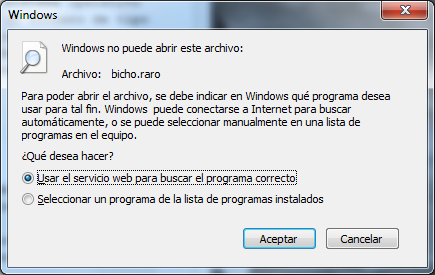
\includegraphics[height=6cm]{../fig/Tut00-AbriendoBichoRaro.png}
    \end{center}
Lo mejor, en la inmensa mayor parte de los casos, es seleccionar la opción {\tt Seleccionar un
programa de la lista de programas instalados} y pulsar en {\tt Aceptar}. En la ventana de diálogo
que aparece a continuación, puedes seleccionar el programa que deseas utilizar. Pero tienes que
prestar especial atención a los dos elementos que hemos indicado con flechas rojas en la figura.

    \begin{center}
    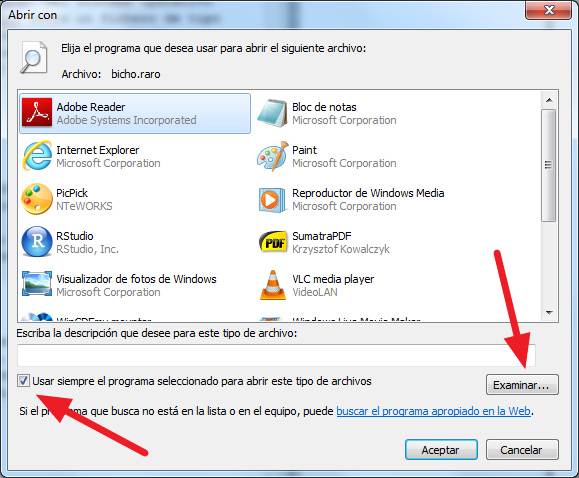
\includegraphics[height=6cm]{../fig/Tut00-SeleccionandoProgramaPredeterminado.png}
    \end{center}

La casilla {\tt Usar siempre el programa...} es especialmente importante, porque puede cambiar el
comportamiento de tu equipo, y tal vez no desees ese cambio. ¡Así que ve con cuidado! Si esa
casilla está marcada, y seleccionas el programa $A$ (el que quieras) para abrir un fichero de tipo
$B$, Windows modificará la lista a la que aludíamos antes, y escribirá en ella una línea
\begin{center}
{\em ``los ficheros de tipo $B$ se abren por defecto con el programa $A$''.}
\end{center}
Si no quieres que pase eso, debes desmarcar esta casilla. Por lo demás, si el programa que deseas
utilizar aparece en la ventana de la parte superior del cuadro de diálogo, basta con seleccionarlo
y pulsar {\tt Aceptar}. Cuando no es así, hay que usar el botón {\tt Examinar}, para localizar el
programa que queremos usar. Esta parte puede ser más o menos fácil, dependiendo del programa que se
trate, y de tu versión de Windows. Si tienes problemas para encontrar el programa, busca en
internet, o pide ayuda a alguien que sepa más que tú. En general ese consejo sirve no sólo para
este paso, sino para cualquiera de los siguientes. Siempre conviene tener un \ninja{ninja
informático} a mano.

\section{Navegador de internet.}
\label{tut00:sec:NavegadorInternet}

Para muchas de las tareas asociadas a este curso, la elección de uno u otro navegador de Internet
es irrelevante, siempre que se trate de versiones recientes. Pero para algunos temas concretos del curso es 
recomendable que utilices el navegador Firefox, que puedes descargar desde  este enlace:
\begin{center}
\link{http://www.mozilla.org/es-ES/firefox/new/}{http://www.mozilla.org/es-ES/firefox/new/}
\end{center}
Hay versiones disponibles para Windows, Mac y Linux. La razón por la que te recomendamos Firefox es
porque este navegador permite visualizar correctamente las fórmulas matemáticas, mientras que otros 
navegadores nos han causado más problemas al hacer esto
% \footnote{
% Desdichadamente, aunque hace más de una década que existe un lenguaje estándar para las fórmulas
% matemáticas en internet y el intercambio de contenido matemático entre programas, llamado MathML
% (\link{http://en.wikipedia.org/wiki/MathML}{http://en.wikipedia.org/wiki/MathML}) y creado por el
% consorcio W3C (\link{http://en.wikipedia.org/wiki/W3C}{http://en.wikipedia.org/wiki/W3C}, los
% navegadores han ignorado esta realidad durante mucho tiempo, complicando la creación de contenidos educativos
% accesibles para todos... La situación ha mejorado algo en las versiones más recientes.) } 
% Para que te hagas una idea del problema que esto puede representar, en esta
% figura aparece una misma fórmula de uno de nuestros cuestionarios,
%     \begin{center}
%     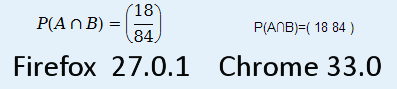
\includegraphics[height=2cm]{../fig/Tut00-SoporteMathMLNavegadores.png}
%     \end{center}
% Y como puedes ver, la fórmula que Chrome mostraba en esa versión tiene serios problemas de legibilidad, porque se
% llegan a perder incluso las barras de fracción. 
En cualquier caso, aparecen nuevas versiones de los navegadores muy a menudo. Y esas nuevas versiones pueden corregir algunos de esos problemas (desdichadamente, hemos tenido también experiencia con el proceso contrario, en el qu enua nueva versión estropeaba algo que ya estaba funcionando). Así que si quieres comprobar si tu navegador funciona correctamente puedes visitar esta pagina web: 
\begin{center}
\href{https://www.tuhh.de/MathJax/test/sample.html}{https://www.tuhh.de/MathJax/test/sample.html}
\end{center}
Espera unos segundos y asegúrate de que en tu navegador aparecen las fórmulas matemáticas como en esta figura:
    \begin{center}
    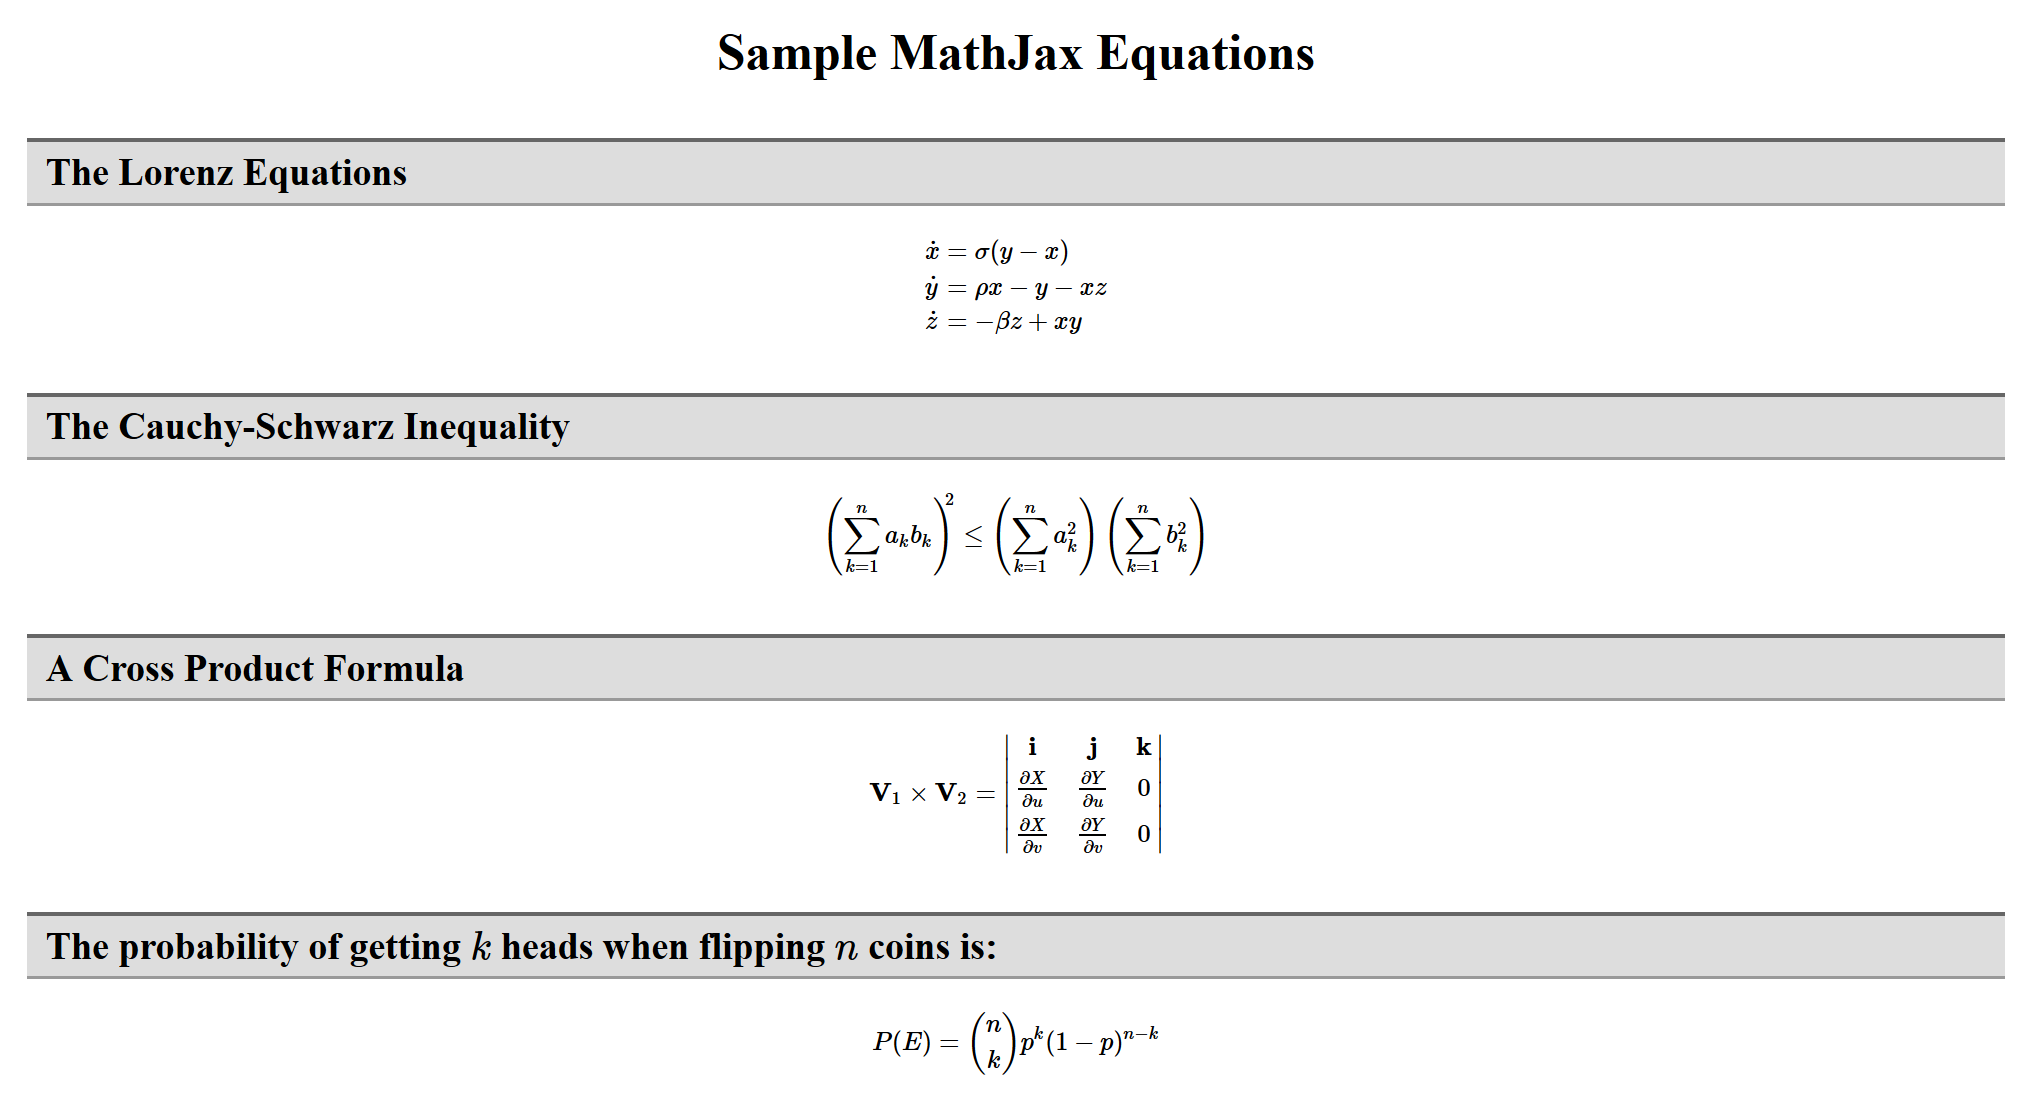
\includegraphics[width=12cm]{../fig/Tut00-18-MathJaxTest.png}
    \end{center}


\section{Instalación de la hoja de cálculo Calc.}
\label{tut00:sec:InstalacionCalc}

El siguiente paso es instalar, si no dispones ya de ella, la suite ofimática OpenOffice, que
incluye la hoja de cálculo Calc\footnote{Si tienes instalado o prefieres instalar
\link{http://es.libreoffice.org/}{LibreOffice}, no encontrarás apenas diferencia con OpenOffice, en
lo que se refiere a este curso.}, que vamos a utilizar, especialmente al principio del curso. Para
ello dirígete a
\begin{center}
    \link{http://www.openoffice.org/es/}{http://www.openoffice.org/es/}
\end{center}
y usa el enlace {\em Quiero descargar  OpenOffice}:
    \begin{center}
    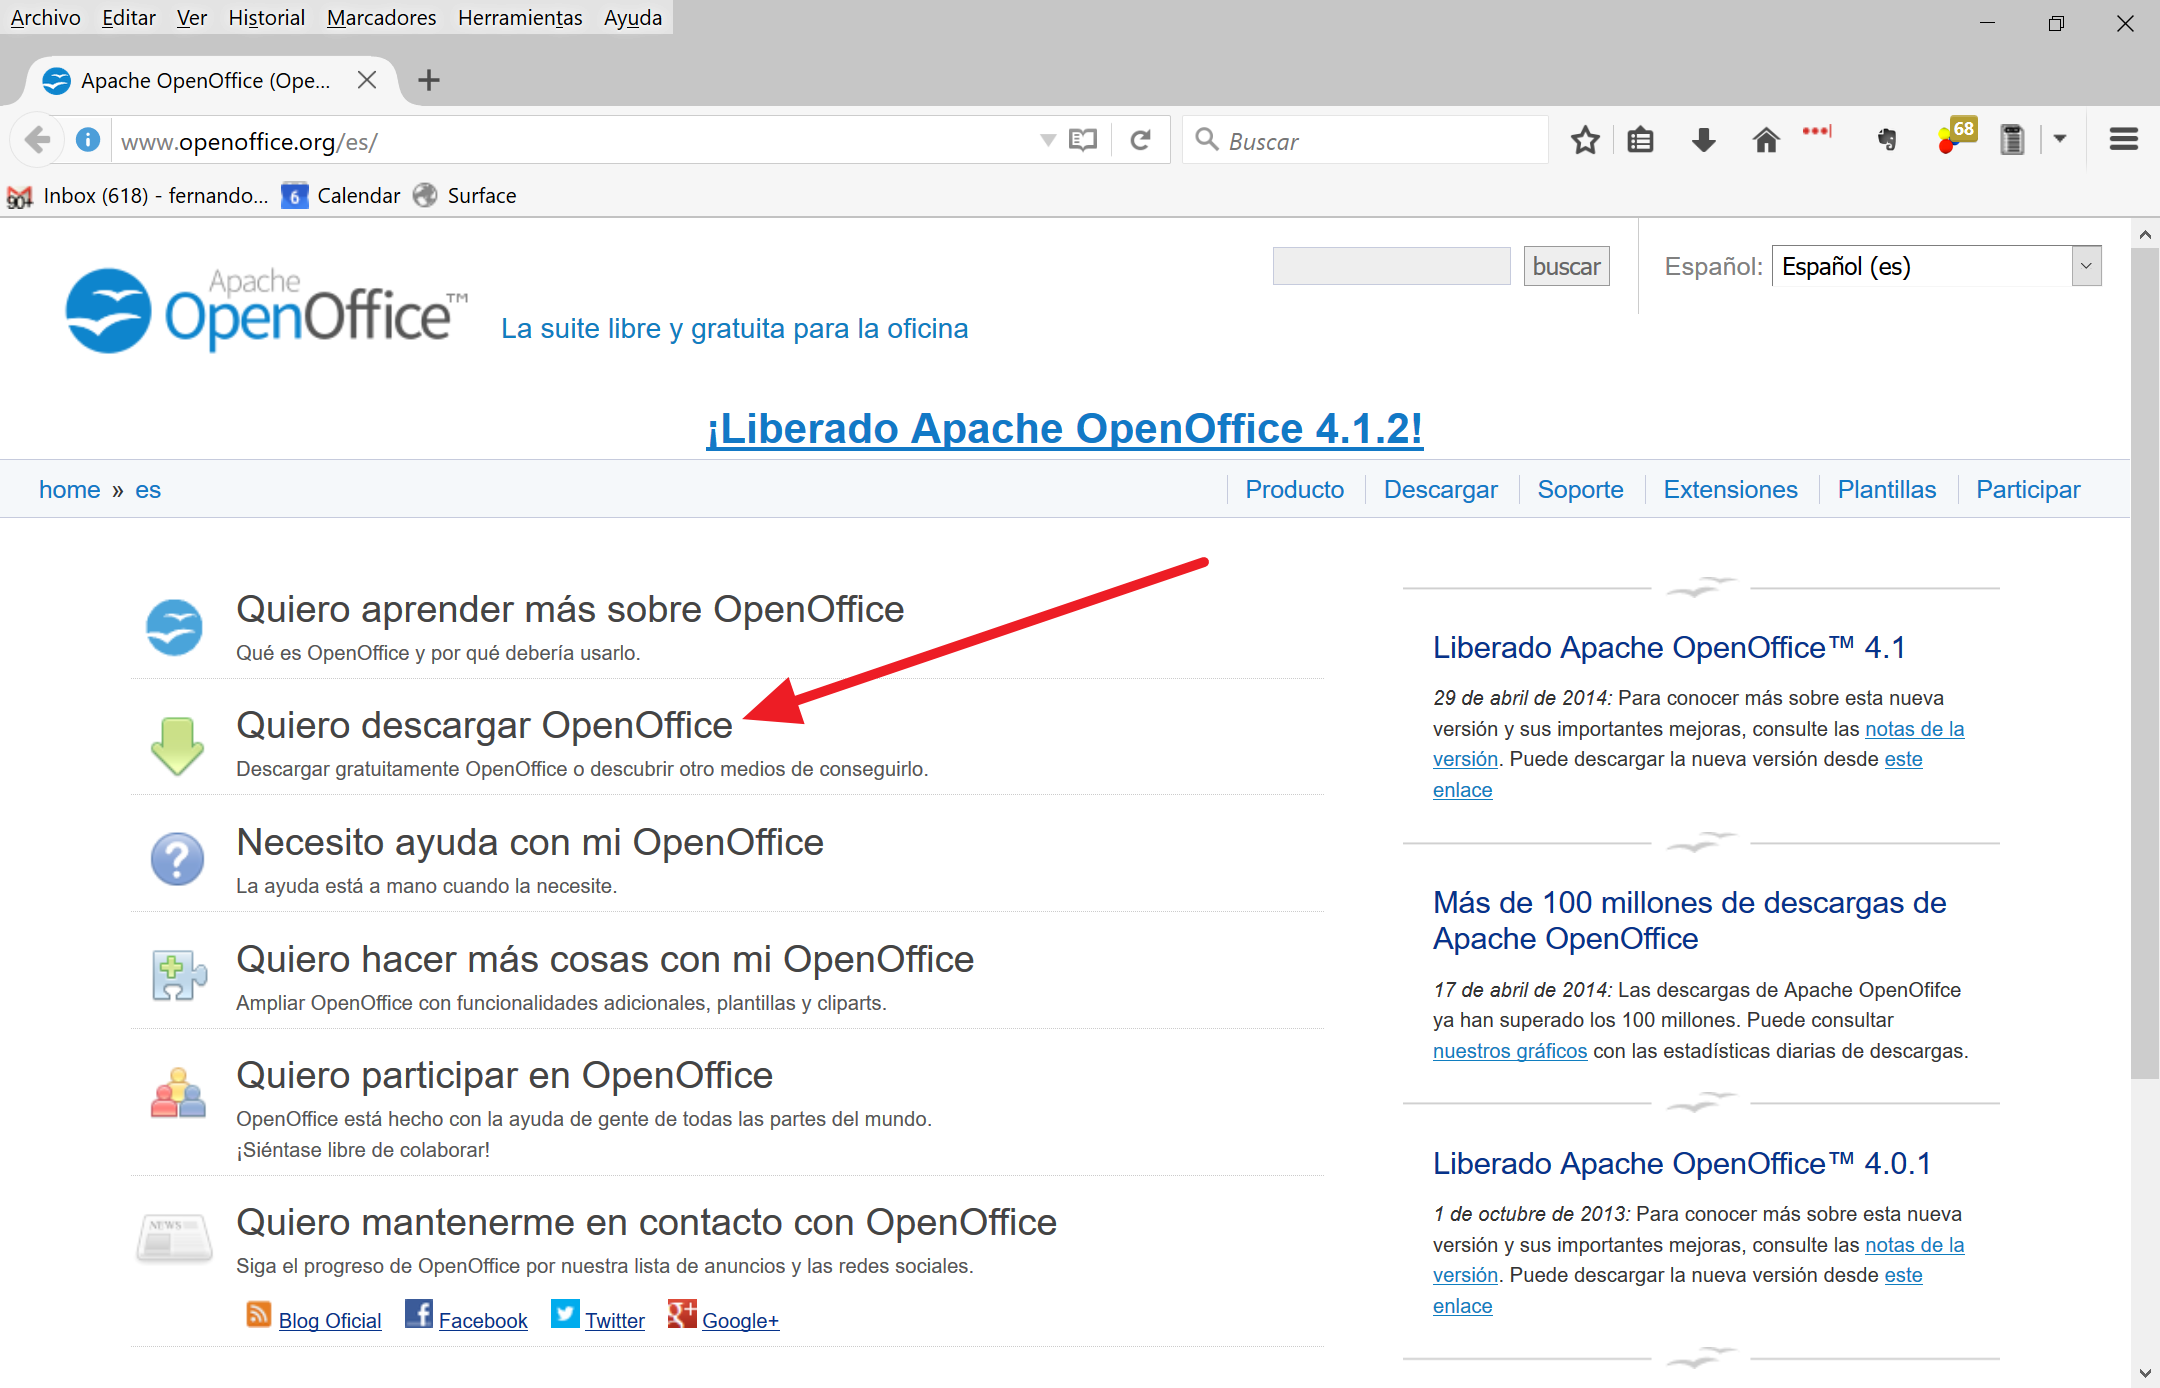
\includegraphics[height=9cm]{../fig/Tut00-WebOpenOffice-01-201605.png}
    \end{center}

Usando ese enlace, se abrirá la ventana que aparece en la siguiente figura, en la que debes hacer
clic en el enlace indicado por la flecha. ¡Asegurate de que seleccionas tu sistema operativo y el idoma español! El número de versión habrá cambiado, desde luego. En la
Figura aparece la versión {\tt 4.1.2}, pero en el momento en que tú la descargues, posiblemente habrá avanzado:
    \begin{center}
    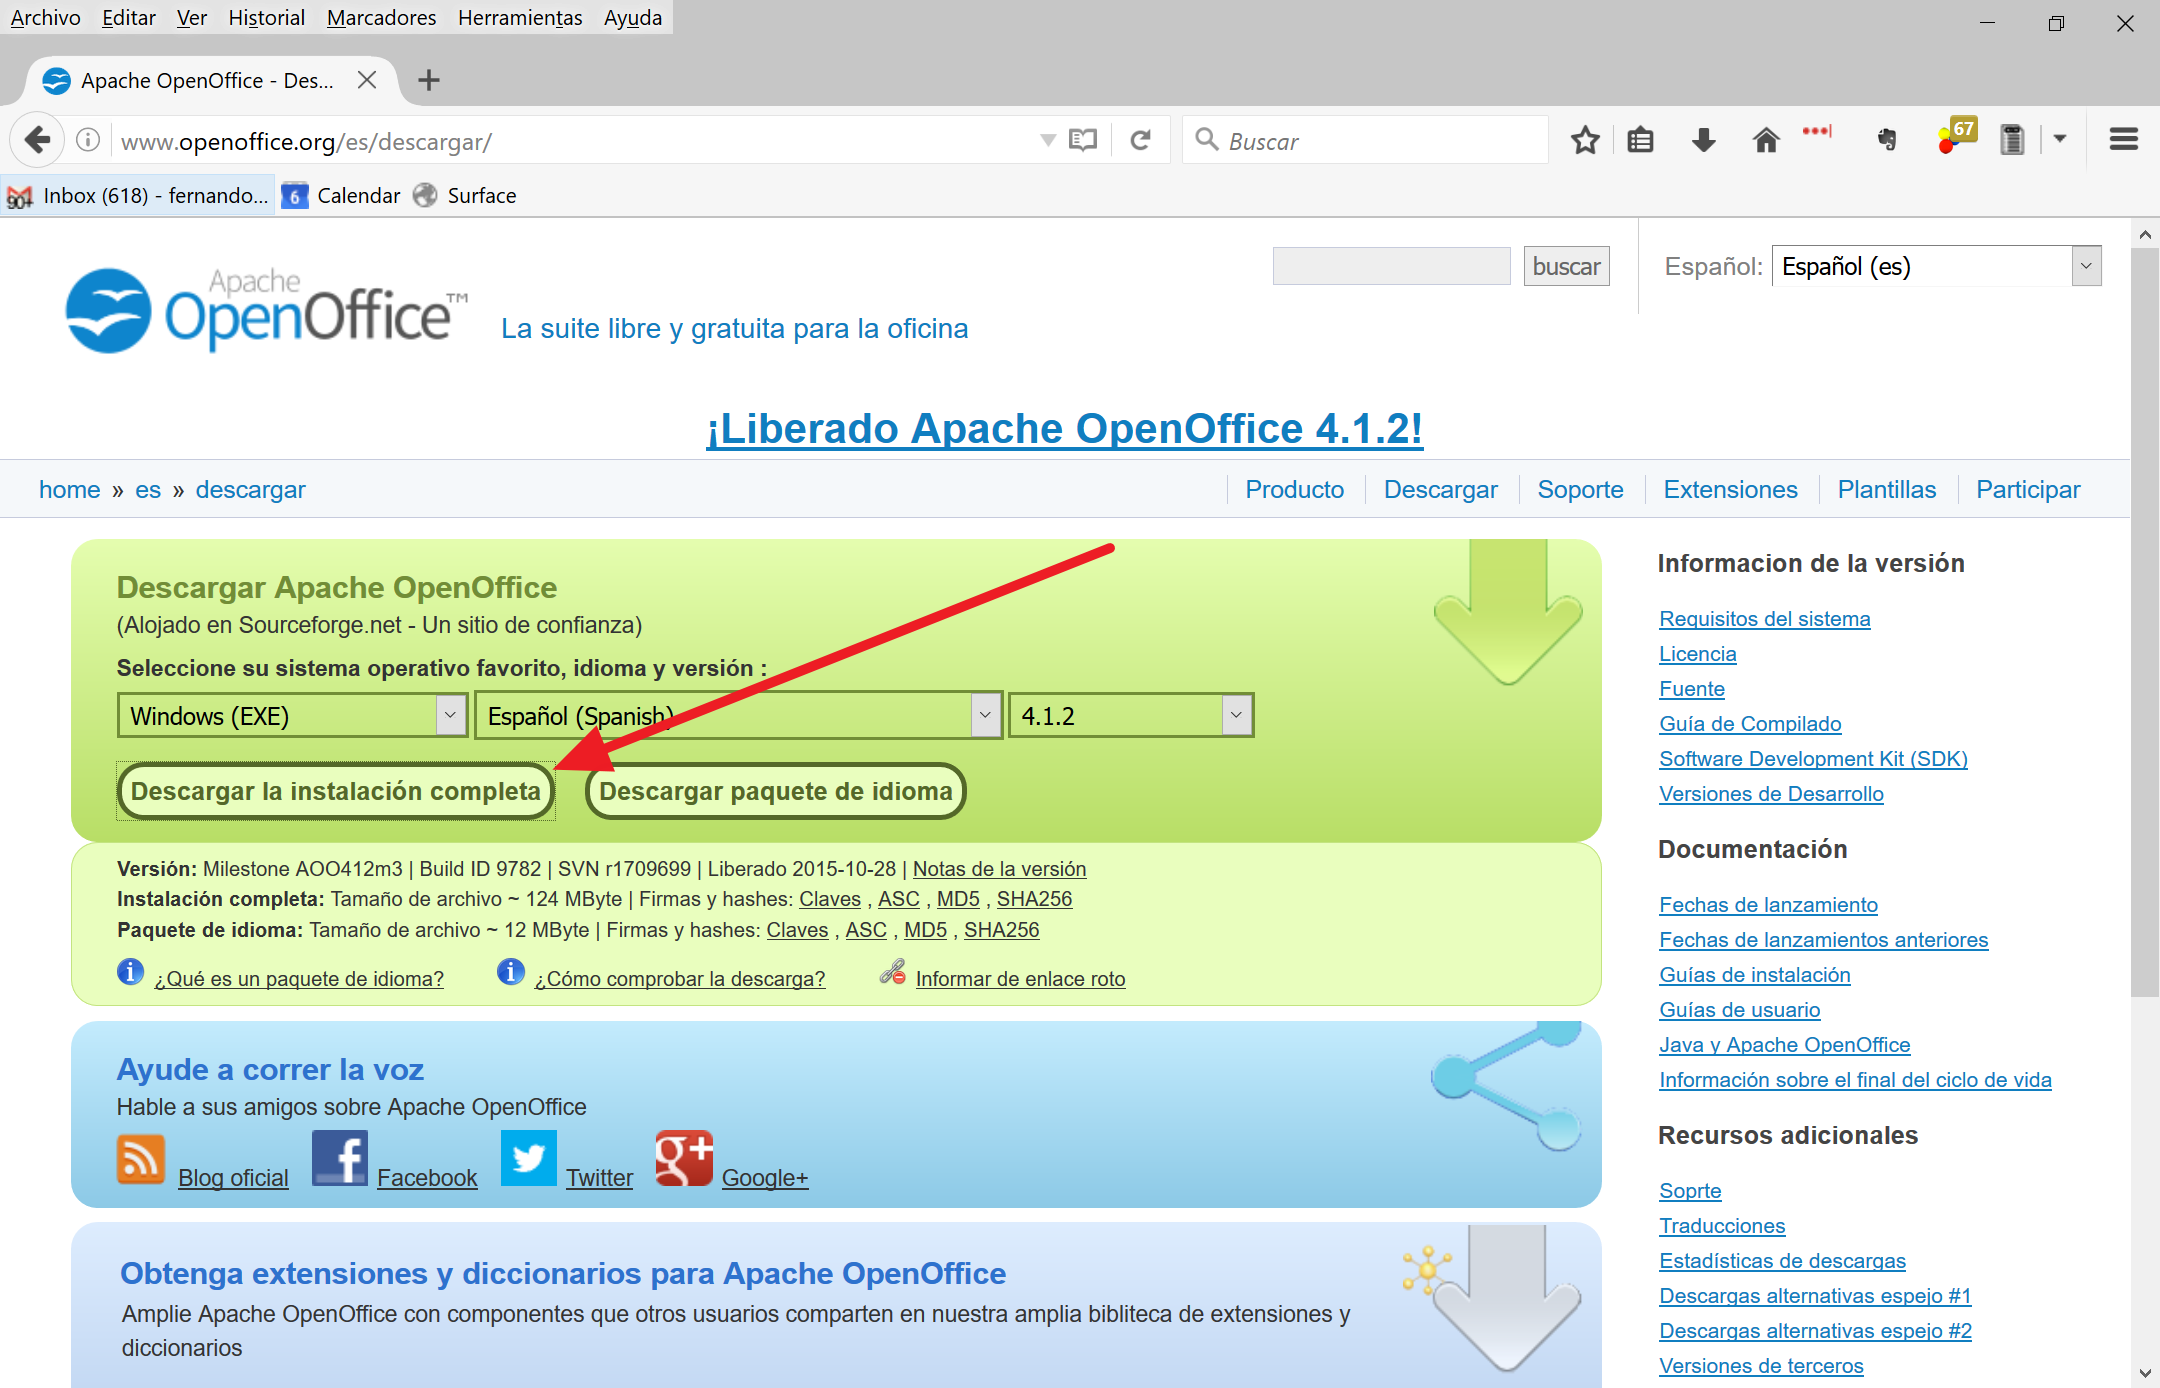
\includegraphics[height=9cm]{../fig/Tut00-WebOpenOffice-02-201605.png}
    \end{center}

Con eso llegamos a la página de descarga (alojada en el dominio {\tt sourceforge.net} a fecha de
hoy) y en pocos segundos, según la configuración del navegador, se descargará el archivo
automáticamente, o debe abrirse un cuadro de diálogo para guardar el fichero en alguna carpeta de
tu ordenador (por ejemplo, {\em Descargas} en máquinas Windows). Lo más importante en este paso es
que sepas en qué carpeta se guarda ese fichero, pero eso depende de tu configuración particular.

    \begin{center}
    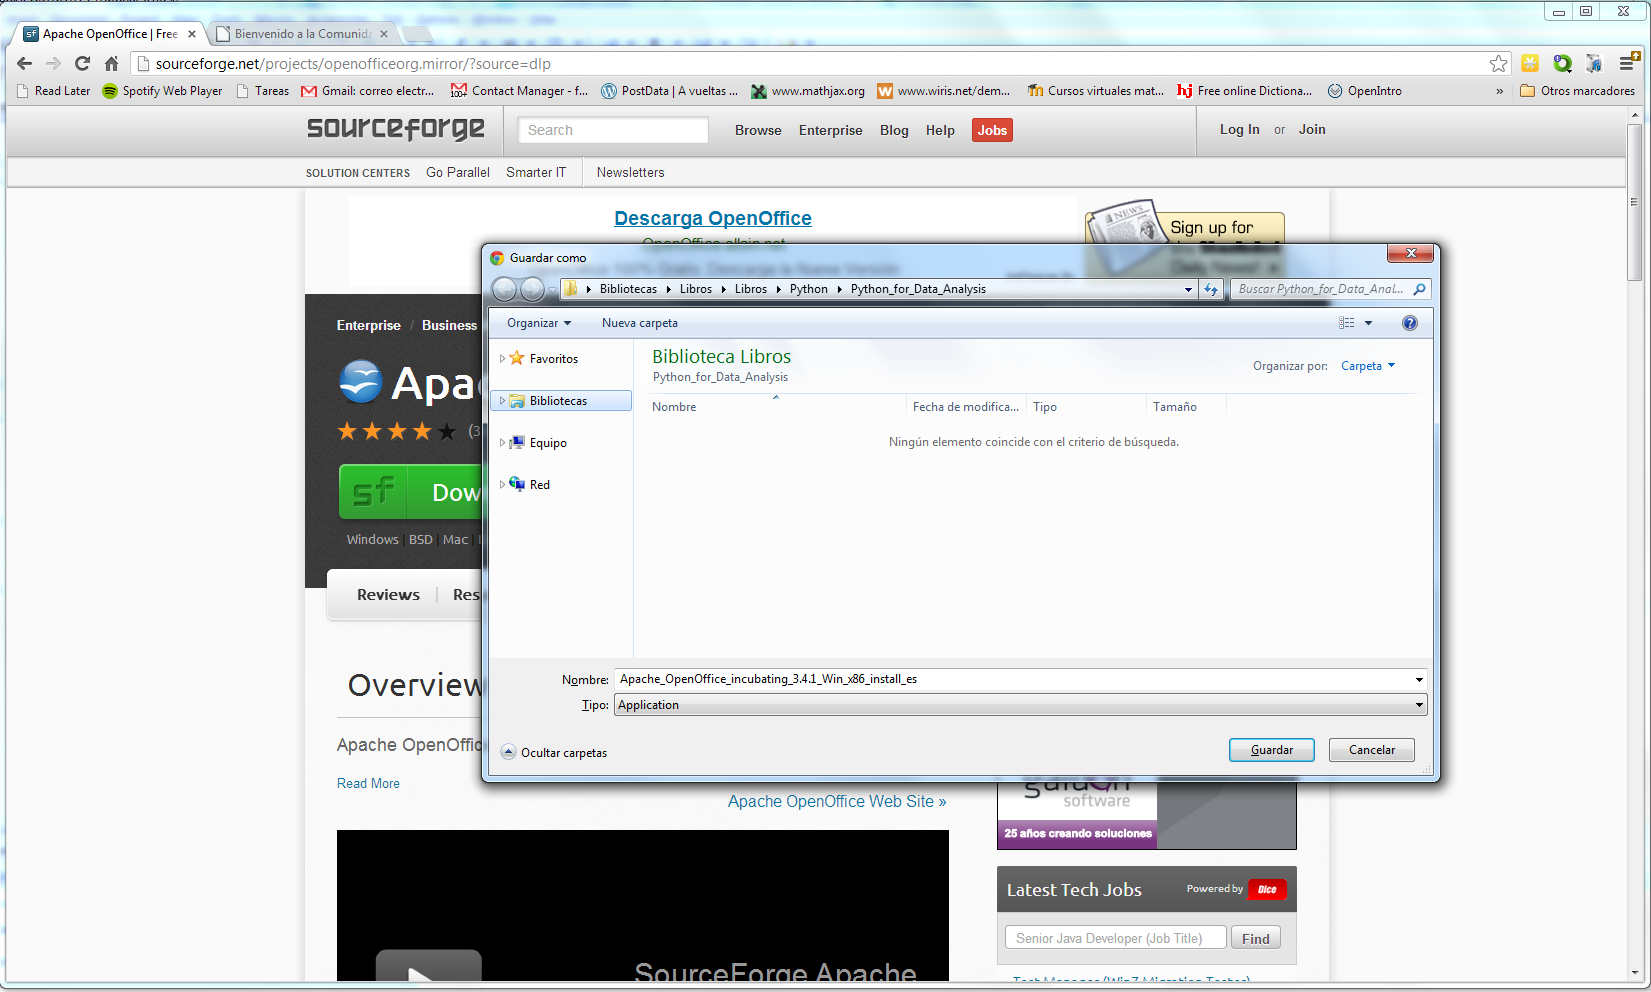
\includegraphics[height=7cm]{../fig/Tut00-WebOpenOffice-02.png}
    \end{center}

El fichero que has descargado se llamará (en Windows) algo parecido a:
\begin{center}
{\tt
Apache{\textunderscore}OpenOffice{\textunderscore}incubating{\textunderscore}4.1.2{\textunderscore}Winx{\textunderscore}86{\textunderscore}install{\textunderscore}es.exe}
\end{center}
(aunque puede que no veas la extensión {\tt .exe} en el Explorador de Windows). Ahora tienes que
abrir ese fichero, para instalar el programa (usa el botón derecho otra vez).  Para este paso, es
necesario disponer de permisos de administración en el ordenador (de nuevo, si te pierdes, busca al ninja...). En las últimas versiones de Windows, al hacer esto la pantalla se oscurece y aparece un
cuadro de diálogo que pregunta {\em ¿Desea permitir que este programa realice cambios...?}. Debes
pulsar en {\tt Sí} para continuar la instalación (insistimos, en las próximas figuras el número de
versión que aparecerá será otro, pero el proceso será esencialmente el mismo).
    \begin{center}
    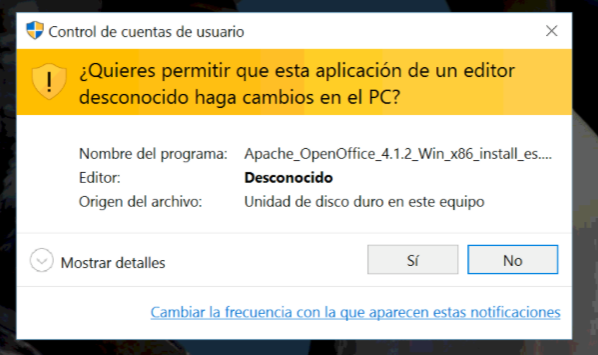
\includegraphics[height=4cm]{../fig/Tut00-OpenOffice-03-201605.png}
    \end{center}
Empieza la instalación:
    \begin{center}
    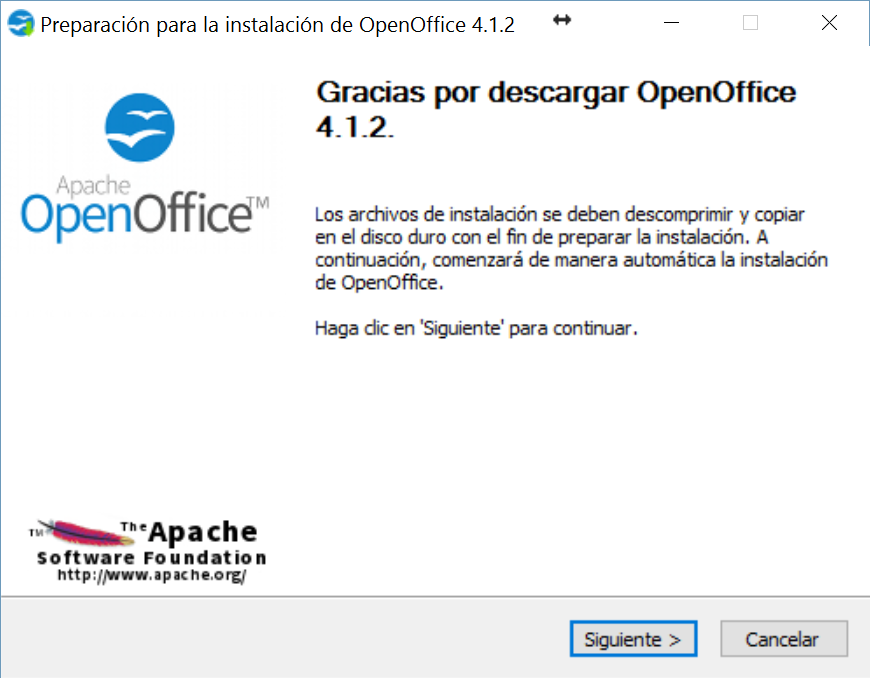
\includegraphics[width=7cm]{../fig/Tut00-OpenOffice-04-201605.png}
    \end{center}
La siguiente ventana te preguntará dónde quieres guardar una carpeta con los ficheros {\em
temporales} de instalación. Es importante, de nuevo, que recuerdes donde los guardas. Cuando
termine la instalación puedes borrar esa carpeta, sólo es necesaria durante la instalación.
    \begin{center}
    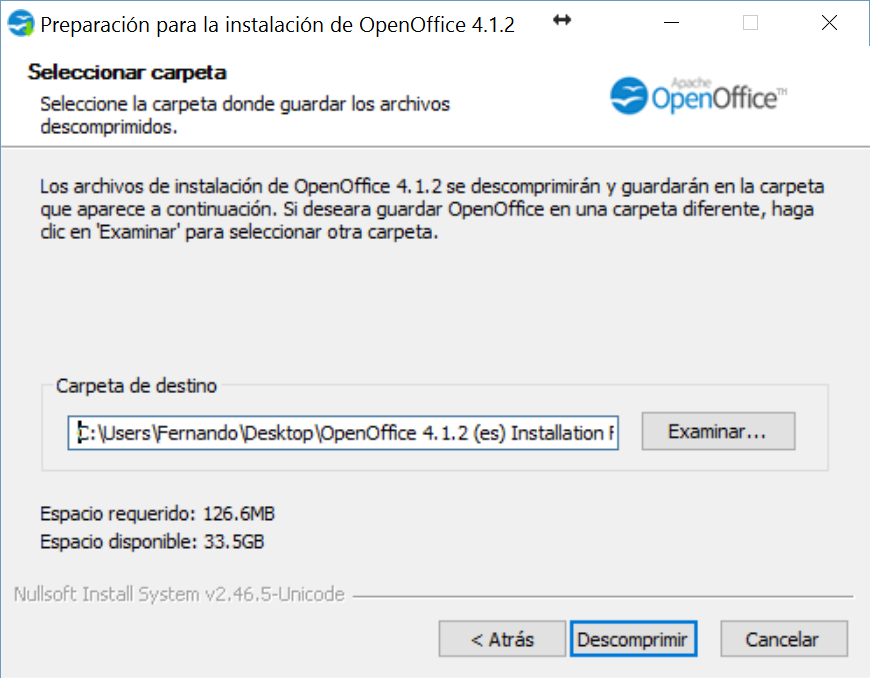
\includegraphics[height=5cm]{../fig/Tut00-OpenOffice-05-201605.png}
    \end{center}
A continuación el programa va pasando por pantallas similares a estas (son de una versión anterior), en las que puedes, 
sin riesgos, aceptar todas las opciones por defecto (en la segunda, si escribes tu nombre de usuario, se
incorporará a todos los documentos que crees con OpenOffice; puedes omitir esa información sin
problemas):
    \begin{center}
    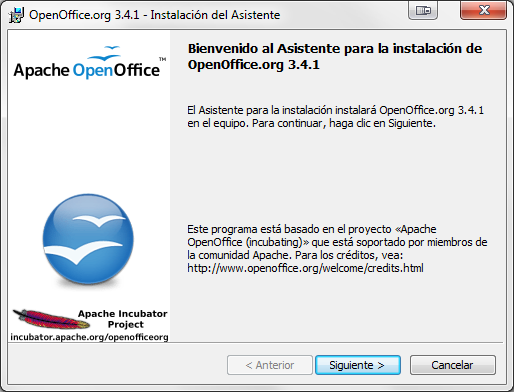
\includegraphics[width=7cm]{../fig/Tut00-WebOpenOffice-06.png}\hspace{1cm}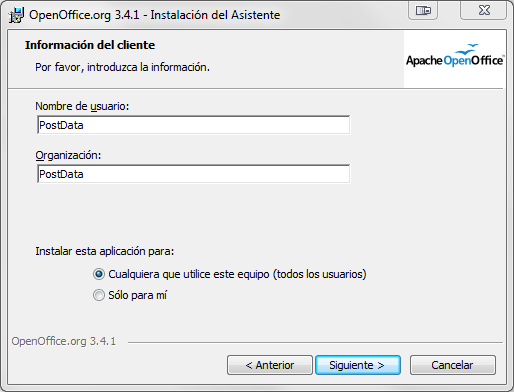
\includegraphics[width=7cm]{../fig/Tut00-WebOpenOffice-07.png}\\[5mm]
    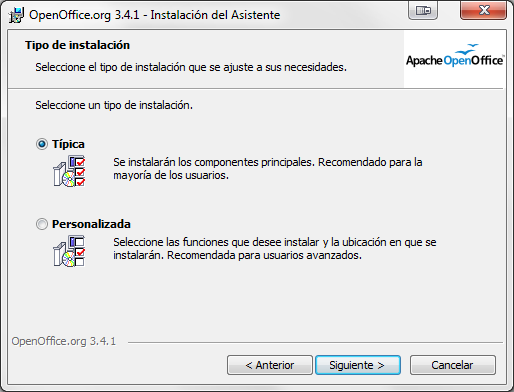
\includegraphics[width=7cm]{../fig/Tut00-WebOpenOffice-08.png}\hspace{1cm}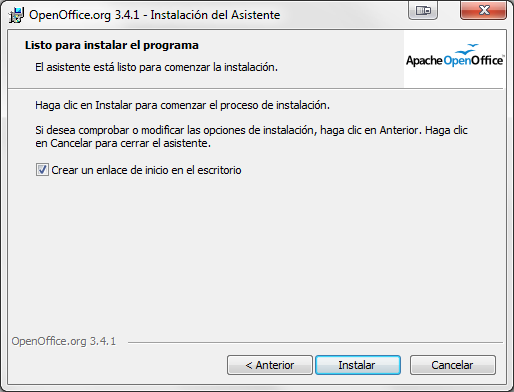
\includegraphics[width=7cm]{../fig/Tut00-WebOpenOffice-09.png}\\[5mm]
    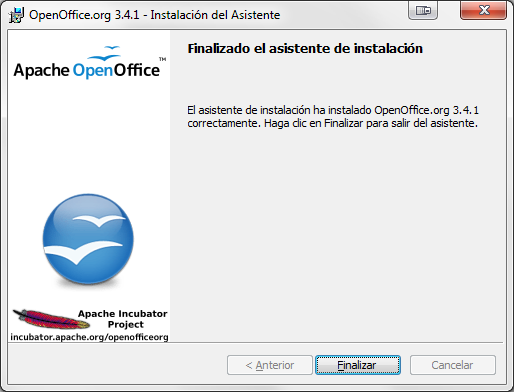
\includegraphics[width=7cm]{../fig/Tut00-WebOpenOffice-11.png}
    \end{center}
Al llegar a esta última ventana pulsa en {\tt Finalizar}, y la instalación habrá acabado. Ahora,
para comprobar que todo ha ido bien, deberías buscar en la lista de programas del menú Inicio (de
nuevo hablamos de Windows, aunque en otras plataformas es similar) el grupo de programas {\em
OpenOffice}, y abrir el que se llama {\em OpenOffice.org Calc}. Tras una ventana de presentación y
unos momentos, te encontrarás con esta pantalla (puedes verlo más o menos grande, según tu
resolución de pantalla):
    \begin{center}
    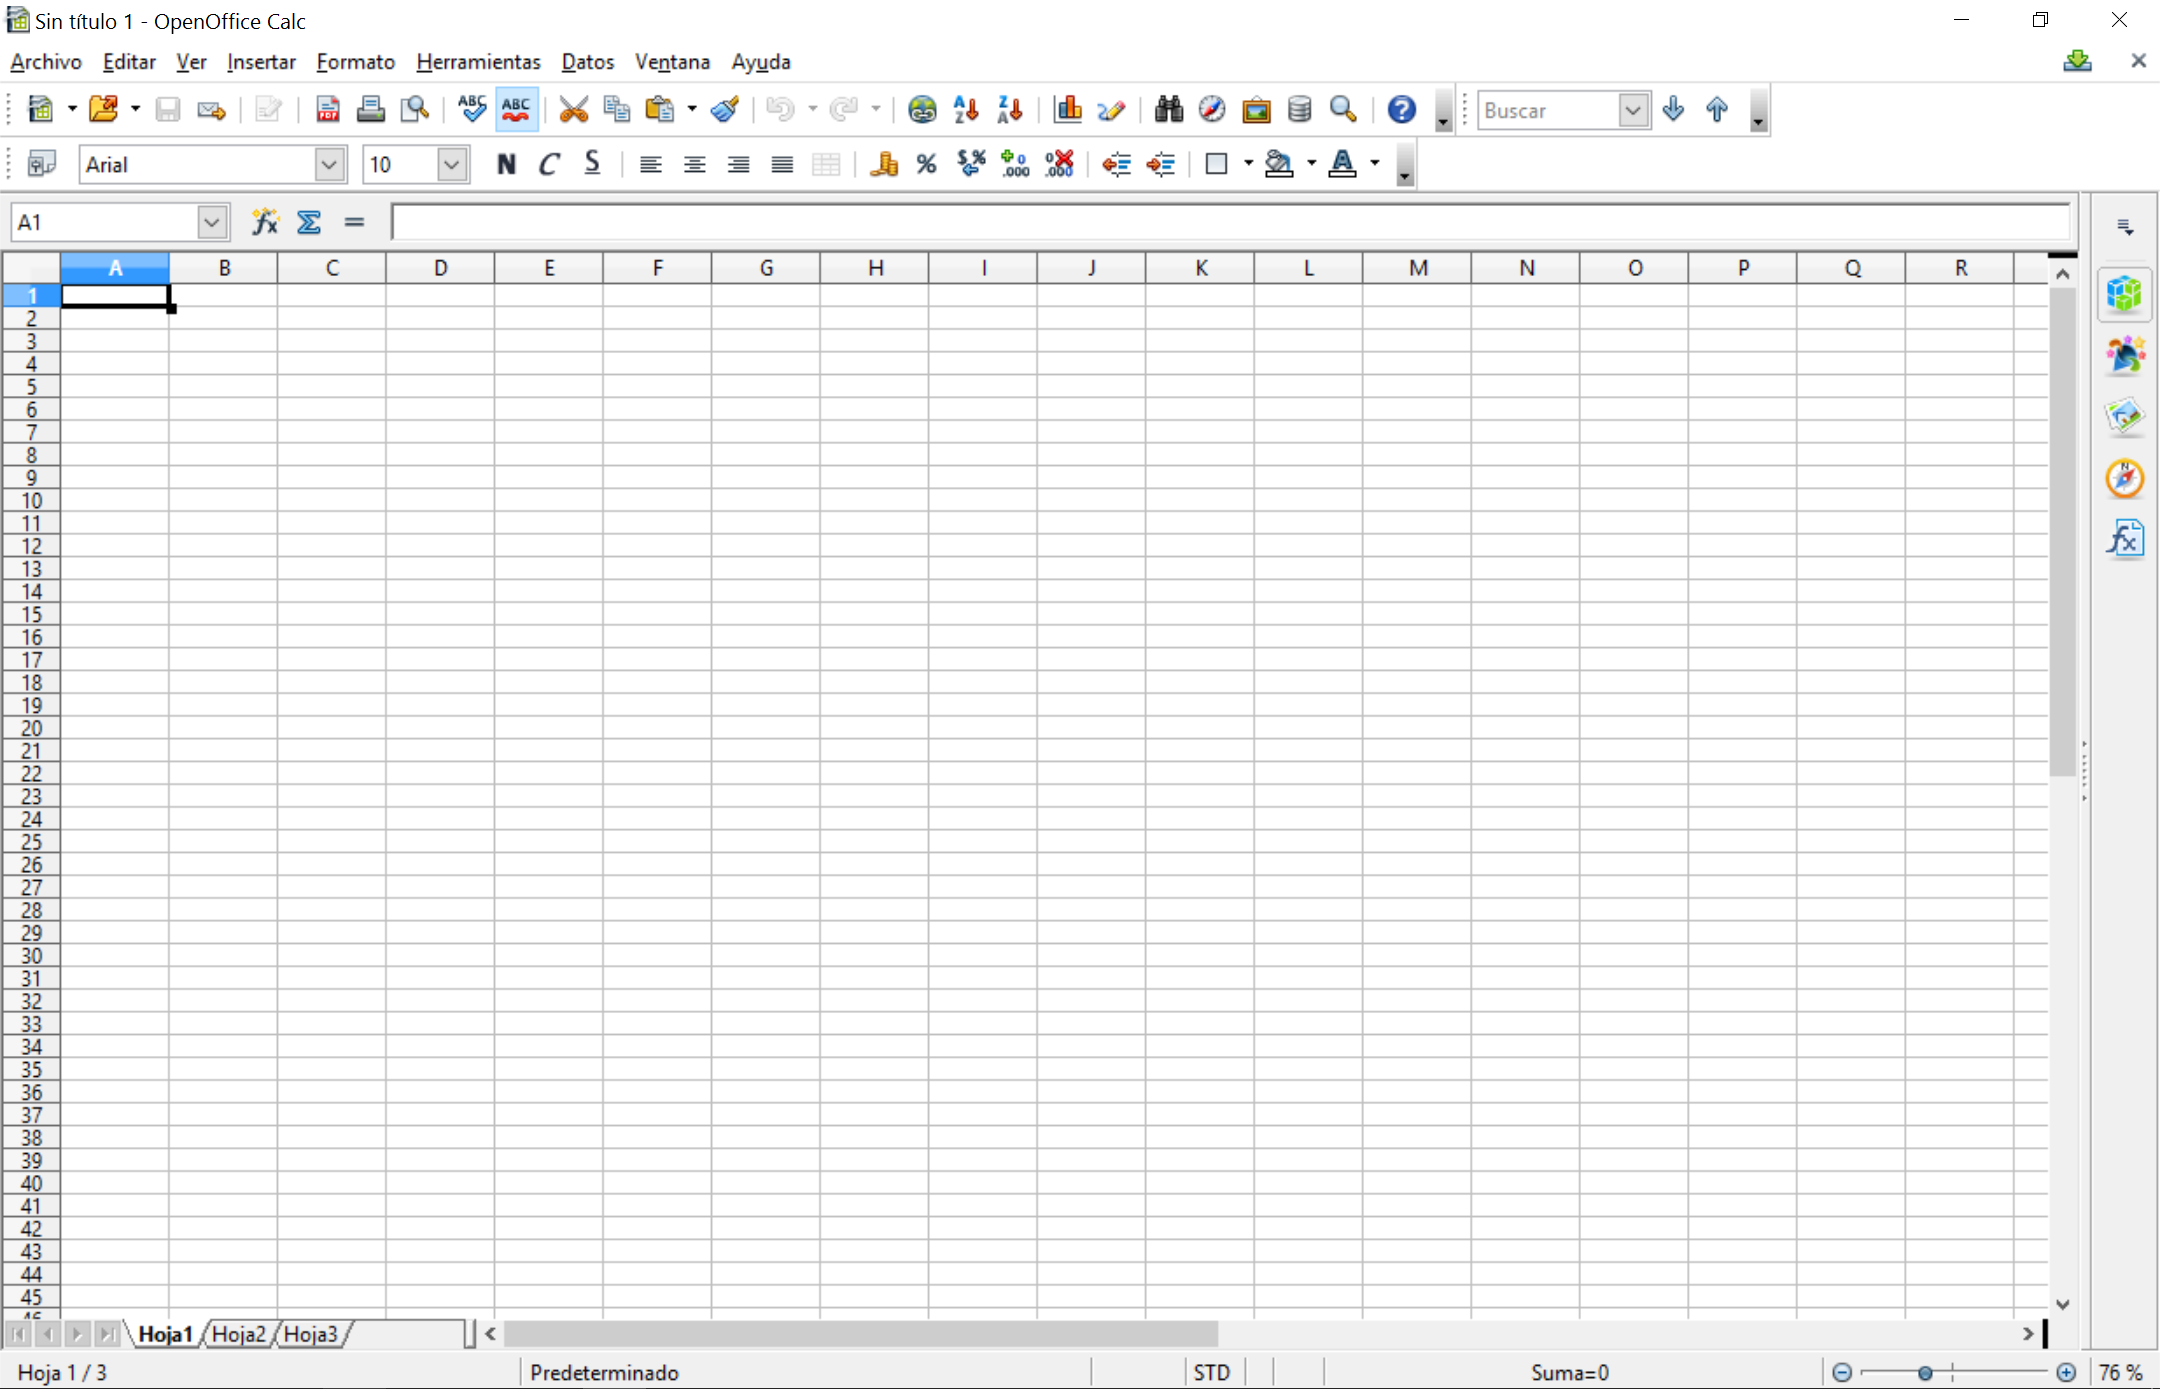
\includegraphics[height=10cm]{../fig/Tut00-OpenOffice-10-201605.png}
    \end{center}
que indica que todo ha ido bien. Ya estamos listos para pasar al segundo apartado de este tutorial.

\section{Editores de texto.}
\label{tut01:sec:EditoresTexto}

Nuestro objetivo, en esta sección, es localizar un {\em editor de texto}, como el {\em Bloc de
Notas} en Windows, y aprender a usarlo para abrir ficheros {\tt csv} (no te preocupes, enseguida
aprenderemos qué son estos ficheros). En segundo lugar, vamos a aprender a abrir ficheros de tipo
{\tt csv}  con Calc, eligiendo las opciones correctas en el menú de importación.

Empecemos por los editores de texto. En Windows, como ya hemos dicho, dispones del {\em Bloc de
Notas}. Si no lo localizas fácilmente, pulsa simultáneamente las teclas {\tt Windows} y {\tt R}, y
en el cuadro de diálogo que se abrirá escribe {\tt Notepad}. Tras pulsar en Aceptar se abrirá el
{\em Bloc de Notas} que, inicialmente tiene este aspecto:
\begin{center}
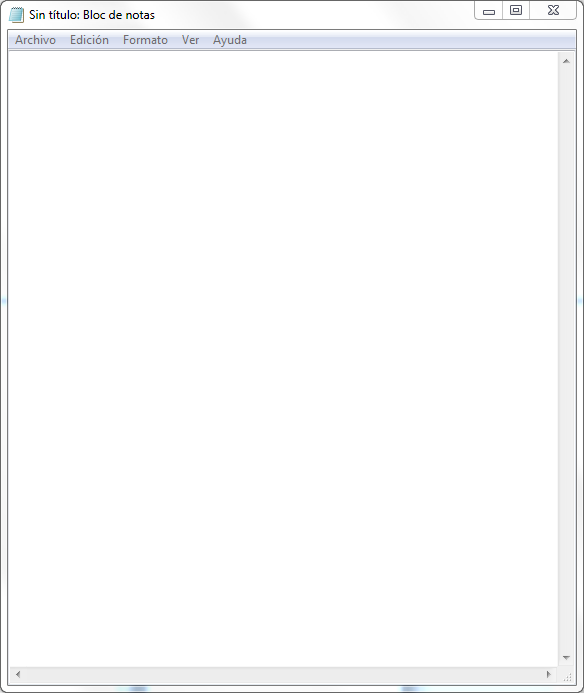
\includegraphics[width=10cm]{../fig/Tut00-BlocDeNotas.png}
\end{center}
En un Mac te recomendamos usar el programa gratuito {\tt
textwrangler}, que se descarga desde el enlace:
      \begin{center}
      \link{http://www.barebones.com/products/textwrangler/}{http://www.barebones.com/products/textwrangler/}
      \end{center}
TextEdit viene instalado en los Macs, pero no es exactamente un {\em editor de texto}, en el
sentido que aquí le damos a esa expresión (ver más abajo). Y si eres usuario de Linux, a buen
seguro ya conocerás algún editor de texto ({\tt kate, gedit, leafpad}, elige tu favorito).

Es importante que entiendas la diferencia entre los {\em procesadores de texto} y los {\em editores
de texto}. Un procesador de texto es un programa diseñado para la elaboración de textos, con un
enfoque esencialmente visual. El texto se puede formatear, cambiando el tipo y tamaño de letra,  la
tipografía (negrita, cursiva, subrayado), insertando imágenes, etc.  El ejemplo más conocido es el
programa {\em Word} de {\em Microsoft}. Al instalar {\em OpenOffice} en la sección anterior hemos
instalado otro procesador de texto, llamado {\em Writer}. En la siguiente figura puedes ver el
aspecto inicial de {\em Writer}, al abrir el programa, y compararlo con el del {\em Bloc de Notas},
que hemos visto antes.
    \begin{center}
    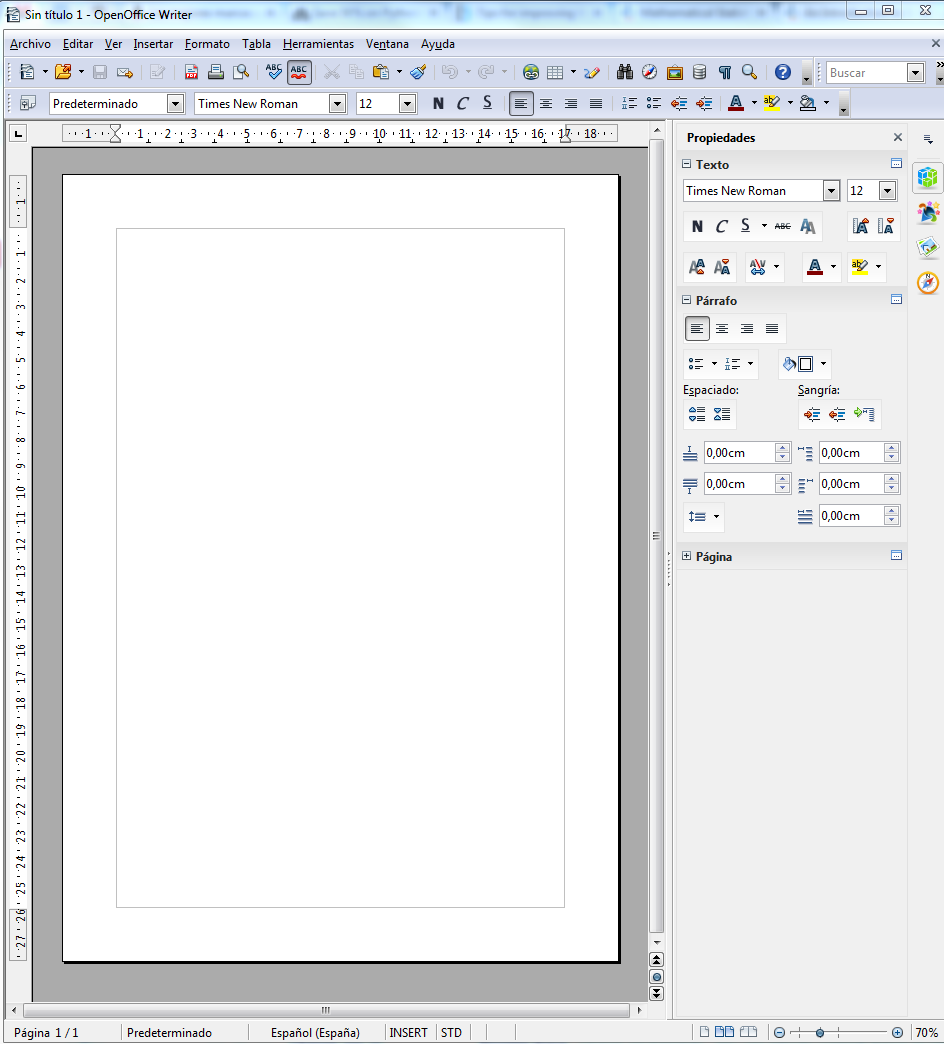
\includegraphics[height=11cm]{../fig/Tut00-ProcesadorVsEditor.png}
    \end{center}
El contraste entre el procesador de texto, lleno de herramientas de formato, y el aspecto casi
vacío del editor de texto, debería ser evidente. Naturalmente, hay editores de texto más
sofisticados que el {\em Bloc de Notas} (por ejemplo, en Windows,
\link{http://notepad-plus-plus.org/}{Notepad++}), pero lo más importante es que comprendas que los
procesadores de texto {\em no son adecuados} para el trabajo con los ficheros que vamos a usar en
este curso, que son ficheros de {\em texto plano}. Los ficheros de texto plano más conocidos son
los de extensión {\tt txt}, pero hay muchos otros tipos. Por ejemplo, los ficheros de datos de tipo
{\tt csv} que vamos a ver a continuación. Pero también son ficheros de texto plano los ficheros de
{\sf código fuente} (en inglés, {\em source code}) de la mayoría de lenguajes de programación.
Nosotros, en este curso, vamos a usar ficheros de código para el programa R, que serán ficheros de
texto plano, con la extensión {\tt .R}.

\section{Ficheros {\tt csv} con Calc.}
\label{tut00:sec:FicherosCsvConCalc}

Un fichero {\tt csv} es un fichero de texto plano que contiene una tabla de datos. El nombre
proviene del inglés, {\em comma separated values} (valores separados por comas, aunque ya veremos
que no hay que tomarse el nombre al pie de la letra).  Para empezar, vamos a trabajar con el
fichero (que también usaremos en el Tutorial-01)
\begin{center}
\fichero{../datos/Tut01-PracticaConCalc.csv}{Tut01-PracticaConCalc.csv}.
\end{center}
Te aconsejamos que {\em guardes} el fichero, en lugar de {\em abrirlo} directamente (y no olvides
dónde lo has guardado; el {\em Escritorio} puede servir, para empezar). Recuerda lo que hemos
visto en la Sección \ref{tut00:sec:InstalacionGeoGebra}: el fichero de datos va {\em adjunto} a
este documento pdf y, para guardar los datos en tu ordenador, debes hacer clic (aquí mismo, en el
documento pdf) sobre el nombre del fichero. ¿Clic derecho o izquierdo? Depende del lector de pdfs
que estés usando. ¡Recuerda que en muchos casos es mejor usar primero el botón derecho del ratón!
Si no sabes bien lo que haces, este es otro paso en el que es posible que te pierdas. Si eso
sucede, será un buen momento para acudir a \ninja{nuestro amigo.} Y, en cualquier caso, recuerda
que también puedes descargar todos los ficheros adjuntos del curso (teoría o tutoriales) desde la
página web del curso, a la que se llega mediante este enlace:
\begin{center}
\link{http://www.postdata-statistics.com/}{http://www.postdata-statistics.com/}.
\end{center}

Los ficheros {\tt csv} se usan para guardar datos de una forma sencilla, en ficheros de texto,
facilitando así el intercambio de datos entre programas. El fichero  {\tt
Tut01-PracticaConCalc.csv} es un ejemplo típico: contiene una tabla de datos con tres columnas, y
1300 filas. Es una buena idea que empieces por abrirlo con un editor de texto (el {\em Bloc de
Notas} en Windows, o similar) para hacerte una idea del aspecto que tienen los datos, pero no hagas
ningún cambio en el fichero. En la siguiente figura puedes ver el aspecto de ese fichero cuando se
abre con el  {\em Bloc de Notas} de Windows.
    \begin{center}
    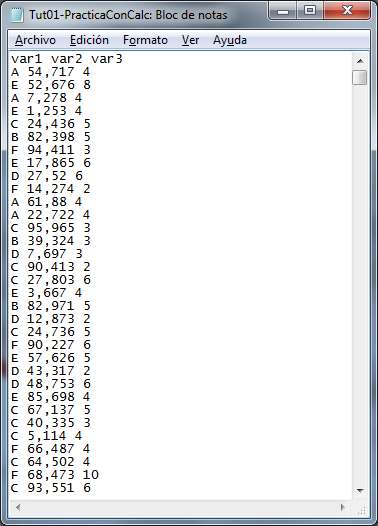
\includegraphics[height=9cm]{../fig/Tut00-AbriendoFicheroCsvBlocDeNotas.png}
    \end{center}
En este fichero en particular, hay guardada una tabla de tres columnas. Cada fila de la tabla se
corresponde con una línea del fichero, y los elementos de las distintas columnas están separados
por espacios. La primera línea es especial, porque contiene los nombres de las variables que
corresponden a cada columna, y que son {\tt var1, var2} y {\tt var3}. Usando el editor de texto
podemos ver los datos que contiene el fichero, e incluso hacer algunas modificaciones muy
interesantes. Por ejemplo, podemos reemplazar todas las comas por puntos o viceversa. Pero el
procesador de texto no sirve para analizar los datos desde el punto de vista estadístico. Para eso
necesitamos herramientas más especializadas, como la hoja de cálculo, que vamos a ver a
continuación; o programas específicos de Estadística, como R, que veremos en próximos tutoriales.

Es una excelente idea echarle un vistazo al fichero csv con un editor de texto antes de lanzarnos a
hacer otras operaciones. Considéralo el primer paso de la descripción estadística de los datos,
llamada también {\em Análisis Exploratorio de Datos}.

\subsection{Abriendo el fichero con Calc.}

Si no lo has hecho, cierra el editor de texto en el que hemos abierto el fichero {\tt csv}. Para
seguir avanzado, vamos a abrirlo con la hoja de cálculo Calc. Una vez iniciado Calc, usa el menú
{\tt Archivo $\to$ Abrir} y navega hasta la carpeta en la que has guardado el fichero {\tt
Tut01-PracticaConCalc.csv}. Cuando lo selecciones para abrir se debería abrir un cuadro de diálogo
como el de la siguiente figura, que vamos a analizar:
        \begin{center}
        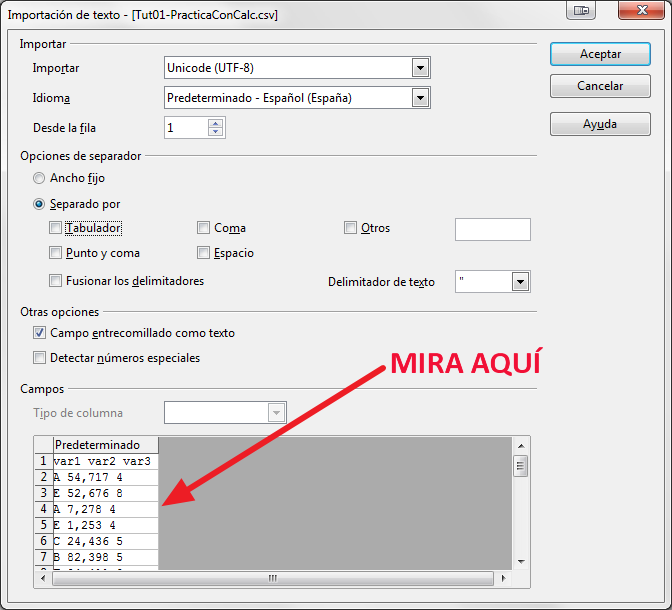
\includegraphics[height=8cm]{../fig/Tut00-Calc-csv-01.png}
        \end{center}
Hemos indicado con una flecha roja la primera zona en la que debes fijarte. Calc te muestra una
vista previa de su interpretación del fichero de datos. En el caso que se muestra en la figura, esa
interpretación no coincide con lo que nosotros queremos obtener. Ten en cuenta que en tu ordenador
las cosas pueden ser distintas, porque la interpretación de Calc depende de las opciones que se
hayan seleccionado en la zona del cuadro de diálogo que hemos destacado en esta figura:
        \begin{center}
        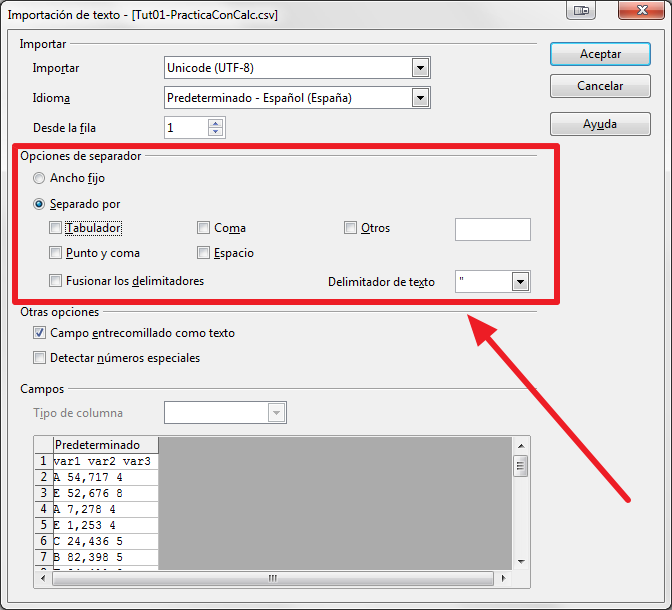
\includegraphics[height=9cm]{../fig/Tut00-Calc-csv-02.png}
        \end{center}
Aunque los ficheros {\tt csv} deban su nombre a las comas, en realidad, se pueden usar (y se usan)
distintos símbolos como {\sf separadores} entre las distintas columnas de la tabla de datos que
contiene el fichero. En los países que, como España, usan la coma como separador del punto decimal,
es habitual usar un espacio, o un punto y coma, o un tabulador para separar entre sí las columnas.
Esa parte del cuadro de diálogo nos deja seleccionar cuál (o cuáles, a veces son varios) de los
símbolos posibles se deben interpretar como símbolos de separación entre columnas. En este ejemplo,
las columnas están separadas por un espacio. Así que marcamos la casilla de la opción {\tt
Espacio}, nos aseguramos de que no haya seleccionada ninguna otra opción, y,  como en esta figura,
vemos en la vista previa que ahora Calc está interpretando los datos como queremos que lo haga.
        \begin{center}
        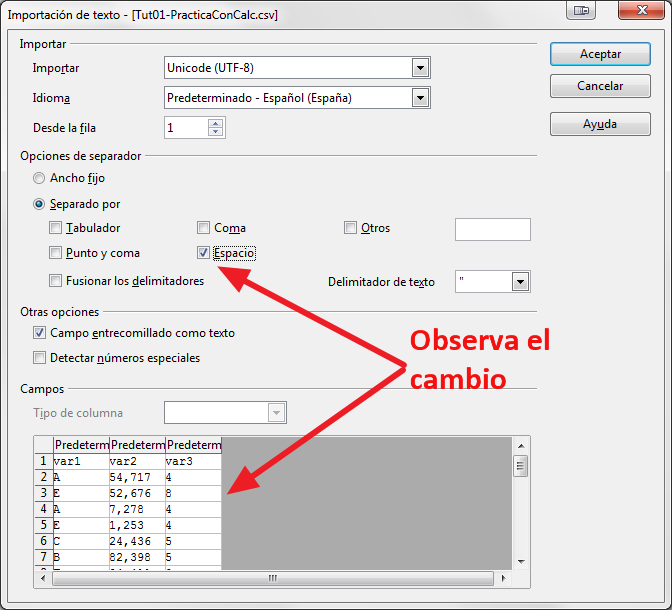
\includegraphics[height=9cm]{../fig/Tut00-Calc-csv-03.png}
        \end{center}
        Ahora podemos pulsar en {\tt Aceptar}, y veremos como Calc nos muestra los datos, colocando correctamente las columnas de nuestra tabla de datos.
        \begin{center}
        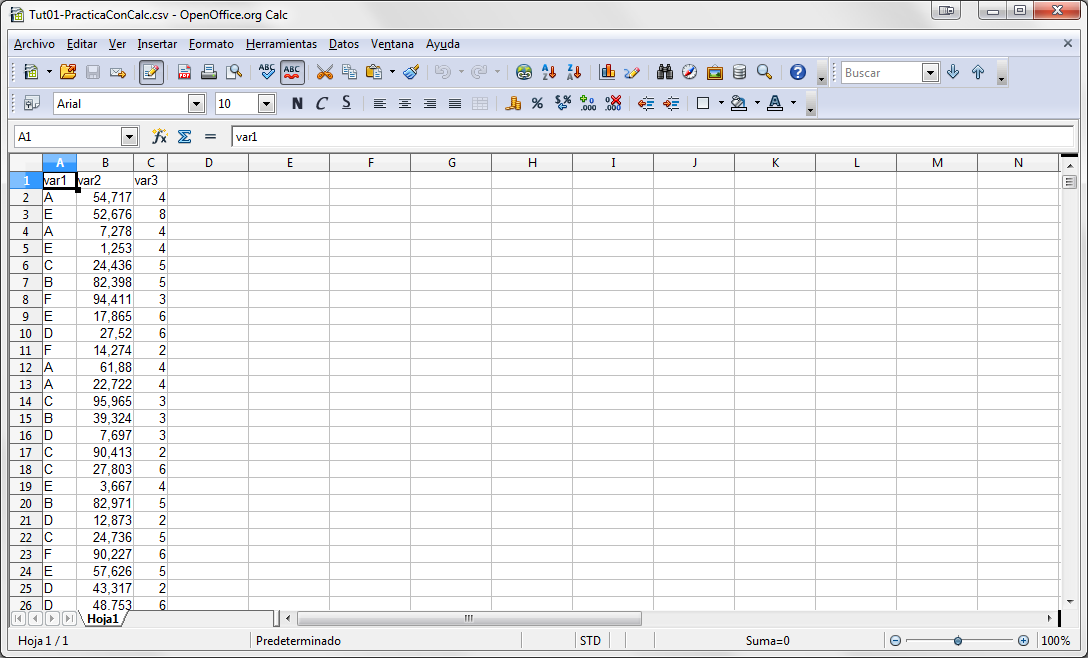
\includegraphics[height=9cm]{../fig/Tut00-Calc-csv-04.png}
        \end{center}
En el próximo tutorial empezaremos a trabajar con estos datos. Pero, antes de abandonar esta
sección, queremos inaugurar una costumbre que nos va a acompañar en todos los tutoriales del curso.
De vez en cuando te propondremos un ejercicio, para que puedas practicar lo que acabamos de
aprender.

\newcounter{EjercicioI}
\stepcounter{EjercicioI}
\paragraph{Ejercicio \theEjercicioI:}\quad\\
\begin{enumerate}
  \item Trata de repetir los pasos anteriores, para abrir en Calc el fichero adjunto:
        \begin{center}
        \fichero{../datos/Tut00-Ejercicio01a.csv}{Tut00-Ejercicio01a.csv}
        \end{center}
        Es recomendable empezar explorando el fichero con un editor de texto.
  \item ¿De qué tipo crees que son las variables de cada una de las columnas?
  \item {\em El juego de las diferencias:} Trata de repetir los pasos anteriores para abrir en
      Calc el fichero adjunto:
        \begin{center}
        \fichero{../datos/Tut00-Ejercicio01b.csv}{Tut00-Ejercicio01b.csv}
        \end{center}
        que contiene exactamente los mismos datos, pero con algunas modificaciones en la forma en
        la que se han codificado en el fichero. ¿Qué diferencias son esas?
\end{enumerate}
\qed


\subsection{Esquila de datos. Modificando ficheros csv con un editor de texto.}

El fichero {\tt Tut00-Ejercicio01b.csv} del Ejercicio {\theEjercicioI} contiene una columna (la
segunda, de nombre {\tt medidas}), en la que se ha usado el punto, en lugar de la coma, como
separador decimal. Eso puede suponer un problema para nosotros, porque algunos programas de
ordenador usan la coma como separador decimal (por ejemplo, Calc en la versión en español),
mientras que otros usan el punto (por ejemplo, R). Es frecuente, por tanto, encontrarse en la
situación de tener que modificar un fichero de datos para cambiar puntos por comas, o viceversa.
Esta es una operación típica (y sencilla) de lo que vamos a denominar {\sf Esquila de Datos}. Es
nuestra traducción del inglés {\em Data Wrangling}. Otra gente diría que están domando o
domesticando datos, pero nosotros somos más de oveja, qué se le va a hacer.

Lo que tenemos que hacer, entonces, es cambiar los puntos por comas. Esta tarea, que en general
consiste en reemplazar una cadena de texto por otra, la podemos acometer con un editor de texto
sencillo como el {\em Bloc de Notas} de Windows. Vamos a dar los detalles para el {\em Bloc de
Notas}, pero no deberías tener problemas en reproducirlos  usando sus análogos en otros sistemas.

Al abrir el fichero {\tt Tut00-Ejercicio01b.csv} con el {\em Bloc de Notas} veremos esto (sólo una
parte del fichero resulta visible, dependiendo del tamaño de la ventana del editor en tu pantalla):
        \begin{center}
        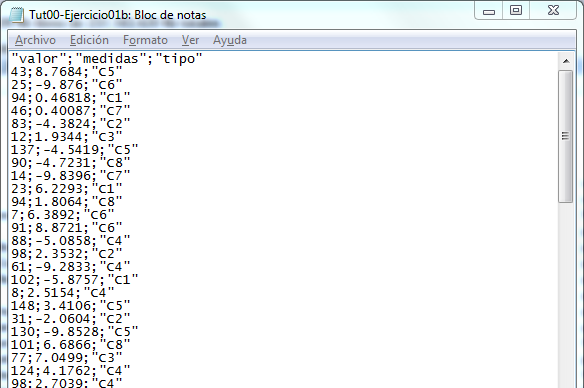
\includegraphics[width=11cm]{../fig/Tut00-EjercicioI-a.png}
        \end{center}
En el menú {\tt Edición}, seleccionamos {\tt Reemplazar...} (o pulsa {\tt Ctrl+ R}):
        \begin{center}
        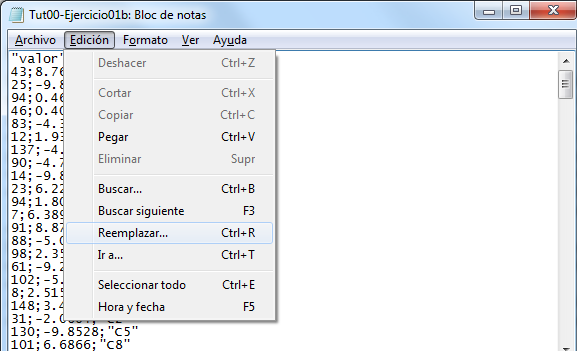
\includegraphics[width=11cm]{../fig/Tut00-EjercicioI-b.png}
        \end{center}
En el cuadro de diálogo que aparece escribe un punto en {\tt Buscar} y una coma en {\tt Reemplazar
por}, como indica la figura:
        \begin{center}
        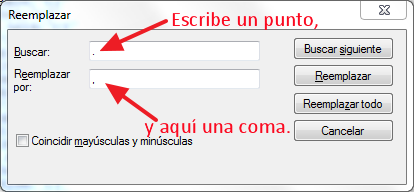
\includegraphics[width=9cm]{../fig/Tut00-EjercicioI-c.png}
        \end{center}
Luego pulsa {\tt Reemplazar todo}. Aunque el cuadro de diálogo no se cierra, los cambios ya se han
hecho. Puedes cerrar ese cuadro de diálogo para verlo:
        \begin{center}
        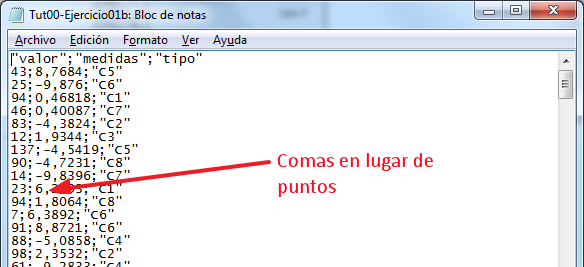
\includegraphics[width=9cm]{../fig/Tut00-EjercicioI-d.png}
        \end{center}
\newcounter{EjercicioII}
\stepcounter{EjercicioII}
\paragraph{Ejercicio \theEjercicioII:}\quad\\
Usando ese mismo fichero,
\begin{enumerate}
  \item Reemplaza el separador de columnas (punto y coma) por el símbolo \verb|#|.
  \item Guarda el fichero modificado con el nombre {\tt Tut00-Ejercicio01c.csv}, y ábrelo en {\em       Calc}. Cuidado con las opciones de importación de ficheros {\tt csv} en Calc, tendrás que
      usar la opción {\tt Otros} para indicar el separador que estamos usando.
  \item Para practicar un poco más el tema de los separadores y la importación de ficheros {\tt
      csv}, aquí tienes el fichero adjunto:
        \begin{center}
            \fichero{../datos/Tut00-Ejercicio01d.csv}{Tut00-Ejercicio01d.csv}
        \end{center}
      que puedes ver en la figura:
        \begin{center}
        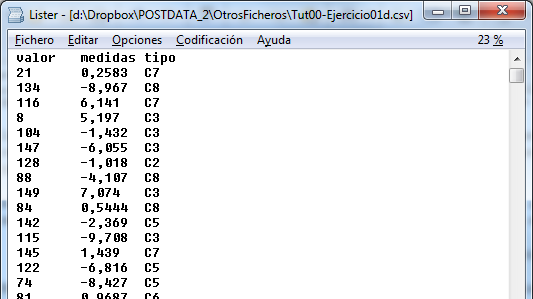
\includegraphics[width=9cm]{../fig/Tut00-EjercicioII.png}
        \end{center}
      Las columnas son más fáciles de reconocer a simple vista porque se han usado {\em
      tabuladores} como separadores entre columnas. Prueba a importar este fichero en Calc.
      Cuando lo hayas hecho, prueba a reemplazar los tabuladores por espacios (ábrelo en el {\em Bloc de Notas} y selecciona un
      tabulador con el ratón, para poder copiarlo y pegarlo en el cuadro de diálogo {\tt
      Reemplazar}). Después, importa ese fichero modificado con Calc. Y, finalmente, cambia los
      separadores por comas, y repite el proceso de importación en Calc. ¿Hay algún problema?
\end{enumerate}
\qed

\section{Instalación de R y RStudio.}

En los tutoriales del curso vamos a utilizar, de forma prioritaria, el programa R. La hoja de
cálculo Calc seguirá acompañándonos, y aprenderemos a hacer con ella muchas otras cosas, pero el
protagonista será R. Por esa razón, vamos a presentar aquí las instrucciones de instalación de R,
en su versión {\tt 3.3.0}. Las instalaciones se refieren a una máquina en la que R {\sf no está
instalado}.
Si ya tienes una versión anterior de R instalado, al final de esta sección encontrarás información sobre la forma de actualizar tu versión de R. \quad\\
La página principal de R (oficialmente R-project), es
\link{http://www.r-project.org/}{www.r-project.org}.
    \begin{center}
    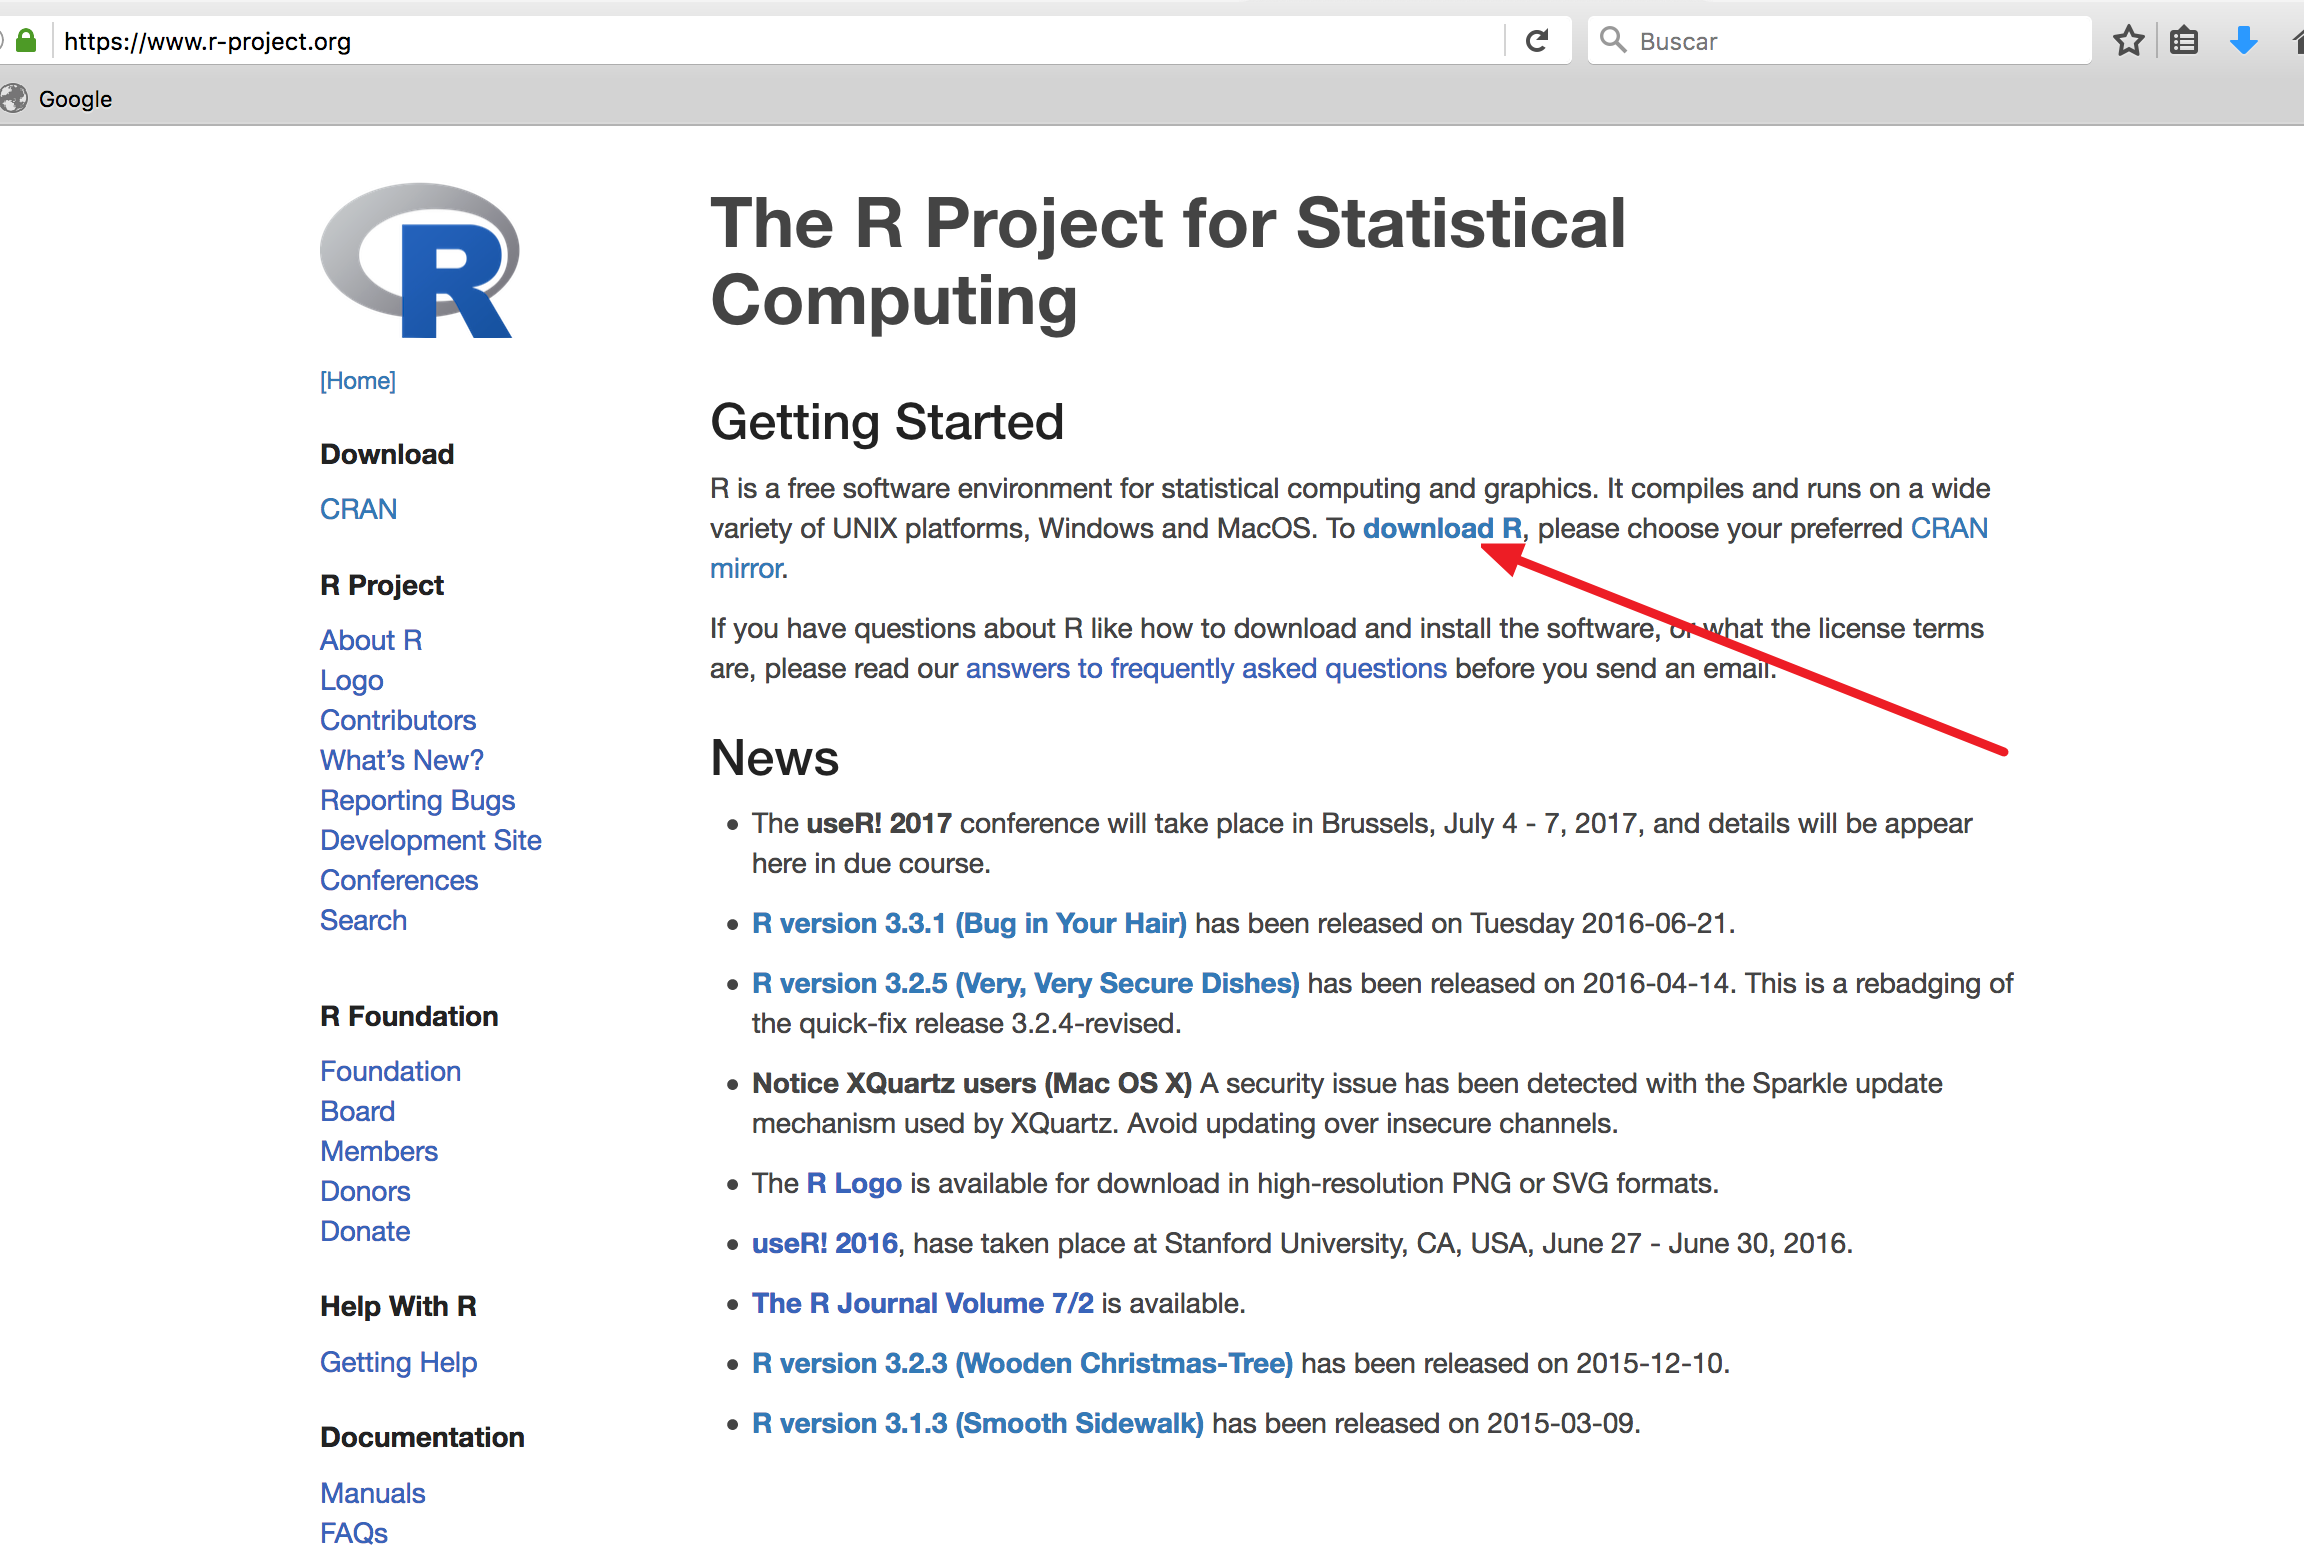
\includegraphics[width=15cm]{../fig/Tut00-35a.png}
    \end{center}
Busca el enlace {\tt download R} (lo he señalado con una flecha roja en la figura, pero puede haber
cambiado de ubicación cuando leas esto). Se abrirá una página en la que debes elegir el repositorio
(mirror) desde el que vas a descargar. En general, conviene elegir uno geográficamente cercano,
para que la conexión sea rápida. El que está situado en España
(\link{https://cran.rediris.es/}{cran.rediris.es}) suele funcionar bien. Al hacer clic sobre el enlace del repositorio llegamos a una página en la que debes decidir según cual sea tu sistema operativo. Aquí veremos las instrucciones para Windows. Haz clic sobre el enlace {\em Download R for Windows} y llegarás a:
    \begin{center}
    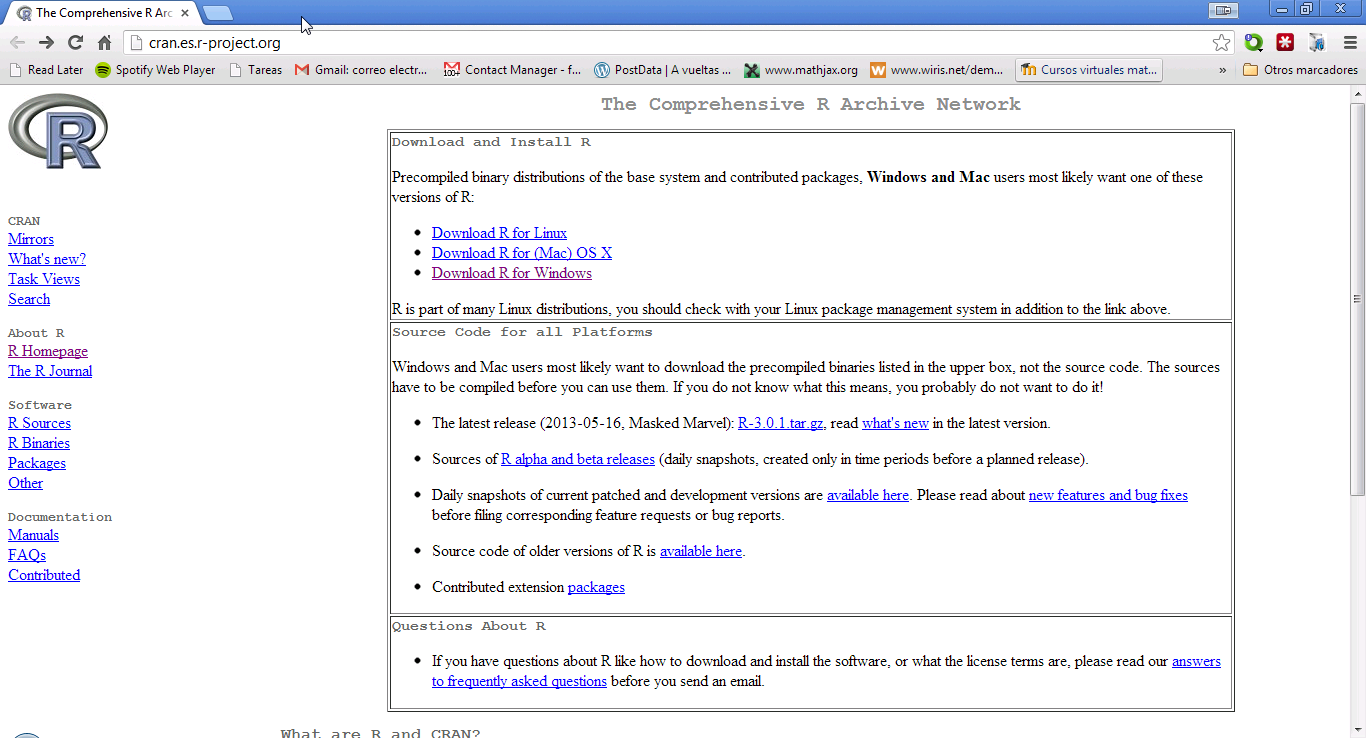
\includegraphics[width=15cm]{../fig/Tut00-36.png}
    \end{center}
 Seguimos el enlace para instalar Windows por primera vez (recuadrado en rojo).
    \begin{center}
    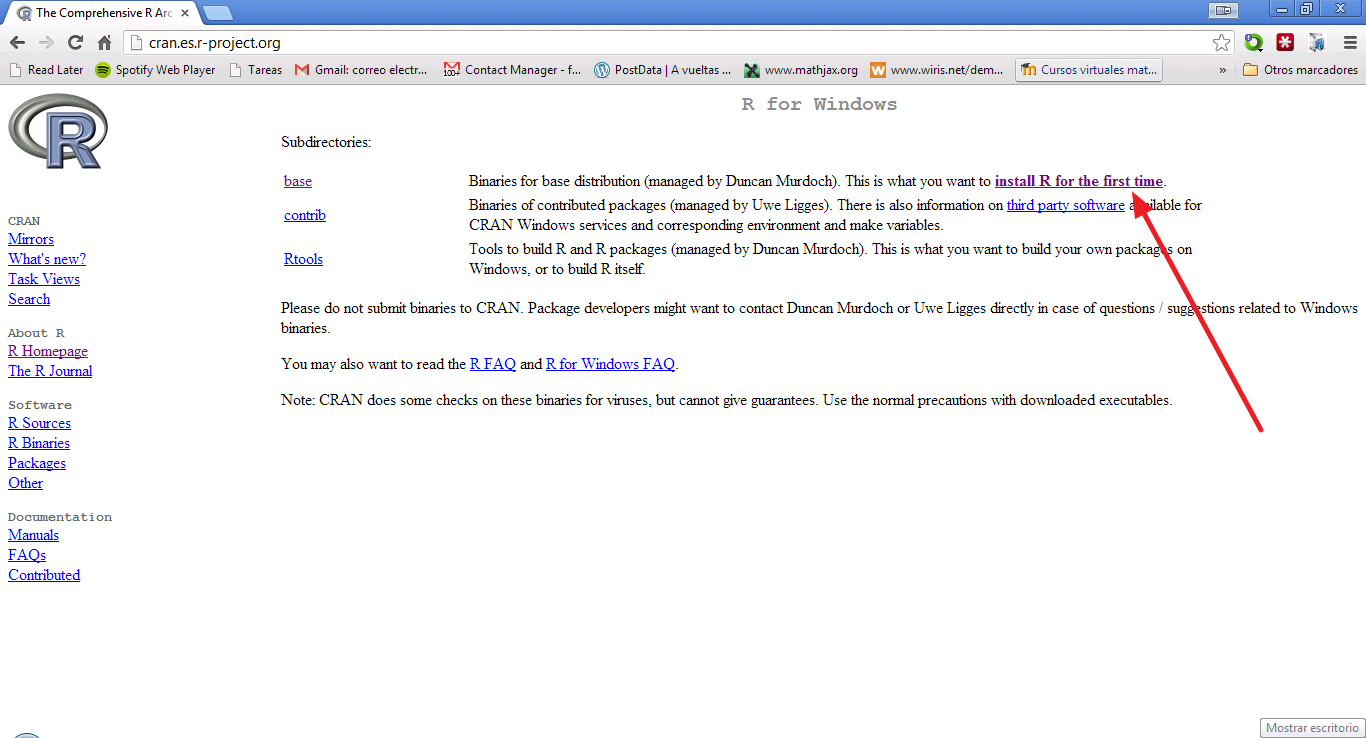
\includegraphics[width=15cm]{../fig/Tut00-37.png}
    \end{center}
Finalmente, llegamos a la página desde la que descargaremos el instalador de la última versión, la
3.3.0 en el momento de escribir esto. El instalador es el
mismo, con independencia de que uses Windows Xp/Windows 7/Windows 8/ Windows 10 (de 32 o 64 bits). 
Descárgalo, y ejecuta el instalador. Puedes aceptar todas las opciones por defecto. La única que te
puede hacer dudar es una en la que se pregunta {\tt ¿Desea utilizar las opciones de
configuración?}. Responde que no, y pulsa en {\tt Siguiente}. Una vez acabada la instalación, en el
{\em Escritorio} o en el menú {\tt Inicio} de Windows, busca un icono como este:
    \begin{center}
    
\includegraphics[width=1cm]{../fig/Tut00-38.png}
    \end{center}
Puedes tener varios de ellos agrupados en un grupo de programas si, por ejemplo, trabajas en Windows de
64 bits. Haz clic en uno cuyo nombre empiece por {\tt R i386} o por {\tt R x64}. En cualquier caso,
si todo va bien, te encontrarás con una ventana muy parecida a esta:
    \begin{center}
    
\includegraphics[width=15cm]{../fig/Tut00-39.png}
    \end{center}
En el futuro, como veremos a continuación, usaremos otra forma, más cómoda, de arrancar R. Usa el menú {\em Archivo} para salir de R (y responde {\em No} a la pregunta sobre guardar la imagen del área de trabajo).

\subsubsection*{Actualizar una versión anterior de R}

Puedes consultar este enlace
\begin{center}
\link{http://fernandosansegundo.wordpress.com/2013/03/22/actualizar-r-en-windows/}{http://fernandosansegundo.wordpress.com/2013/03/22/actualizar-r-en-windows/}
\end{center}

\subsection{Instalación de RStudio.}

Un usuario experto de R puede empezar a trabajar con el programa desde esta misma ventana. Pero
nosotros necesitaremos algo más de ayuda (y los expertos tampoco sufren innecesariamente, si pueden
evitarlo). Así que vamos a instalar otro programa que hará nuestro trabajo con R más sencillo. Ese
programa se llama {\em RStudio}. Antes de instalarlo, cierra la ventana titulada {\tt RGui}. Cuando
lo hagas te preguntará {\tt Save workspace image?} y puedes responder tranquilamente que no.

Para instalar {\em RStudio} nos dirigimos a su página web oficial, en
\link{http://www.rstudio.com/}{www.rstudio.com}.
    \begin{center}
    
\includegraphics[width=9cm]{../fig/Tut00-41a.png}
    \end{center}
y hacemos clic en el enlace que indica la flecha roja. En el siguiente paso elegimos {\tt Download} bajo la columna {\tt RStudio Desktop}
    \begin{center}
    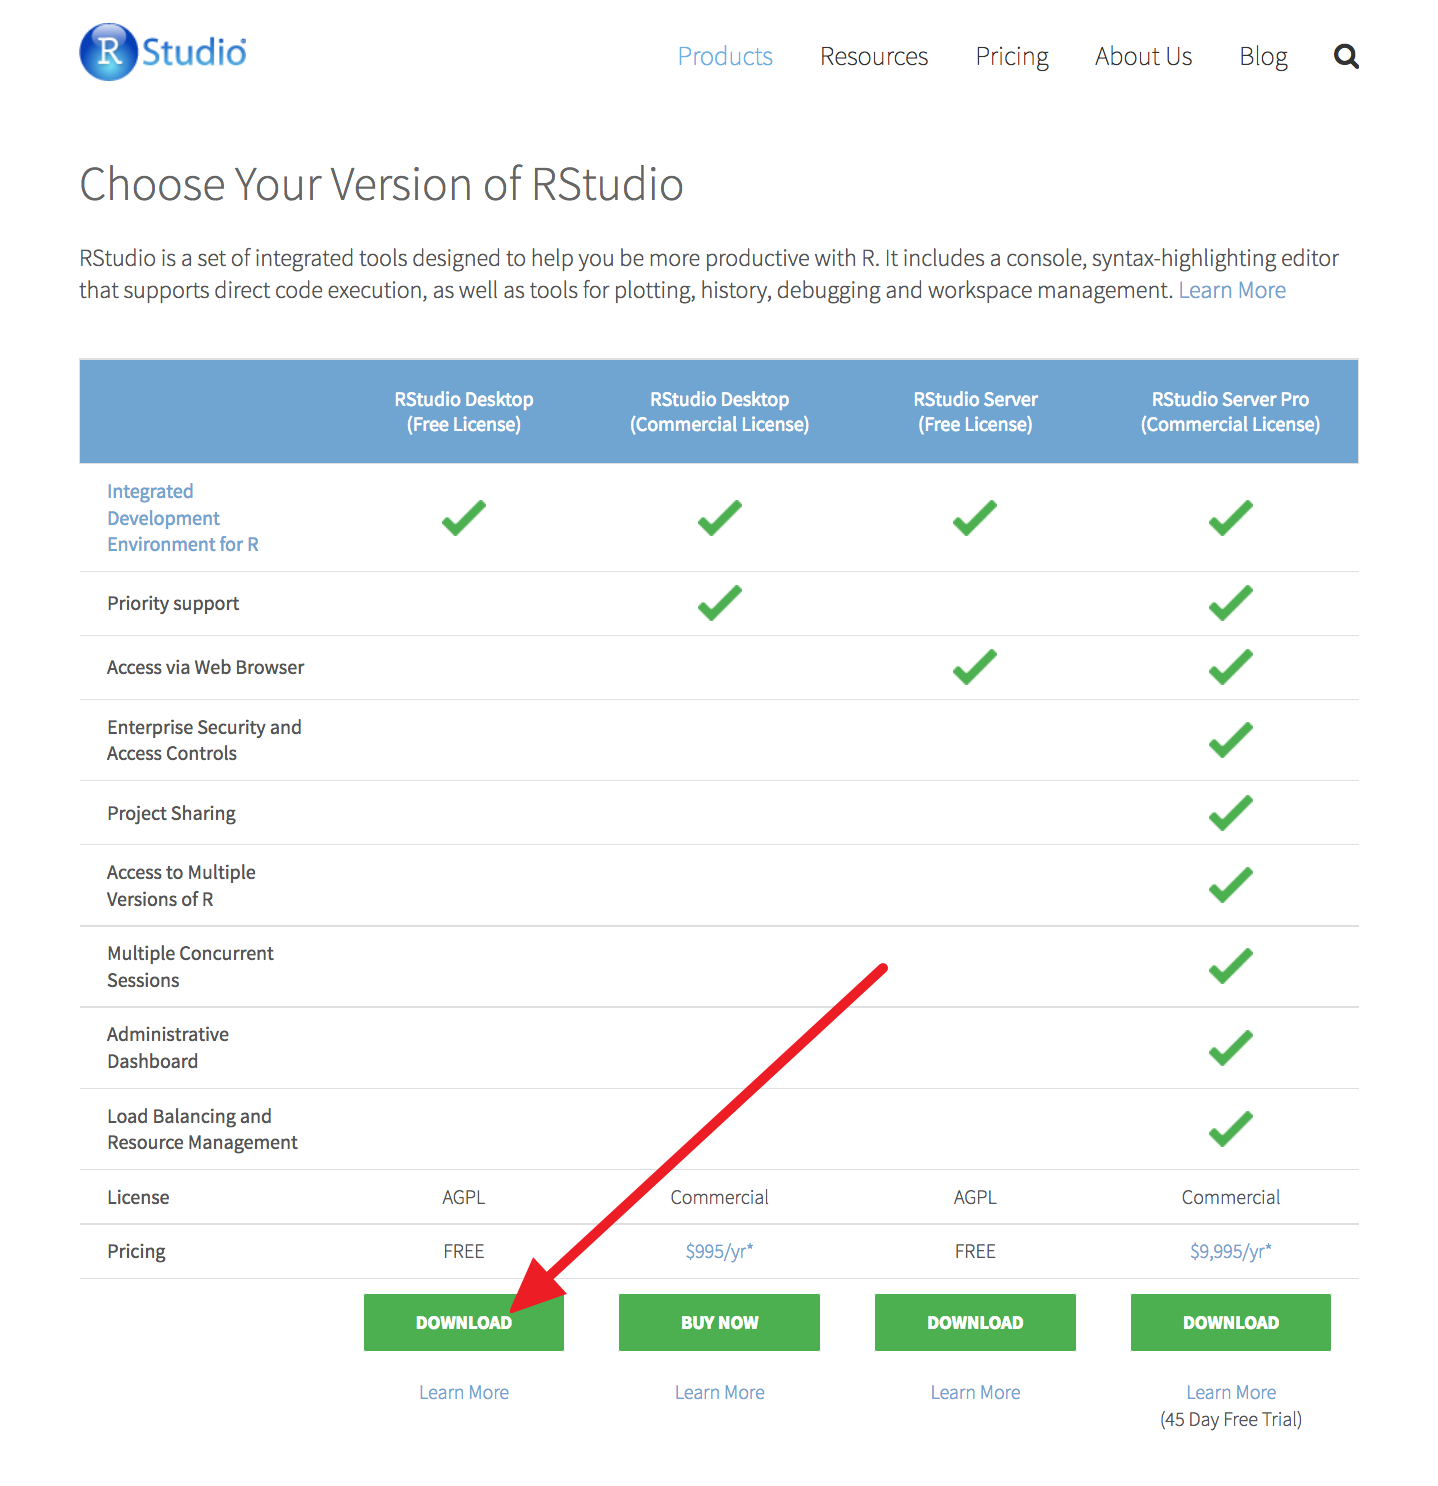
\includegraphics[width=9cm]{../fig/Tut00-42a.png}
    \end{center}
y, finalmente, más abajo en la ventana debemos elegir el instalador adecuado para nuestro 
sistema
%:
%    \begin{center}
%    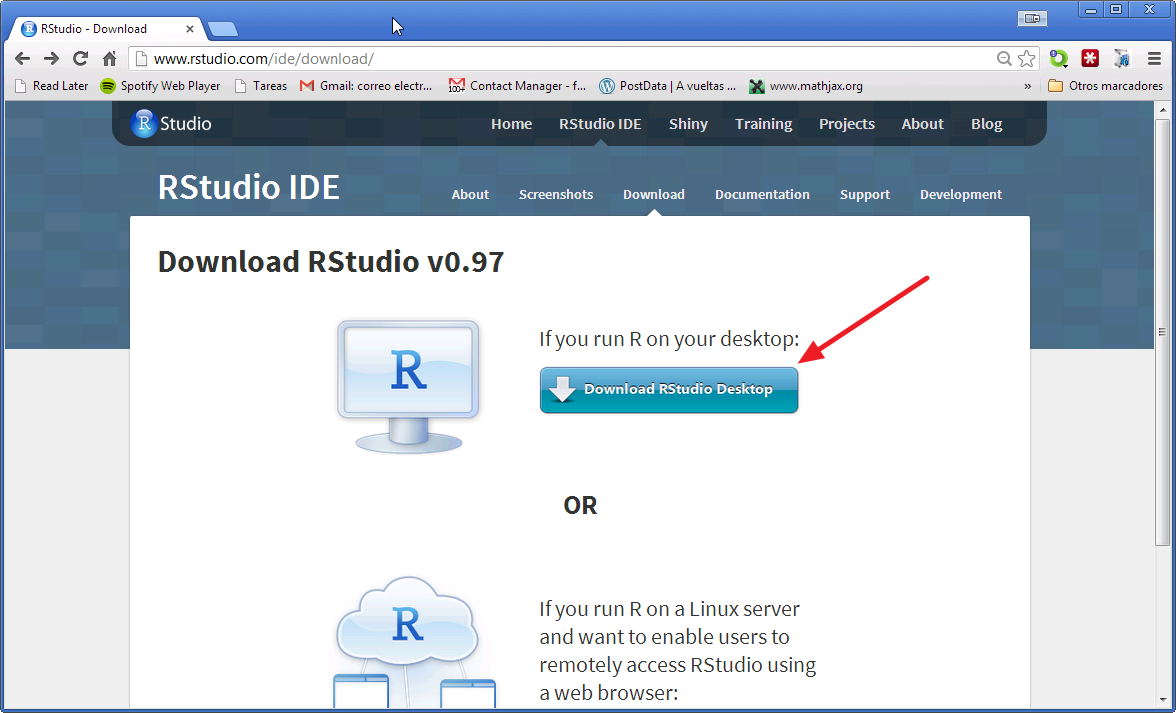
\includegraphics[width=12cm]{../fig/Tut00-42.png}
%    \end{center}
% En mi caso, puesto que he accedido desde una máquina Windows, ese es el sistema que aparece como
% recomendado.
    \begin{center}
    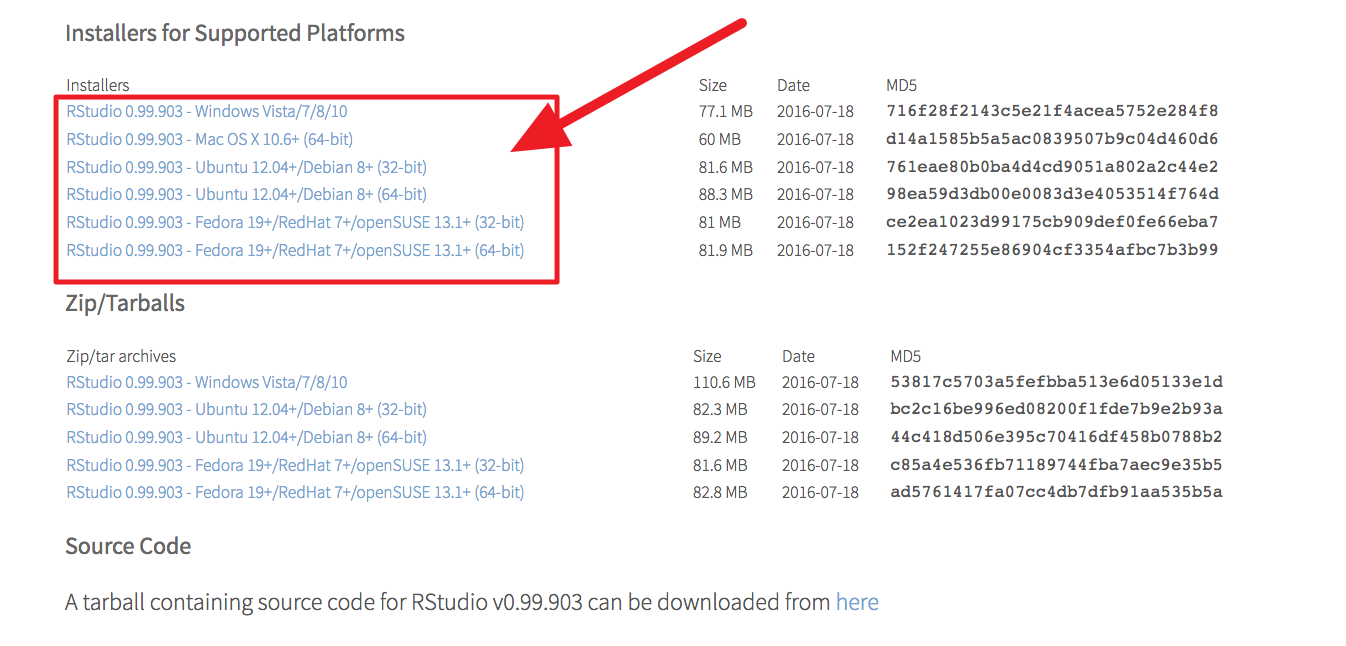
\includegraphics[width=15cm]{../fig/Tut00-43a.png}
    \end{center}
Descarga el instalador que corresponda, y ejecútalo. La instalación no presenta ninguna dificultad,
y una vez terminada, puedes iniciar el programa desde el menu Inicio. El programa, al arrancar,
tiene un aspecto similar a este:
    \begin{center}
    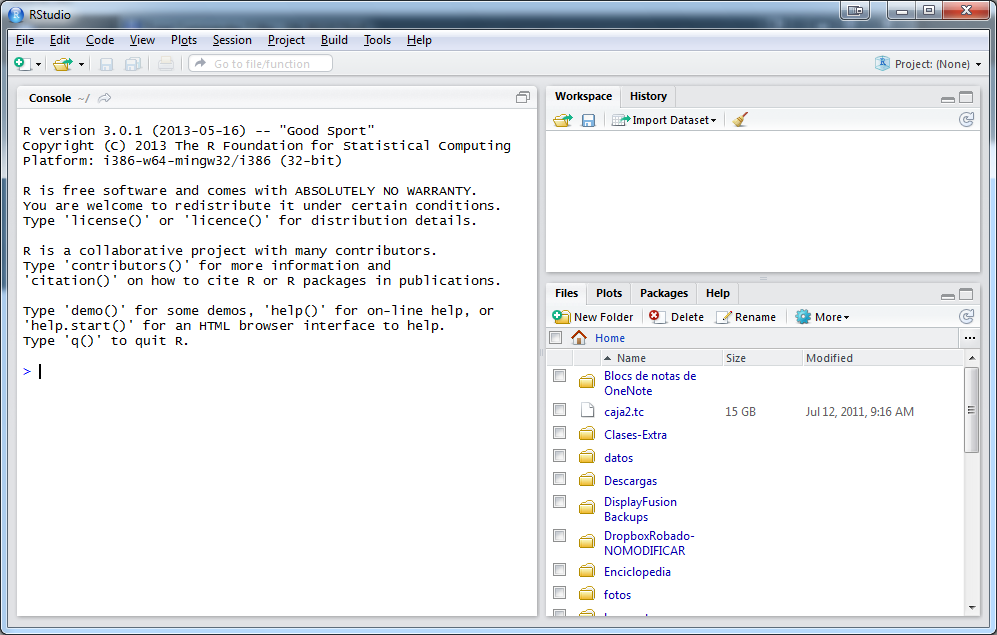
\includegraphics[width=15cm]{../fig/Tut00-44.png}
    \end{center}
Puedes cerrar el programa en este punto. Pronto aprenderemos a usarlo.


\section{Instalación de GeoGebra.}
\label{tut00:sec:InstalacionGeoGebra}

GeoGebra  es un programa gratuito y de código abierto, que, según sus creadores, permite la {\em
interacción dinámica de geometría, álgebra, estadísticas y recursos de análisis y cálculo.}
GeoGebra  se diseñó para servir de apoyo visual a la enseñanza de las matemáticas, y en cada nueva
versión ha ido aumentando sus capacidades. En particular, para lo que aquí nos interesa,  GeoGebra
ofrece bastantes herramientas para trabajar con distribuciones de probabilidad, y algunas
operaciones básicas de la Estadística. En este curso vamos a usar  GeoGebra  sobre todo para
mostrar algunas construcciones dinámicas, en las que podrás interactuar con algunos elementos de la
construcción, para experimentar lo que sucede cuando se modifican.

La página principal del proyecto GeoGebra, en la que puedes encontrar mucha información sobre el
programa es:
\begin{center}
\link{http://www.geogebra.org}{www.geogebra.org}
\end{center}
    \begin{center}
    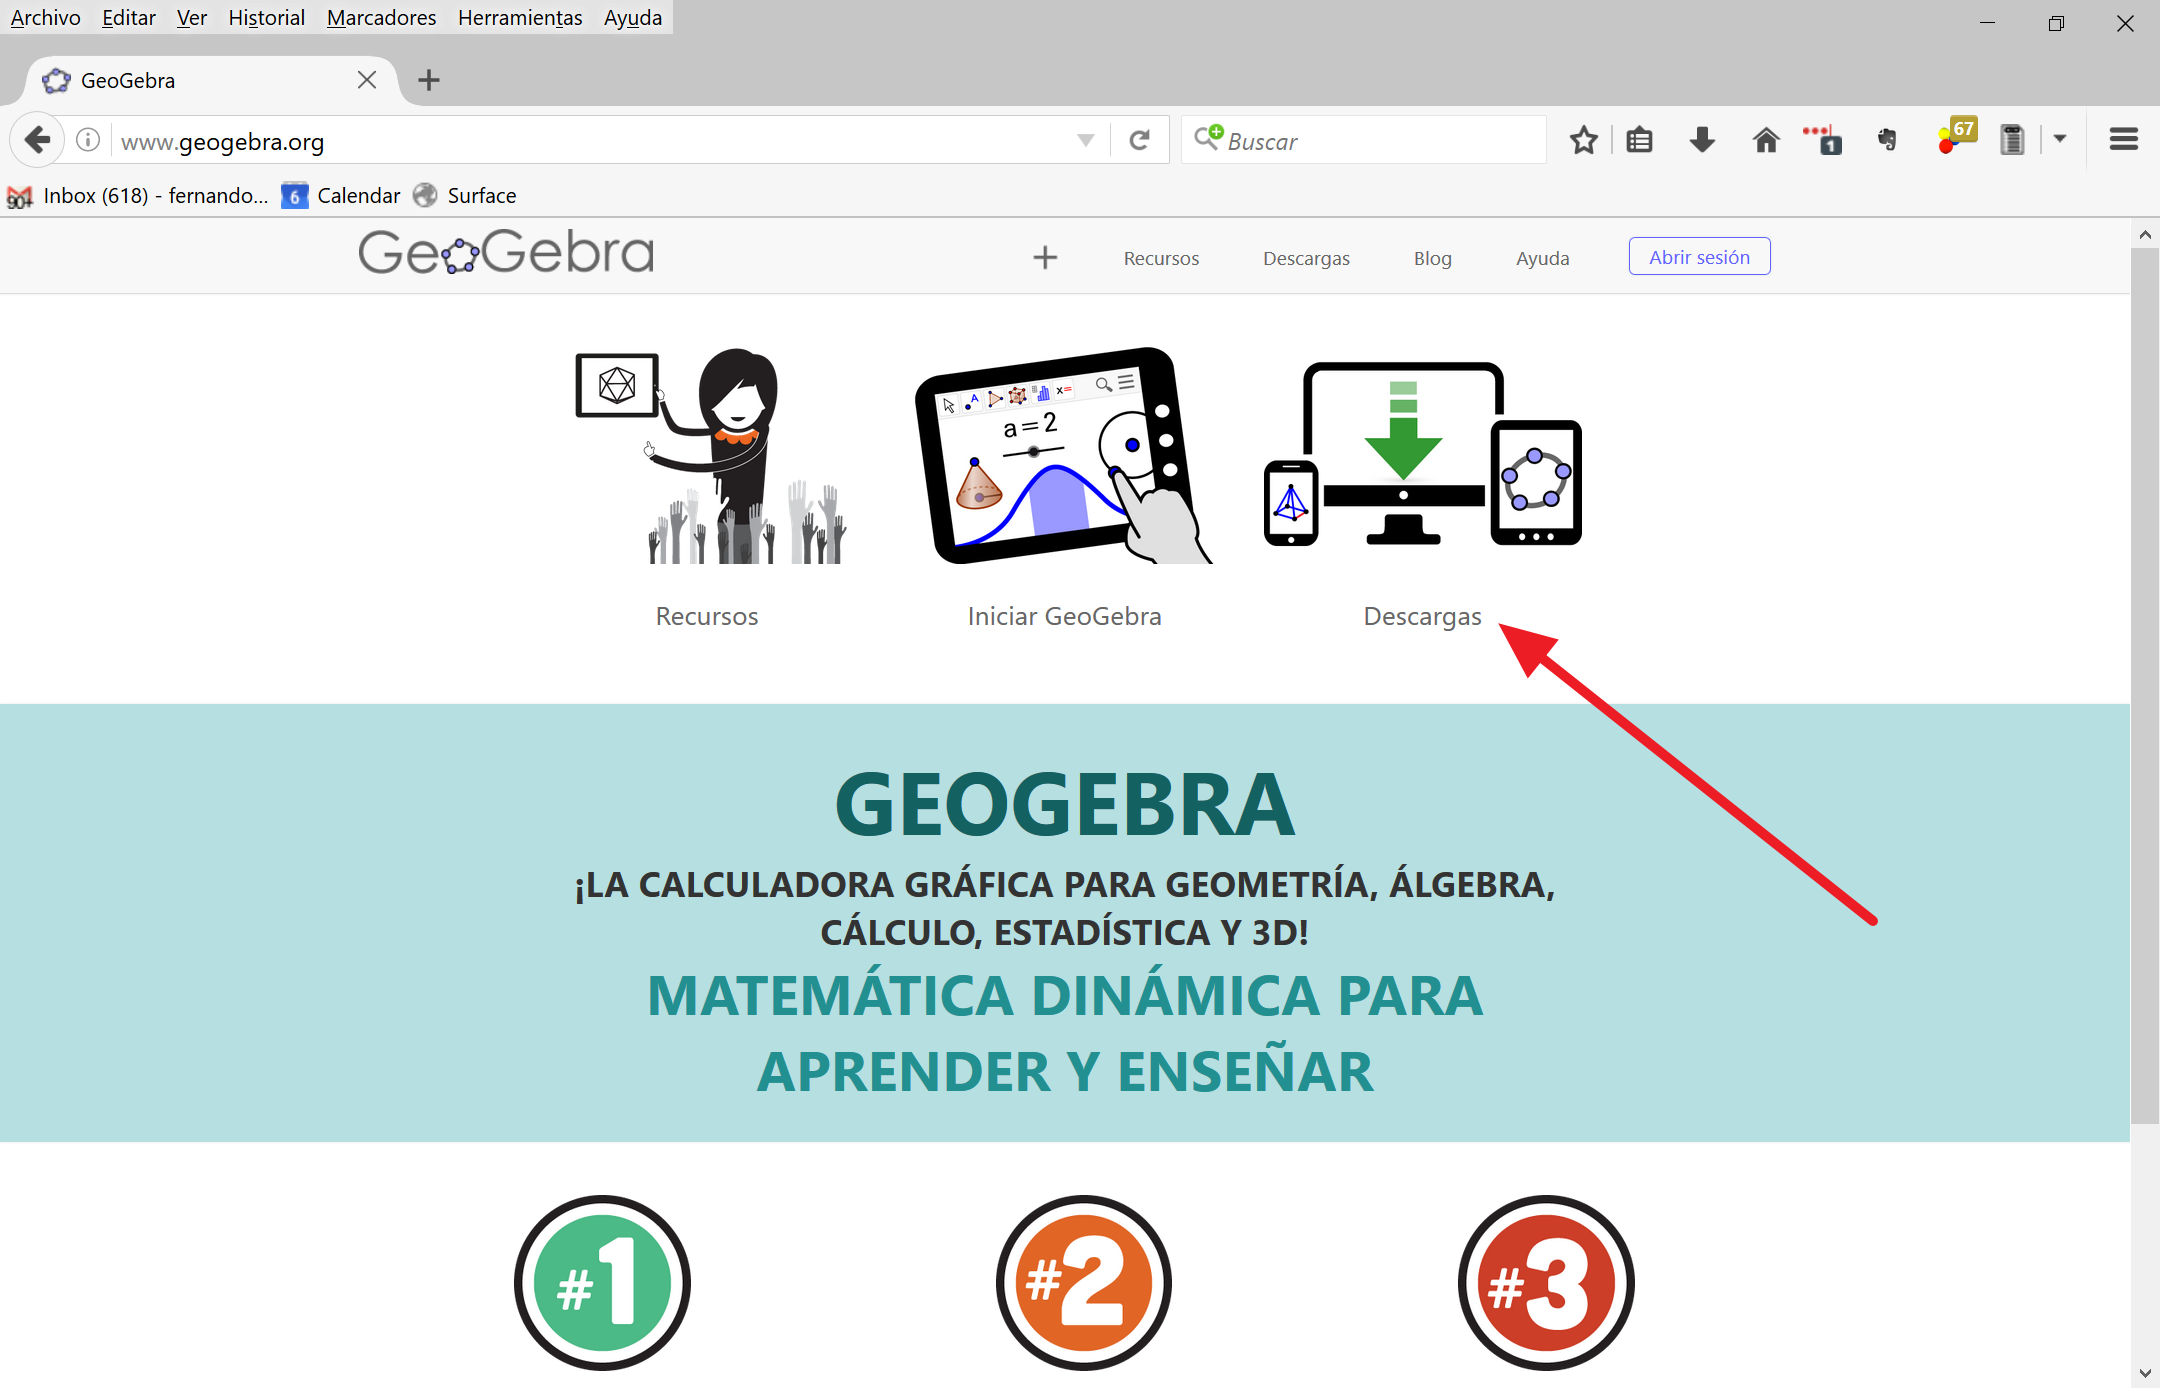
\includegraphics[width=12cm]{../fig/Tut00-GeoGebraDescarga01-201605.png}
    \end{center}
En esa página, pulsa sobre el enlace {\tt Descargas} que hemos destacado en la anterior
figura.
    \begin{center}
    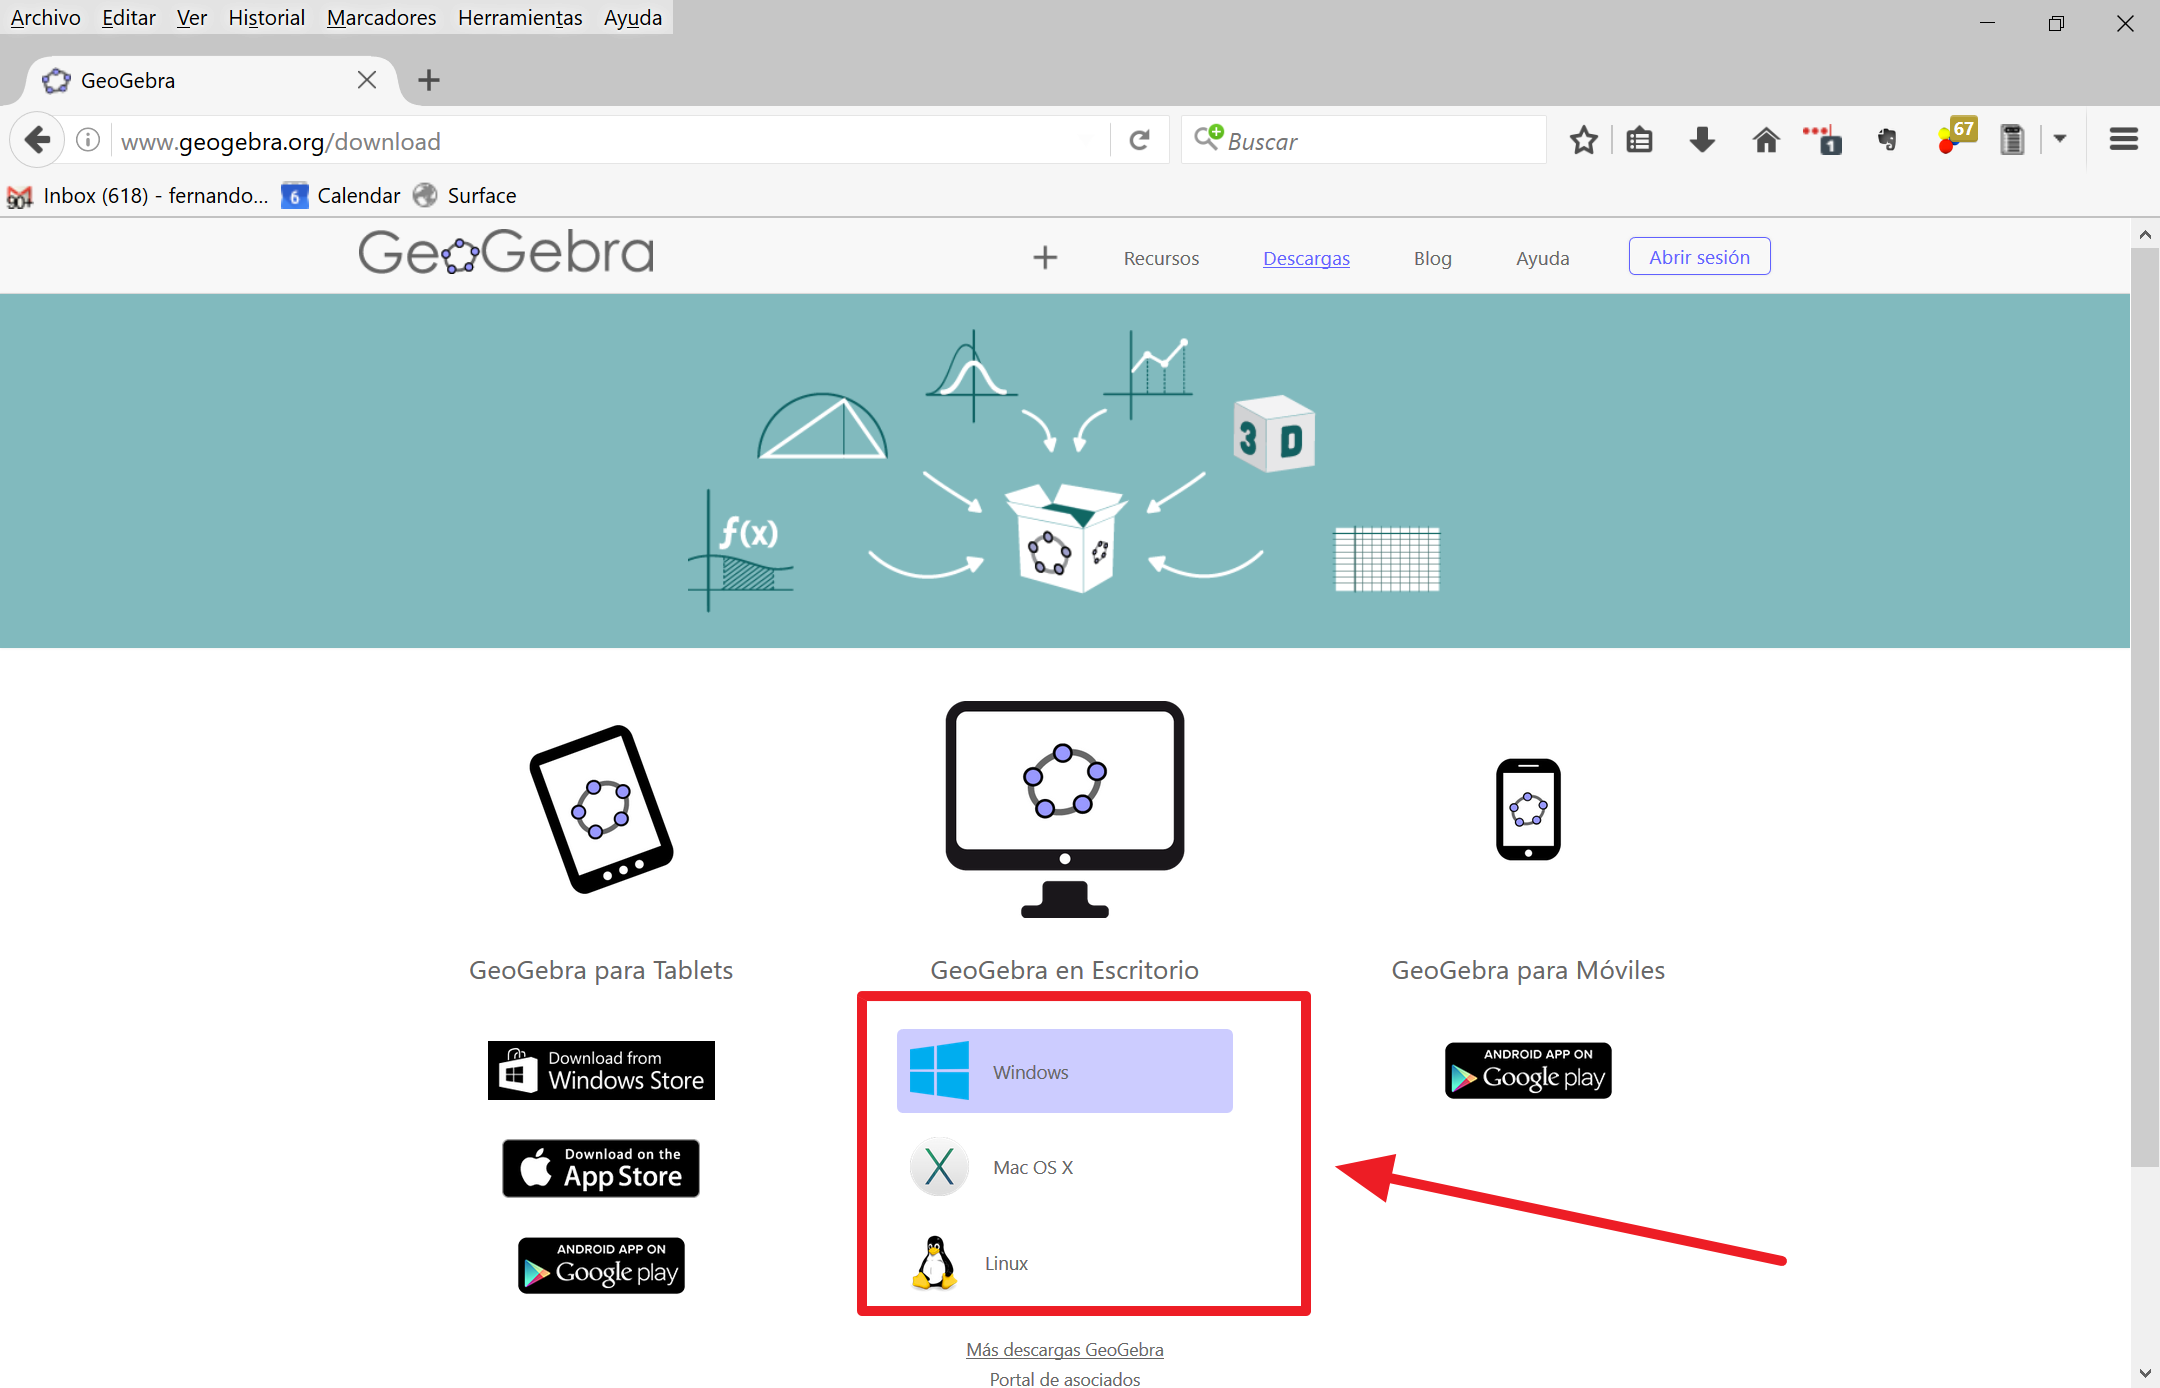
\includegraphics[width=12cm]{../fig/Tut00-GeoGebraDescarga02-201605.png}
    \end{center}
y elige tu sistema en la ventana que se abre. La descarga del instalado debería comenzar en ese
momento. A partir de aquí, las instrucciones de instalación que incluimos son para el sistema
Windows. Tras ejecutar el instalador pasarás por estas pantallas:
    \begin{center}
    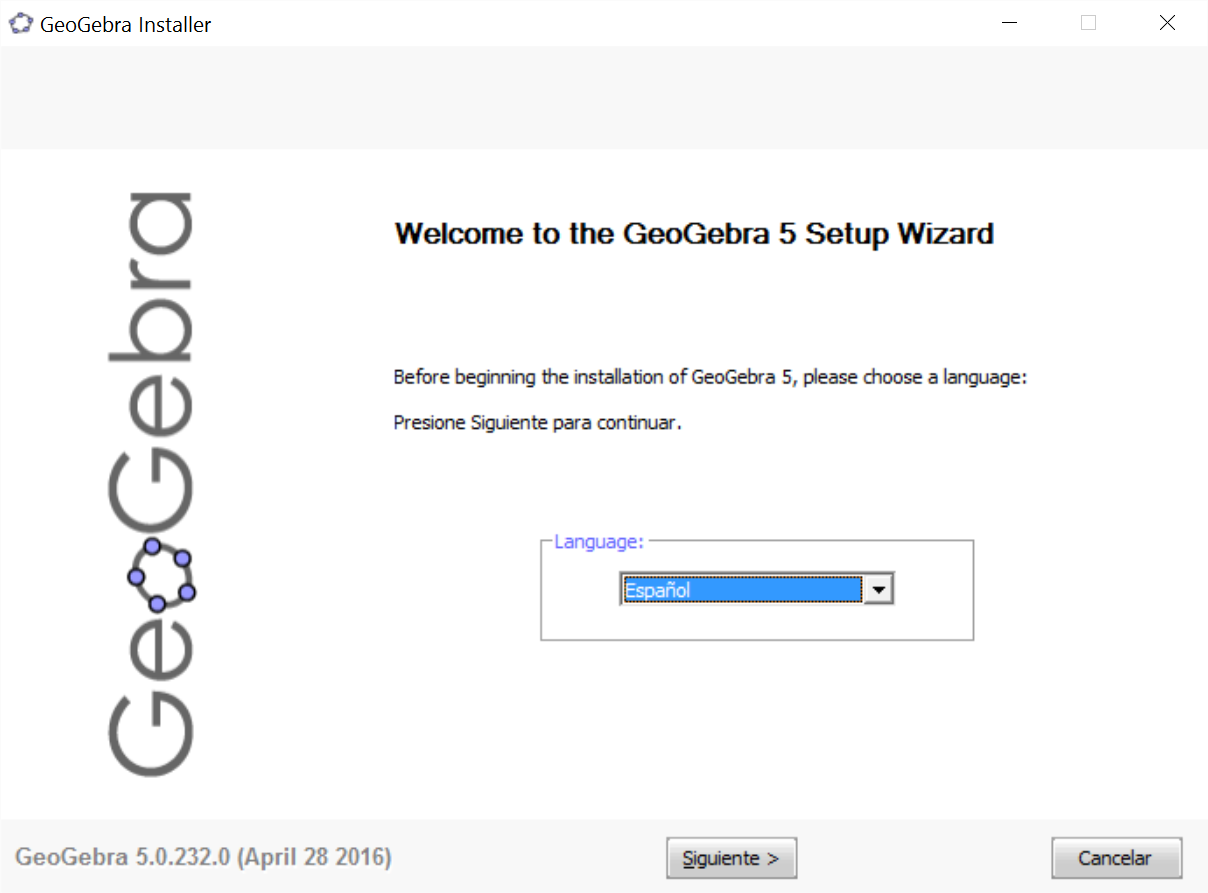
\includegraphics[width=14cm]{../fig/Tut00-GeoGebraSetup01-201605.png}
    \end{center}
Pulsamos en {\tt Siguiente}
    \begin{center}
    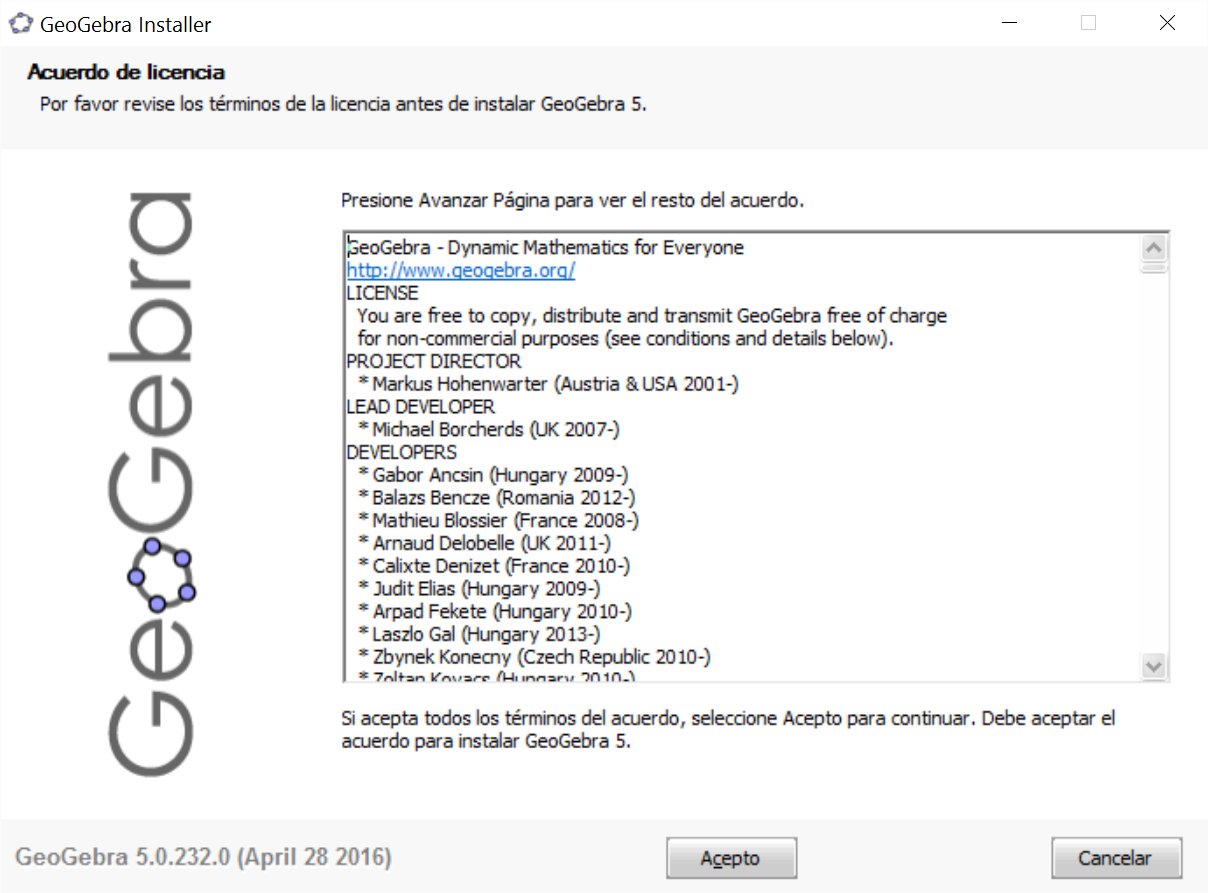
\includegraphics[width=14cm]{../fig/Tut00-GeoGebraSetup02-201605.png}
    \end{center}
Pulsamos en {\tt Acepto}
    \begin{center}
    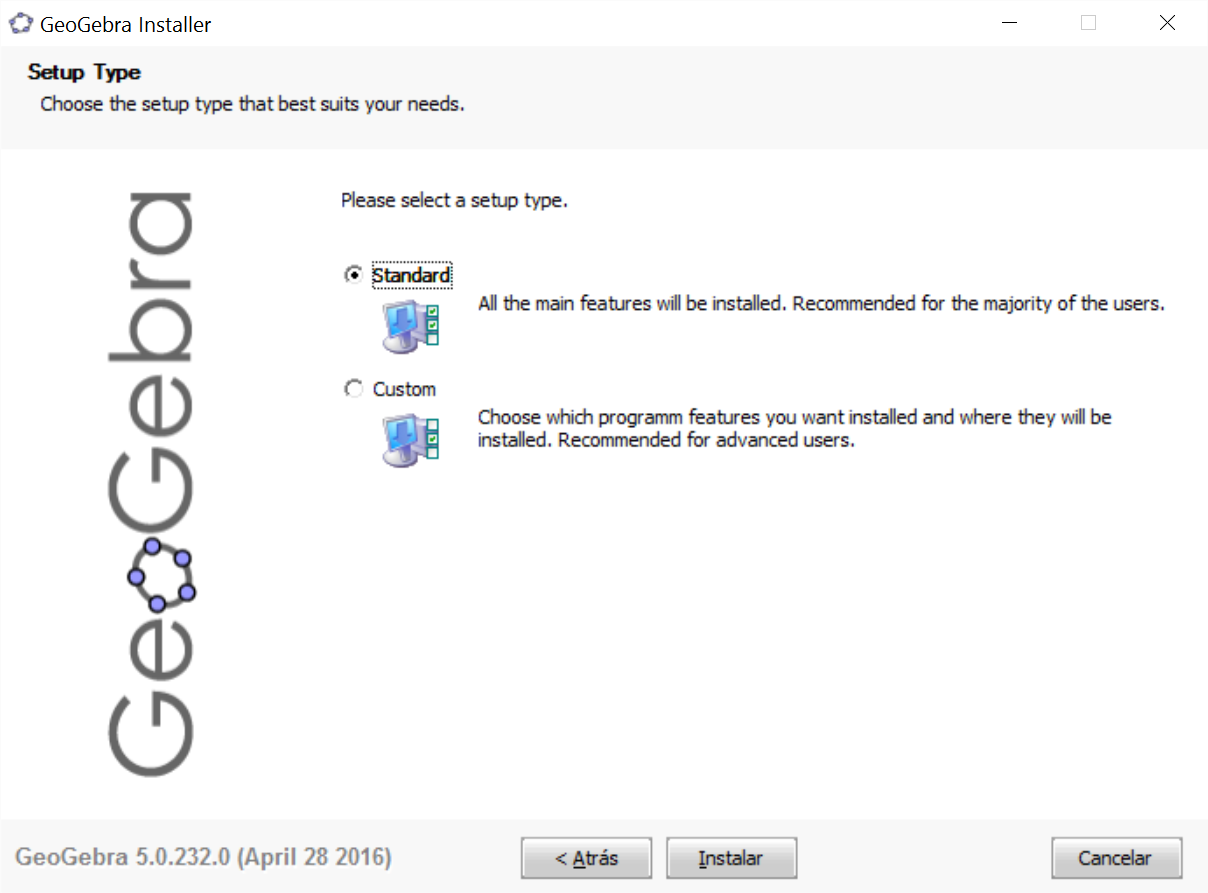
\includegraphics[width=14cm]{../fig/Tut00-GeoGebraSetup03-201605.png}
    \end{center}
Puedes dejar la instalación {\tt Standard} seleccionada, y pulsar en {\tt Instalar}:
    \begin{center}
    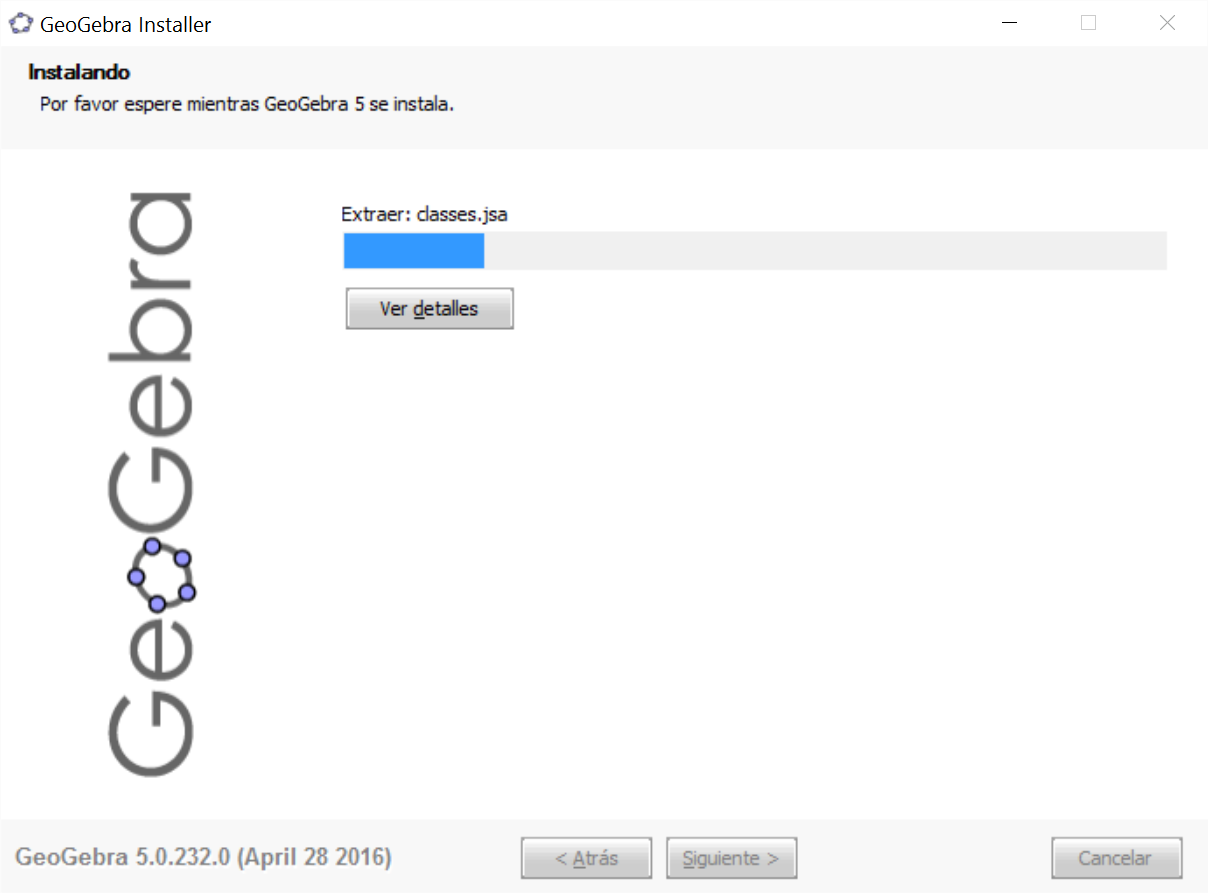
\includegraphics[width=14cm]{../fig/Tut00-GeoGebraSetup04-201605.png}
    \end{center}
Esperamos unos momentos mientras se instala el programa \ldots
    \begin{center}
    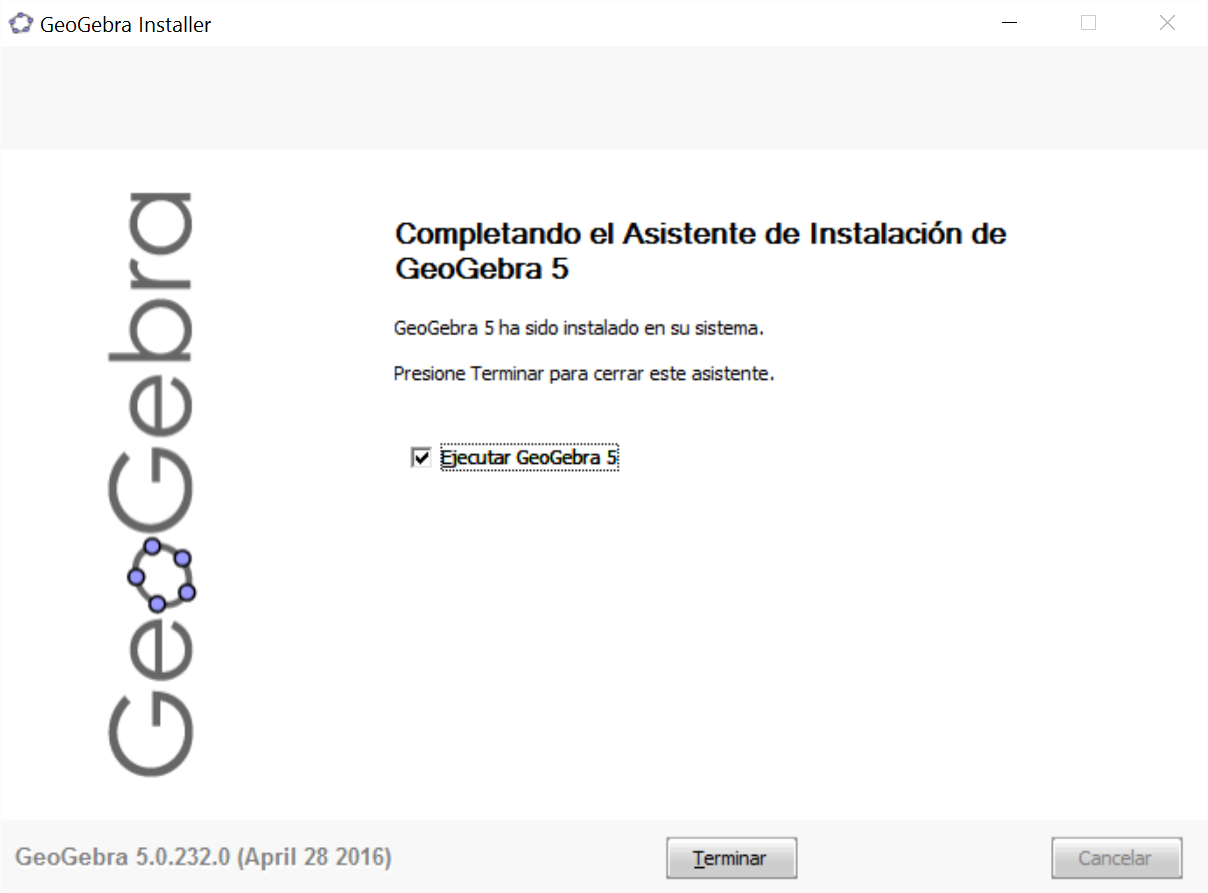
\includegraphics[width=14cm]{../fig/Tut00-GeoGebraSetup05-201605.png}
    \end{center}
\ldots y la instalación concluye correctamente. Para comprobar que ha sido así, deja marcada la
casilla {\tt Ejecutar GeoGebra} y pulsa en {\tt Terminar}. Al cabo de unos instantes aparecerá la
interfaz de GeoGebra, que se muestra en esta figura:
    \begin{center}
    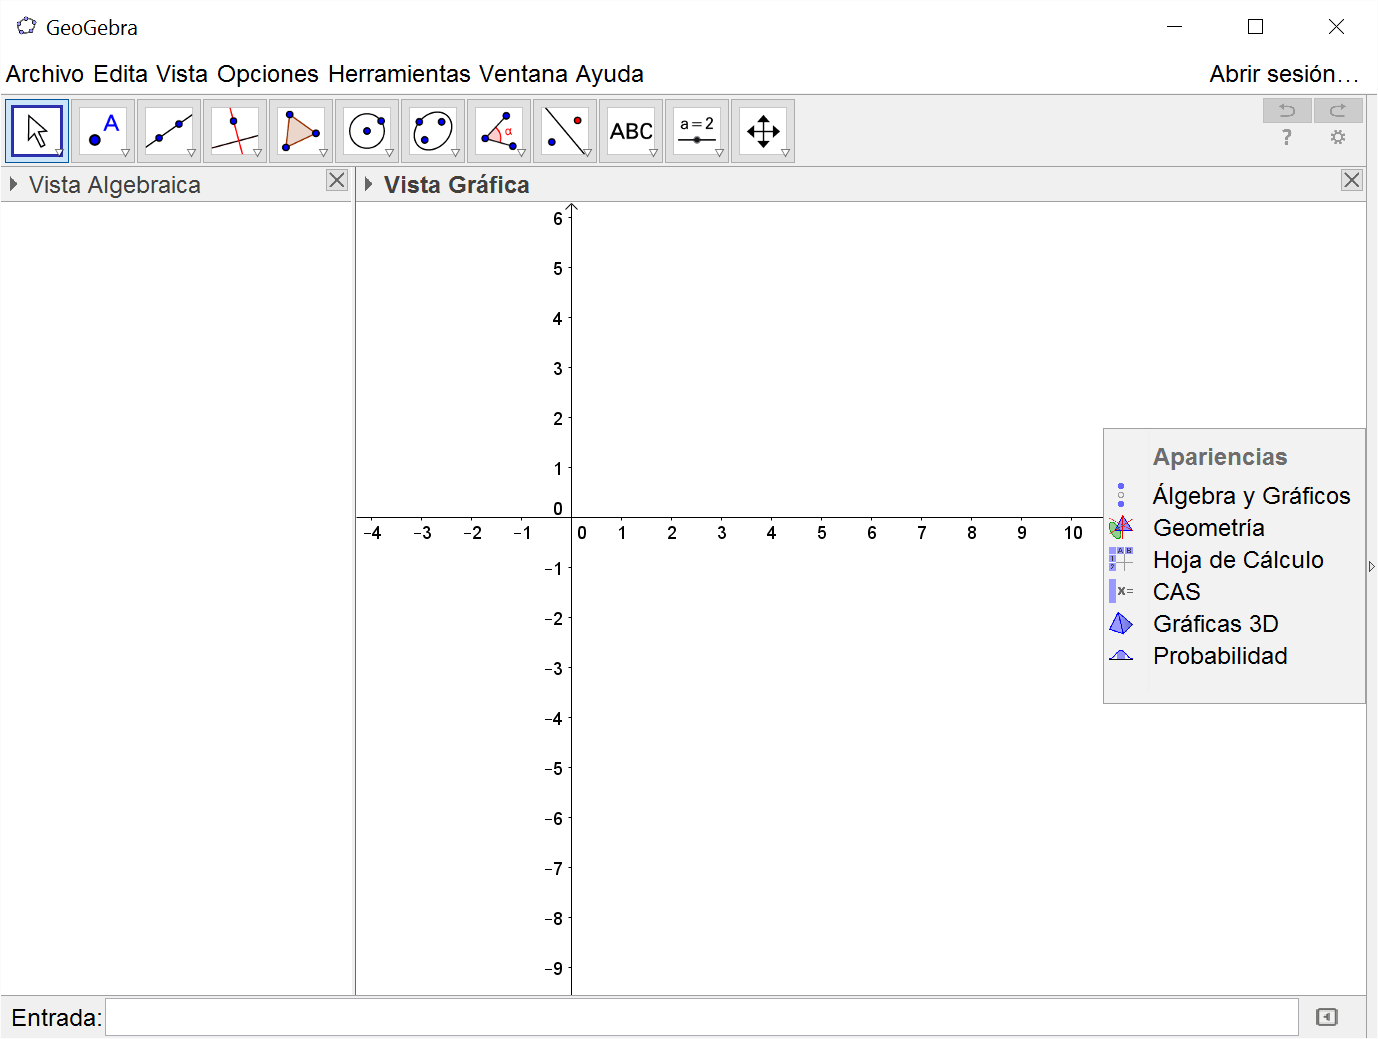
\includegraphics[width=15cm]{../fig/Tut00-GeoGebraSetup06-201605.png}
    \end{center}
Como ves, la mayor parte la ocupa la {\tt Vista Gráfica}, en la que aparecen los ejes de un plano
de coordenadas cartesianas.  Justo debajo aparece la {\em Línea de Entrada}, que usaremos para teclear comandos. En este curso no vamos a profundizar en el uso de GeoGebra. Vamos a usarlo para visualizar construcciones que te entregaremos adjuntas en los capítulos de
teoría o en los tutoriales. Así que podrás usarlas directamente, y ya verás que resultan muy
intuitivas. También usaremos la {\em Calculadora de Probabilidades} y la {\em Ventana de Cálculo Simbólico}, dos herramientas de GeoGebra que facilitarán mucho nuestro trabajo. Pero no vamos a explorar, ni mucho menos, todas las posibilidades que ofrece el programa. En cualquier caso, si quieres aprender más sobre GeoGebra (que es un gran programa para la enseñanza y la visualización de las Matemáticas), te recomendamos que explores su página web.
\section{Siguiente paso. ¿Dónde vamos ahora?}

Tras instalar todo este software, hay que ponerlo a trabajar. En general, como hemos dicho en la Introducción del libro, cada capítulo del libro se corresponde con un tutorial, y la numeración de capítulos y tutoriales coincide. Sin embargo, los Tutoriales 1 y 2, que corresponden a la Parte \ref{curso-parte:EstadisticaDescriptiva} del curso, son especiales. Cada uno de ellos cubre el contenido conjunto de los Capítulos \ref{curso-cap:IntroduccionEstadisticaDescriptiva} y \ref{curso-cap:ValoresCentralesDispersion} de esa parte del curso. Pero en el Tutorial01 se utiliza la hoja de cálculo Calc de OpenOffice, mientras que en el Tutorial02 se usa R.

En el resto del curso, cada pareja Capítulo/Tutorial vendrá acompañada de una {\em Guía de Trabajo}, un documento breve que esencialmente explica como se coordina el trabajo teórico del capítulo con los contenidos prácticos del tutorial. De nuevo, los dos primeros capítulos y tutoriales son un caso especial, porque en este caso existe una única {\em Guía de Trabajo} conjunta para ambos. Y ese es el siguiente paso: debes abrir ese documento y seguir sus instrucciones. El documento estará disponible en la página web del libro, o de la forma que te indique tu profesor. Las {\em Guías de Trabajo} constituirán el guión que ordene nuestro trabajo en el curso.




\vspace{2cm} \hrule
\quad\\
Fin del Tutorial-00. ¡Gracias por la atención!



\end{document}
